% -----------------------------------------------------------------------------------
% This template is brought to you by the Laboratory for                             %
% Electrical Instrumentation and Embedded Systems                                   %
% at the Albert-Ludwigs-Universität in Freiburg                                     %
%                                                                                   %
% Please note: We do not provide technical support for this template                %
% However, please feel free to contribute to this template on GitHub                %
% https://github.com/imtekalex/emes_template                                        %
%                                                                                   %
% Special thanks go out to                                                          %
% Till Steinmann and Andreas Reichenbach                                            %
% -----------------------------------------------------------------------------------

% ToDo:
% Centralize Language settings so that individual chapters are also built correctly.
% Speed up build process

% Document settings

% --------------------------------------------------------------------------------
% Document Class
% --------------------------------------------------------------------------------
% We are using KOMA-Script
\documentclass[
    twoside,  % Default value already set????
    12pt,  % Font size 12pt
    numbers = noendperiod,  % Remove . in the header of a new chapter
    chapterprefix = true,
    bibliography = totoc,  % 
    % listof=totoc, % Adds "List of Figures / Tables" in the ToC
    DIV=calc
] {scrbook}

\usepackage[subpreambles=true]{standalone}
% WARNING: Proceed with caution!

% -----------------------------------------------------------------------------------
% For package standalone
% -----------------------------------------------------------------------------------
\usepackage{import}

% -----------------------------------------------------------------------------------
% Language and typeset
% -----------------------------------------------------------------------------------
\usepackage[ngerman, english]{babel}

% Umlauts and other special characters (UTF-8)
% \usepackage[utf8]{inputenc}
\usepackage{fontspec}
\setsansfont{Arial}
% \usepackage[T1]{fontenc}  % Enable accented characters and umlauts
% LuaLatex doesn't need fontenc and uses UTF-8
% \usepackage{lmodern}  % Font face


% --------------------------------------------------------------------------------
% Page formatting
% --------------------------------------------------------------------------------
% Change the header/footer for chapter beginnings and normal pages
\usepackage[automark,headsepline]{scrlayer-scrpage}

% The package provides an easy and flexible user interface to customize the page
% layout, implementing auto-centering and auto-balancing mechanisms
% WARNING: WHEN CHANGING BCOR (Binding correction), the cover needs reworking!...
\newcommand{\theBCOR}{15mm}  % Define binding correction
\usepackage[
    bindingoffset=\theBCOR,
    % showframe, % Show boxes which indicate margins and paddings
    bottom = 3.5cm, % Margins
      left = 2.5cm,
     right = 2.5cm
] {geometry}

% The package 'float' provides a container for document objects which can not be
% broken over pages, such as tables and figures
% Needed for table and figure indexes  
\usepackage{float}

% support for landscape layout
\usepackage{lscape}

% support of \tablenotes command to add notes under table
\usepackage{threeparttable}

% To allow drawing more professional tables
\usepackage{booktabs}

% --------------------------------------------------------------------------------
% Contents
% --------------------------------------------------------------------------------
% Vector graphics (for Cover page)
\usepackage{tikz} 

% Allows additional parameters when including images
\usepackage{graphicx}

% Roman font family for all headings
\addtokomafont{disposition}{\rmfamily}

% Set the line spacing to 1.5
\usepackage[onehalfspacing]{setspace}

% Improves overall text spacing
% http://www.khirevich.com/latex/microtype/
\usepackage[stretch=10]{microtype}

% Math symbols like mu outside the math environment
\usepackage{textcomp}

% A comprehensive (SI) units package∗
% For defining SI units
\usepackage[
    range-units=single,         % Formatting ranges with single unit indication: 1 - 2 m
    range-phrase=-,             % Phrase for range: 1 - 2 m vs 1 to 2 m
    separate-uncertainty=true,  % sets +- between value and uncertainty 
    multi-part-units=repeat     % In expressions with multiple values (multi part numbers) 
                                % the unit is printed each time: 1 mm x 1 mm
] {siunitx}
% https://tex.stackexchange.com/questions/124488/multi-part-numbers-and-units-in-siunitx

% Allows Sourcecodes with highlighting 
\usepackage{listings}

% This package provides user control over the layout of the three basic list
% environments: enumerate, itemize and description
\usepackage{enumitem}
\setlist{nosep} % Remove the vertical space between \item elements in all lists

% ToDo Notes
% \setlength{\marginparwidth}{2cm}
\usepackage{todonotes}
\setuptodonotes{inline, inlinepar}
\reversemarginpar  % Put ToDo notes on the binding's side
% \usepackage{soul} % Colorful ToDo notes

% Check out colors here http://latexcolor.com/
\usepackage{xcolor}

\usepackage{amsmath}    % alignment of equations

% --------------------------------------------------------------------------------
% Other elements
% --------------------------------------------------------------------------------
% Blindtext: Organic looking text dummy
\usepackage{blindtext}

% Hyperlinks within the document (PDF)
% "hidelinks" hides visual highlighting of links
\usepackage[hidelinks]{hyperref}

% Package for Glossary and Index (Acronyms are listed in a separate list) 
\usepackage[acronym, nogroupskip]{glossaries} % groupskip: alphabetic grouping of entries

\usepackage{xltabular}   % <------- FOR glossaries

% Integration and management of bibliographies
\usepackage{csquotes}   % backend=biber in biblatex needs this package
\usepackage[
    style=ieee,   % style of the bibliography, entries are sorted in alphabetic order. "ieee" is another common style.
    backend=biber,      % based on package 'biber' 
    bibencoding=ascii   % ASCII Text encoding; may use "utf8" instead
] {biblatex}

% --------------------------------------------------------------------------------
%                               PATHS & FILES
% --------------------------------------------------------------------------------
% Fix paths for standalone compiling
\ifstandalone
    \def \home {..}
\else
    \def \home {.}
\fi

% Package: scrlayer-scrpage
% \def \stylePath {\home/settings+/style/page}
% Changing page style for header and footer
\automark{chapter}
\ihead{\leftmark}
\chead{}
\ohead{\thepage}
\ifoot*{}
\cfoot[\thepage]{}
\cfoot*{}
\ofoot*{}
\pagestyle{scrheadings}
  % Load page style

% Package: graphicx
\graphicspath{{\home/images/}}  % Set path to images

% Package: listings
% Change title for list of listings
\renewcommand\lstlistlistingname{\listoflistingstitle{}}

% Code highlighting for C++, you can also add others if needed
\lstset{
    language=C++,
    numbers=left,
    columns=fullflexible,
    aboveskip=5pt,
    belowskip=10pt,
    basicstyle=\small\ttfamily,
    backgroundcolor=\color{black!5},
    commentstyle=\color{darkgreen},
    keywordstyle=\color{blue},
    stringstyle=\color{gray},
    showspaces=false,
    showstringspaces=false,
    showtabs=false,
    xleftmargin=16pt,
    xrightmargin=0pt,
    framesep=5pt,
    framerule=3pt,
    frame=leftline,
    rulecolor=\color{steelblue},
    tabsize=2,
    breaklines=true,
    breakatwhitespace=true,
    prebreak={\mbox{$\hookleftarrow$}}
}
  % Set path to style file
\lstset{inputpath={\home/code/}} % Default path to code listings

% Package: glossaries

% NOT NEEDED? NO CHANGE???
% \glsenablehyper  % activates hyperlink from symbols and acronyms to glossary (symbols and acronyms list)




% Based on entry from Stackexchange
% https://tex.stackexchange.com/questions/269565/glossaries-how-to-customize-list-of-symbols-with-additional-column-for-units
%
% --------------------------------------------------------------------------------
% Style of the Symbols List
% --------------------------------------------------------------------------------
% Title of Symbols List
\newglossary[slg]{symbolslist}{syi}{syg}{\symbolslisttitle{}}

% Use addkey because we want three columns
% It's a mystery, but works 
\glsaddkey{unit}                    % new key
    {\glsentrytext{\glslabel}}      % entry text with default value
    {\glsentryunit}                 % commands which seem only to differ in the 
                                    % number of upper case letters
    {\GLsentryunit}
    {\glsunit}                      % command analogous to \glstext (function for 
                                    % link text (text produced by \gls{}), 
                                    % all lower case) 
    {\Glsunit}                      % command analogous to \Glstext (function for 
                                    % link text (text produced by \gls{}), 
                                    % first letter upper case)
    {\GLSunit}                      % command analogous to \GLStext (function for 
                                    % link text (text produced by \gls{}), all 
                                    % upper case)

\makeglossaries  % activate glossaries-package

\newglossarystyle{symbstyle} {
    \setglossarystyle{long3col}  % base this style on the list style
    \renewenvironment{theglossary} {
        % Change the table type --> 3 columns
        \xltabular{\linewidth}{p{0.2\textwidth}Xp{0.1\textwidth}}
    }{
        \endxltabular
    }

    %  Change the table header / footer
    \renewcommand*{\glossaryheader} {
        \bfseries \symbolslistname & \bfseries \symbolslistdescription & \bfseries \symbolslistunit \\
        \hline \endfirsthead
        \hline \endfoot
    }

    % Change the displayed items
    \renewcommand*{\glossentry}[2] {
        \glstarget{##1}{\glossentryname{##1}} & \glossentrydesc{##1} & \glsunit{##1} \\
        %               Symbol                      Description            Unit
    }
}  % Set path to symbols list style file
% Based on entry from Stackexchange
% https://tex.stackexchange.com/questions/269565/glossaries-how-to-customize-list-of-symbols-with-additional-column-for-units
%
% --------------------------------------------------------------------------------
% Style of the Acronyms List
% --------------------------------------------------------------------------------
\newglossarystyle{acrostyle} {
    %\setglossarystyle{long3col}   % base this style on the list style
    \renewenvironment{theglossary} {  % Change the table type --> 2 columns
        \xltabular{\linewidth}{p{0.2\textwidth}X}
    }{
        \endxltabular
    }

    % Change the table header
    \renewcommand*{\glossaryheader} {
        \bfseries \acronymstitle{} & \bfseries \acronymsdescription{} \\
        \hline
        \endfirsthead
        \hline\endfoot
    }

    % \renewcommand*{\glsgroupheading}[1]{}

    \renewcommand*{\glossaryentryfield}[5]{
        \glstarget{##1}{##2} & \glsentrydesc{##1}\\
    }

    % \renewcommand*{\glossarysubentryfield}[6]{ 
    %     &
    %     \glssubentryitem{##2} 
    %     \glstarget{##2}{\strut}##4 & ##6\\
    % }
 
    %*** GROUP SKIP *** 
    %\renewcommand*{\glsgroupskip}{&\\}% 
    %\renewcommand*{\glsgroupskip}{\addlinespace}% 
    %******************
}
  % Set path to acronym list style file
% -------------------------------------------------------------------------------
%               Listing of all Glossary and Acronym Entries 
%                           use as shown below
% -------------------------------------------------------------------------------

% ==== EXEMPLARY ENTRY FOR SYMBOLS LIST =========================================
\newglossaryentry{symb:Pi} {
    name=$\pi$,
    description=Geometrical value,
    unit=-,
    type=symbolslist
}

\newglossaryentry{symb:height} {
    name={$h$},
    description={Height},
    unit={\si{m}},
    type=symbolslist
}

\newglossaryentry{symb:energy} {
    name={$P$},
    description={Energy consumption},
    unit={\si{kW}},
    type={symbolslist}
}

\newglossaryentry{symb:A} {
    name=A,
    description=Geometrical value,
    unit=-,
    type=symbolslist
}

\newglossaryentry{symb:B} {
    name=B,
    description={Height},
    unit={\si{m}},
    type=symbolslist
}

\newglossaryentry{symb:C} {
    name=C,
    description={Energy consumption},
    unit={\si{kW}},
    type={symbolslist}
}

\newglossaryentry{symb:D} {
    name=D,
    description=Geometrical value,
    unit=-,
    type=symbolslist
}

\newglossaryentry{symb:E} {
    name=E,
    description={Height},
    unit={\si{m}},
    type=symbolslist
}

\newglossaryentry{symb:F} {
    name=F,
    description={Energy consumption},
    unit={\si{kW}},
    type={symbolslist}
}


\newglossaryentry{symb:G} {
    name=G,
    description=Geometrical value,
    unit=-,
    type=symbolslist
}

\newglossaryentry{symb:H} {
    name=H,
    description={Height},
    unit={\si{m}},
    type=symbolslist
}

\newglossaryentry{symb:I} {
    name=I,
    description={Energy consumption},
    unit={\si{kW}},
    type={symbolslist}
}

\newglossaryentry{symb:J} {
    name=J,
    description=Geometrical value,
    unit=-,
    type=symbolslist
}

\newglossaryentry{symb:K} {
    name=K,
    description={Height},
    unit={\si{m}},
    type=symbolslist
}

\newglossaryentry{symb:L} {
    name=L,
    description={Energy consumption},
    unit={\si{kW}},
    type={symbolslist}
}
\newglossaryentry{symb:M} {
    name=A,
    description=Geometrical value,
    unit=-,
    type=symbolslist
}

\newglossaryentry{symb:N} {
    name=B,
    description={Height},
    unit={\si{m}},
    type=symbolslist
}

\newglossaryentry{symb:O} {
    name=C,
    description={Energy consumption},
    unit={\si{kW}},
    type={symbolslist}
}

\newglossaryentry{symb:P} {
    name=D,
    description=Geometrical value,
    unit=-,
    type=symbolslist
}

\newglossaryentry{symb:Q} {
    name=E,
    description={Height},
    unit={\si{m}},
    type=symbolslist
}

\newglossaryentry{symb:R} {
    name=F,
    description={Energy consumption},
    unit={\si{kW}},
    type={symbolslist}
}


\newglossaryentry{symb:S} {
    name=G,
    description=Geometrical value,
    unit=-,
    type=symbolslist
}

\newglossaryentry{symb:T} {
    name=H,
    description={Height},
    unit={\si{m}},
    type=symbolslist
}

\newglossaryentry{symb:U} {
    name=I,
    description={Energy consumption},
    unit={\si{kW}},
    type={symbolslist}
}

\newglossaryentry{symb:V} {
    name=J,
    description=Geometrical value,
    unit=-,
    type=symbolslist
}

\newglossaryentry{symb:W} {
    name=K,
    description={Height},
    unit={\si{m}},
    type=symbolslist
}

\newglossaryentry{symb:X} {
    name=L,
    description={Energy consumption},
    unit={\si{kW}},
    type={symbolslist}
}

\newglossaryentry{symb:Y} {
    name=L,
    description={Energy consumption},
    unit={\si{kW}},
    type={symbolslist}
}

\newglossaryentry{symb:Z} {
    name=L,
    description={Energy consumption},
    unit={\si{kW}},
    type={symbolslist}
}

% ==== EXEMPLARY ENTRY FOR ACRONYMS LIST ========================================
% \newacronym{#label}{#acronym}{#long_form}

% define new command for custom arconym entry with only two arguments
% fabricates an easier way to use \newacronym 
\newcommand{\acroX}[2]{\newacronym{#1}{#1}{#2}}
% \acroX{label and arconym}{long name}
% \acroX{CD}               {Compact Disk}

\newcommand{\acroY}[3]{\newacronym{#1}{#2}{#3}}
% \arcoY{label}{acronym}{long name}
% \acroY{CD}   {cd}     {Compact Disk}
 
\newacronym{VRBD}  {VRBD}   {Violet-Red-Bile-Glucose-Agar}
\newacronym{lan}   {LAN}    {Local Area Network}
\newacronym{din}   {DIN}    {Deutsches Institut für Normung}
\newacronym{iso}   {ISO}    {Internationale Organisation für Normung}
\newacronym{sas}   {SAS}    {Serial Attached SCSI}
\newacronym{abbvz} {Abbvz.} {Abbildungsverzeichnis}
\newacronym{aA}    {VRBD}   {Violet-Red-Bile-Glucose-Agar}
\newacronym{aB}    {CD}     {Compact Disk}
\newacronym{aC}    {LAN}    {Local Area Network}
\newacronym{aD}    {DIN}    {Deutsches Institut für Normung}
\newacronym{aE}    {ISO}    {Internationale Organisation für Normung}
\newacronym{aF}    {SAS}    {Serial Attached SCSI}
\newacronym{aG}    {Abbvz.} {Abbildungsverzeichnis}
\newacronym{aH}    {VRBD}   {Violet-Red-Bile-Glucose-Agar}
\newacronym{aI}    {CD}     {Compact Disk}
\newacronym{aJ}    {LAN}    {Local Area Network}
\newacronym{aK}    {DIN}    {Deutsches Institut für Normung}
\newacronym{aL}    {ISO}    {Internationale Organisation für Normung}
\newacronym{aM}    {SAS}    {Serial Attached SCSI}
\newacronym{aN}    {Abbvz.} {Abbildungsverzeichnis}
\newacronym{aO}    {VRBD}   {Violet-Red-Bile-Glucose-Agar}
\newacronym{aP}    {CD}     {Compact Disk}
\newacronym{aQ}    {LAN}    {Local Area Network}
\newacronym{aR}    {DIN}    {Deutsches Institut für Normung}
\newacronym{aS}    {ISO}    {Internationale Organisation für Normung}
\newacronym{aT}    {SAS}    {Serial Attached SCSI}
\newacronym{aU}    {Abbvz.} {Abbildungsverzeichnis}
\newacronym{aV}    {CD}     {Compact Disk}
\newacronym{aW}    {LAN}    {Local Area Network}
\newacronym{aX}    {DIN}    {Deutsches Institut für Normung}
\newacronym{aY}    {ISO}    {Internationale Organisation für Normung}
\newacronym{aZ}    {SAS}    {Serial Attached SCSI}


% ==== EXEMPLARY ENTRY FOR MAIN GLOSSARY ========================================
    \newglossaryentry{Biofouling} {
        name=Biofouling,
        description={Some description}}
    
    \newglossaryentry{berlin} {
        name={Berlin},
        description={Berlin ist die Bundeshauptstadt der Bundesrepublik Deutschland und zugleich eines ihrer Länder. Die Stadt Berlin ist mit über 3,4 Millionen Einwohnern die bevölkerungsreichste und mit 892 Quadratkilometern die flächengrößte Gemeinde Deutschlands sowie nach Einwohnern die zweitgrößte der Europäischen Union. Sie bildet das Zentrum der Metropolregion Berlin/Brandenburg (6 Millionen Einw.) und der Agglomeration Berlin (4,4 Millionen Einw.). Der Stadtstaat unterteilt sich in zwölf Bezirke. Neben den Flüssen Spree und Havel befinden sich im Stadtgebiet kleinere Fließgewässer sowie zahlreiche Seen und Wälder}
        }
    \newglossaryentry{outsourcing} {
        name={Outsourcing},
        description={Outsourcing bzw. Auslagerung bezeichnet in der Ökonomie die Abgabe von Unternehmensaufgaben und -strukturen an externe oder interne Dienstleister. Es ist eine spezielle Form des Fremdbezugs von bisher intern erbrachter Leistung, wobei Verträge die Dauer und den Gegenstand der Leistung fixieren. Das grenzt Outsourcing von sonstigen Partnerschaften ab}
        }
    \newglossaryentry{asp} {
        name={Application Service Providing},
        description={Der Application Service Provider (Abkürzung ASP) bzw. Anwendungsdienstleister ist ein Dienstleister, der eine Anwendung (z. B. ein ERP-System) zum Informationsaustausch über ein öffentliches Netz (z. B. Internet) oder über ein privates Datennetz anbietet. Der ASP kümmert sich um die gesamte Administration, wie Datensicherung, das Einspielen von Patches usw. Anders als beim Applikations-Hosting ist Teil der ASP-Dienstleistung auch ein Service (z.B. Benutzerbetreuung) um die Anwendung herum}
        }
    % \newglossaryentry{policy}{name={Policy},description={Im geschäftlichen Bereich bezeichnet Policy eine interne Leit- bzw. Richtlinie, die formal durch das Unternehmen dokumentiert und über ihr Management verantwortet wird}}
    % \newglossaryentry{pcie}{name={PCI Express},description={PCI Express („Peripheral Component Interconnect Express“, abgekürzt PCIe oder PCI-E) ist ein Standard zur Verbindung von Peripheriegeräten mit dem Chipsatz eines Hauptprozessors. PCIe ist der Nachfolger von PCI, PCI-X und AGP und bietet im Vergleich zu seinen Vorgängern eine höhere Datenübertragungsrate pro Pin.}}
    % \newglossaryentry{realnumber}
  % Load glossary, symbol and acronyms list

% Package: biblatex
\addbibresource{\home/references/references.bib}  % Set path to bib resources

% Custom variables
\makeatletter
% ----------------------------------------------------------------------------
% Custom Colors (RGB 0-255, rgb 0-1)
% ----------------------------------------------------------------------------
\definecolor{dartmouthgreen}{rgb}{0.05, 0.5, 0.06}
\definecolor{myBlueFaded}{RGB}{80, 127, 186}
\definecolor{myBlue}{RGB}{42, 93, 156}

% Colors for code listings
\definecolor{darkgreen}{RGB}{0,100,0}
\definecolor{steelblue}{rgb}{0.27, 0.51, 0.71}

% ----------------------------------------------------------------------------
% Shorthands for custom colors and trademarks
% ----------------------------------------------------------------------------
\newcommand\red[1]{\textcolor{red}{\textbf{#1}}}
\newcommand\green[1]{\textcolor{dartmouthgreen}{#1}}
\newcommand\blue[1]{\textcolor{blue}{#1}}
\newcommand{\orange}[1]{{\color{orange}#1}}

% Quick access to business symbols via \TReg, \TCop and \TTra
\def\TReg{\textsuperscript{\tiny{\textregistered}}}
\def\TCop{\textsuperscript{\textcopyright}}
\def\TTra{\textsuperscript{\texttrademark}}

% ----------------------------------------------------------------------------
% Defining variables for cover pages and declaration of independence
% ----------------------------------------------------------------------------
% Author
\newcommand*{\matrikelnr}[1]{\gdef\@matrikelnr{#1}}

% University
\newcommand*{\uniEn}{University of Freiburg}
\newcommand*{\uni}{Albert-Ludwigs-Universität Freiburg}
\newcommand*{\institute}[1]{\gdef\@institute{#1}}
\newcommand*{\chair}[1]{\gdef\@chair{#1}}

% Thesis
\newcommand*{\thesisType}[1]{\gdef\@thesisType{#1}}
\newcommand*{\thesisTitle}[1]{\gdef\@thesisTitle{#1}}
\newcommand*{\submitDate}[1]{\gdef\@submitDate{#1}}
\newcommand*{\editingTime}[1]{\gdef\@editingTime{#1}}

% Examiners
\newcommand*{\firstExaminer}[1]{\gdef\@firstExaminer{#1}}
\newcommand*{\firstExaminerDepartment}[1]{\gdef\@firstExaminerDepartment{#1}}
\newcommand*{\firstExaminerChair}[1]{\gdef\@firstExaminerChair{#1}}
\newcommand*{\secondExaminer}[1]{\gdef\@secondExaminer{#1}}
\newcommand*{\secondExaminerDepartment}[1]{\gdef\@secondExaminerDepartment{#1}}
\newcommand*{\secondExaminerChair}[1]{\gdef\@secondExaminerChair{#1}}

% Supervisor
\newcommand*{\supervisor}[1]{\gdef\@supervisor{#1}}
\newcommand*{\supervisorDepartment}[1]{\gdef\@supervisorDepartment{#1}}
\newcommand*{\supervisorChair}[1]{\gdef\@supervisorChair{#1}}

% ----------------------------------------------------------------------------
% ToDo notes
% ----------------------------------------------------------------------------
% Let's fix up the ugly spacing of the 'todonotes' package
\renewcommand{\todo}[2][inline]{%
    \vspace{2mm}
    \@todo[#1]{#2}
    \vspace{-1mm}
}
\makeatother

% --------------------------------------------------------------------------------
%                                   OPTIONAL
% --------------------------------------------------------------------------------


% Simple arithmetic for LaTeX commands
% \usepackage{calc}

% Document Elements
% -------------------

% Index
% \usepackage{imakeidx}

% compact Lists
%\usepackage{paralist}

% visual improvements for citations
% \usepackage{epigraph}

% Create pseudo code
% https://www.overleaf.com/learn/latex/Algorithms
% \usepackage{algorithm}
% \usepackage{algorithmic}
%\usepackage[noend]{algpseudocode}

% Formatting
% -------------------
% Tweaks for scrbook, redefines commands of other packages
% \usepackage{scrhack}

% Intelligent space separator (nice for superscript?)
% \usepackage{xspace}

% Allows breaks within tables
%\usepackage{tabularx}

% Allows for page breaks in tables
% \usepackage{longtable}

% allows modifying of captions
% \usepackage{caption}

% Multiline comments
%\usepackage{verbatim}

% % Custom colors
% \definecolor{dartmouthgreen}{rgb}{0.05, 0.5, 0.06}

% IF you want to define unicode characters
% \DeclareUnicodeCharacter{0229}{\c{e}}
% \DeclareUnicodeCharacter{0306}{\u{Z}}


% Document elements
% ------------------------------------

% Table package
% \usepackage{booktabs}

% Pie diagram
% \usepackage{datapie}

% Side by Side images
% \usepackage{subcaption}

% For landscape tables
%\usepackage{pdflscape}
%\usepackage{afterpage}

% Graphics can be flow around by text
%\usepackage{wrapfig}
  % Custom variables are located in settings+/variables.tex

% -----------------------------------------------------------------------------------
% Information about the work and the author
% -----------------------------------------------------------------------------------
% Author
\author{Julian Kalmbach}
\matrikelnr{4941824}

% -----------------------------------------------------------------------------------
% English chair and thesis info
% -----------------------------------------------------------------------------------
\institute{Institut für Wirtschaftswissenschaften}
\chair{Lehrstuhl für Wirtschaftsinformatik}

\thesisType{Seminararbeit}
\thesisTitle{Limitationen von ChatGPT beim Generieren von Programmiercode }
\submitDate{March 15, 2024}
\editingTime{30. Oktober 2023--15. März 2024}

% Supervisor
\supervisor{Tano Müller}
\supervisorDepartment{Institut für Wirtschaftswissenschaften}
\supervisorChair{Lehrstuhl für Wirtschaftsinformatik}

% -----------------------------------------------------------------------------------
% German chair and thesis info
% -----------------------------------------------------------------------------------
% \chair{Professur für Elektrische Messtechnik und Eingebettete Systeme}
% \institute{IMTEK -- Institut für Mikrosystemtechnik}

% \thesisType{Master Thesis}
% \thesisTitle{Erstellung einer \LaTeX~Vorlage für\\
%             Abschlussabeiten von Studierenden}
% \submitDate{10. März 2022}
% \editingTime{13. Juli 2021 - 10. März 2022}

% % Examiners
% \firstExaminer{Prof. Dr. Stefan Rupitsch}
% \firstExaminerDepartment{IMTEK -- Institut für Mikrosystemtechnik}
% \firstExaminerChair{Professur für Elektrische Messtechnik und Eingebettete Systeme}

% \secondExaminer{Prof. Dr. Max Musterperson}
% \secondExaminerDepartment{IMTEK -- Institut für Mikrosystemtechnik}
% \secondExaminerChair{Professur für irgendwas mit sicherlich ziemlich langem titel}

% % Supervisor
% \supervisor{M.Sc. Max Musterperson}
% \supervisorDepartment{IMTEK -- Institut für Mikrosystemtechnik}
% \supervisorChair{Professur für Elektrische Messtechnik und Eingebettete Systeme}

% -----------------------------------------------------------------------------------
% Main document
% -----------------------------------------------------------------------------------
\begin{document}
    % -------------------------------------------------------------------------------
    % Language settings
    % -------------------------------------------------------------------------------
    % The default language is English
    % \selectlanguage{ngerman}  % Toggle ON/OFF

    % Language-specific settings that change automatically
    % --------------------------------------------------------------------------------
% Language specific text style
% --------------------------------------------------------------------------------
\iflanguage{english}{

    % Style of the beginning of each paragraph
    % Indentation for English, line skip for German
    \setlength{\parskip}{1em}
    \setlength{\parindent}{0em}

}{ % -----------------------------------------------------------------------------

    % Style of the beginning of each paragraph
    % Indentation for English, line skip for German
    \setlength{\parskip}{1em}
    \setlength{\parindent}{0em}

    % Package: siunitx
    % German uses , as a decimal seperator and . as the thousands separators
    \sisetup{locale = DE}
}


    % -------------------------------------------------------------------------------
    % Cover page
    % -------------------------------------------------------------------------------
    \makeatletter
% --------------------------------------------------------------------------------
% Language handling
% --------------------------------------------------------------------------------
\iflanguage{english}{
    % ------------------------
    % ENGLISH DEFINITIONS HERE
    % ------------------------
    \newcommand{\coverTitle}        {Submitted to the \uniEn\\
                                     \@institute\\
                                     \@chair}
    \newcommand{\integrityTitle}    {\uniEn\\
                                     \@institute\\
                                     \@chair}

    \newcommand{\authortitle}       {Author}
    \newcommand{\matriculationnmbr} {Matriculation Number}
    \newcommand{\editingtimetitle}  {Editing Time}
    \newcommand{\examinerstitle}    {Examiners}
    \newcommand{\supervisorstitle}  {Supervior}
    \newcommand{\declarationstitle} {Declaration}

    \newcommand{\declarationsbody}  {
        & I hereby declare, that I am the sole author and composer of this Thesis
          and that no other sources or learning aids, other than those listed,
          have been used. Furthermore, I~declare that I have acknowledged the work
          of others by providing detailed references of said work.\\
        & \\
        & I hereby also declare, that my Thesis has not been prepared for another
          examination	or assignment, either wholly or excerpts thereof.\\
    }

    \newcommand{\placeDate}         {Place, Date}
    \newcommand{\signature}         {Signature}
}{

    % ------------------------
    % GERMAN DEFINITIONS HERE
    % ------------------------
    \newcommand{\coverTitle}        {Vorgelegt an der \uni\\
                                     \@institute\\
                                     \@chair}
    \newcommand{\integrityTitle}    {\uni\\
                                     \@institute\\
                                     \@chair}

    \newcommand{\authortitle}       {Autor}
    \newcommand{\matriculationnmbr} {Matrikelnummer}
    \newcommand{\editingtimetitle}  {Zeitraum}
    \newcommand{\examinerstitle}    {Prüfer}
    \newcommand{\supervisorstitle}  {Betreuer}
    \newcommand{\declarationstitle} {Erklärung}

    \newcommand{\declarationsbody}  {
        & Hiermit erkläre ich, dass ich diese Abschlussarbeit selbständig verfasst
          habe, keine anderen als die angegebenen Quellen/Hilfsmittel verwendet
          habe und alle Stellen, die wörtlich oder sinngemäß aus veröffentlichten
          Schriften entnommen wurden, als solche kenntlich gemacht habe.\\
        & \\
        & Darüber hinaus erkläre ich, dass diese Abschlussarbeit nicht, auch nicht
        auszugsweise, bereits für eine andere Prüfung angefertigt wurde.\\
    }

    \newcommand{\placeDate}         {Ort, Datum}
    \newcommand{\signature}         {Unterschrift}
}

% --------------------------------------------------------------------------------
% Cover
% --------------------------------------------------------------------------------
\renewcommand*{\maketitle} {

    \begin{titlepage}

        \newgeometry{left=2.5cm,right=2.5cm-1cm,top=2.5cm,bottom=1.5cm}
        \newcommand{\fold}{1cm}  % Define the size of glue fold

        % ------------------------------------------------------------------------
        % Text
        % ------------------------------------------------------------------------
        % \begin{center}

            \parindent0pt
            \setstretch{1.6}
            \fontsize{24}{24}\sffamily
                \@thesisType\\[2.2cm]

            \fontsize{30}{30}\sffamily
                \@thesisTitle\\[2.9cm]

            \fontsize{14}{14}\sffamily
                \@author\\[0.3cm]
                \@submitDate\\

        % \end{center}

        % Footer moved from bottom of page to allow dynamic header size
        \begin{tikzpicture}[remember picture,overlay]
            \node[yshift=6cm, font=\fontsize{16}{16}\sffamily, % xshift=\fold,
                  align=left] at (current page.south) {
                \coverTitle
            };
        \end{tikzpicture}

        % ------------------------------------------------------------------------
        % University seal and logo. 
        % ------------------------------------------------------------------------
        \begin{tikzpicture}[remember picture,overlay]

            % Four corner points of margins
            \coordinate (TL) at ([xshift=\fold + \theBCOR, yshift=-\theBCOR] current page.north west);
            \coordinate (TR) at ([xshift=      - \theBCOR, yshift=-\theBCOR] current page.north east);
            \coordinate (BR) at ([xshift=      - \theBCOR, yshift= \theBCOR] current page.south east);
            \coordinate (BL) at ([xshift=\fold + \theBCOR, yshift= \theBCOR] current page.south west);

            % % Layout template
            % \node[opacity=0.5, anchor=north west, xshift=\fold, yshift=0.5mm] at (current page.north west) {
            %     
\includegraphics[width=\paperwidth-\fold-3mm, height=\paperheight-2mm]{images/cover/vorlage_layout.png}
            % };

            % % Glue fold
            % \node [anchor=north west,minimum width=1cm,minimum height=\paperheight, fill=black!25!white] (rect) at (current page.north west) {};

            % % Margin indicators 
            % \draw[blue!70!black,line width=1mm] ([yshift=-1cm]TL) -- (TL) -- ([xshift=+1cm]TL);
            % \draw[blue!70!black,line width=1mm] ([xshift=-1cm]TR) -- (TR) -- ([yshift=-1cm]TR);
            % \draw[blue!70!black,line width=1mm] ([yshift=+1cm]BR) -- (BR) -- ([xshift=-1cm]BR);
            % \draw[blue!70!black,line width=1mm] ([xshift=+1cm]BL) -- (BL) -- ([yshift=+1cm]BL);
            % \draw[blue!70!black,line width=0.1mm] (TL) -- (TR) -- (BR) -- (BL) -- (TL);

            % Layout content 0.075
            \node[opacity=0.08, anchor=north, xshift = 3.4cm, yshift = 2mm] at (TL) {
                
\includegraphics[height=0.675\paperheight]{cover/Uni_Siegel.eps}
            };

            % \node[anchor=south west, xshift = -1mm, yshift = -1mm] at (BL) {
            %     
\includegraphics[height=1.5cm]{cover/Logo_IMTEK.png}
            % };

            \node[anchor=south east, xshift = 1mm, yshift = -1.75mm] at (BR) {
                
\includegraphics[width=0.5\textwidth]{images/cover/Logo_Uni.eps}
            };

            \node[anchor=north] at (current page.north) {};

        \end{tikzpicture}

    \end{titlepage}
}

% --------------------------------------------------------------------------------
% Declaration of independence (not that one)     ------->    academic integrity??
% --------------------------------------------------------------------------------
\newcommand{\decleration} {
    \begin{titlepage}
        \newgeometry{left=2.5cm+\theBCOR,right=2.5cm,top=2.5cm,bottom=2.5cm}
        \begin{center}
            \thispagestyle{plain}

            \textbf{\integrityTitle}\\

            \vskip 1.5cm

            \begin{tabular}{p{3.5cm}p{10cm}}
                \textbf{\authortitle{}}    & \@author,\\
                                           & \matriculationnmbr: \@matrikelnr\\
                                           & \\
                \textbf{\editingtimetitle} & \@editingTime\\
                                           & \\ 
                \textbf{\examinerstitle}   & \@firstExaminer,\\
                                           & \@firstExaminerDepartment\\
                                           & \@firstExaminerChair\\
                                           & \\

                                           \ifdefined \@secondExaminer
                                               & \@secondExaminer,\\
                                               & \@secondExaminerDepartment\\
                                               & \@secondExaminerChair\\
                                           \else
                                               & \\
                                               & \\
                                           \fi

                                           & \\
                \textbf{\supervisorstitle} & \@supervisor,\\
                                           & \@supervisorDepartment\\
                                           & \@supervisorChair\\
                                           & \\
                \textbf{\declarationstitle} \declarationsbody
                                           & \\
                                           & \\
                                           &
            \end{tabular}

            \parbox{0.8\textwidth} {
                \par\noindent\makebox[5cm]{\hrulefill} \hfill\makebox[5cm]{\hrulefill}%
                \par\noindent\makebox[5cm][l]{\placeDate} \hfill\makebox[5cm][l]{\signature}%
            }
        \end{center}
    \end{titlepage}
}
\makeatother

% Inserting cover page and declaration of independence (not that one)
\maketitle
\decleration


    % -------------------------------------------------------------------------------
    % Abstract, Zusammenfassung, ToC
    % Lists: Symbols, Acronyms, Figures, Tables, Codes
    % -------------------------------------------------------------------------------
    % Abstract in English and German
    \pagenumbering{Roman}  % I, II, III..
    %\documentclass[class=scrbook, crop=false]{standalone}
\usepackage[subpreambles=true]{standalone}
\ifstandalone
    % WARNING: Proceed with caution!

% -----------------------------------------------------------------------------------
% For package standalone
% -----------------------------------------------------------------------------------
\usepackage{import}

% -----------------------------------------------------------------------------------
% Language and typeset
% -----------------------------------------------------------------------------------
\usepackage[ngerman, english]{babel}

% Umlauts and other special characters (UTF-8)
% \usepackage[utf8]{inputenc}
\usepackage{fontspec}
\setsansfont{Arial}
% \usepackage[T1]{fontenc}  % Enable accented characters and umlauts
% LuaLatex doesn't need fontenc and uses UTF-8
% \usepackage{lmodern}  % Font face


% --------------------------------------------------------------------------------
% Page formatting
% --------------------------------------------------------------------------------
% Change the header/footer for chapter beginnings and normal pages
\usepackage[automark,headsepline]{scrlayer-scrpage}

% The package provides an easy and flexible user interface to customize the page
% layout, implementing auto-centering and auto-balancing mechanisms
% WARNING: WHEN CHANGING BCOR (Binding correction), the cover needs reworking!...
\newcommand{\theBCOR}{15mm}  % Define binding correction
\usepackage[
    bindingoffset=\theBCOR,
    % showframe, % Show boxes which indicate margins and paddings
    bottom = 3.5cm, % Margins
      left = 2.5cm,
     right = 2.5cm
] {geometry}

% The package 'float' provides a container for document objects which can not be
% broken over pages, such as tables and figures
% Needed for table and figure indexes  
\usepackage{float}

% support for landscape layout
\usepackage{lscape}

% support of \tablenotes command to add notes under table
\usepackage{threeparttable}

% To allow drawing more professional tables
\usepackage{booktabs}

% --------------------------------------------------------------------------------
% Contents
% --------------------------------------------------------------------------------
% Vector graphics (for Cover page)
\usepackage{tikz} 

% Allows additional parameters when including images
\usepackage{graphicx}

% Roman font family for all headings
\addtokomafont{disposition}{\rmfamily}

% Set the line spacing to 1.5
\usepackage[onehalfspacing]{setspace}

% Improves overall text spacing
% http://www.khirevich.com/latex/microtype/
\usepackage[stretch=10]{microtype}

% Math symbols like mu outside the math environment
\usepackage{textcomp}

% A comprehensive (SI) units package∗
% For defining SI units
\usepackage[
    range-units=single,         % Formatting ranges with single unit indication: 1 - 2 m
    range-phrase=-,             % Phrase for range: 1 - 2 m vs 1 to 2 m
    separate-uncertainty=true,  % sets +- between value and uncertainty 
    multi-part-units=repeat     % In expressions with multiple values (multi part numbers) 
                                % the unit is printed each time: 1 mm x 1 mm
] {siunitx}
% https://tex.stackexchange.com/questions/124488/multi-part-numbers-and-units-in-siunitx

% Allows Sourcecodes with highlighting 
\usepackage{listings}

% This package provides user control over the layout of the three basic list
% environments: enumerate, itemize and description
\usepackage{enumitem}
\setlist{nosep} % Remove the vertical space between \item elements in all lists

% ToDo Notes
% \setlength{\marginparwidth}{2cm}
\usepackage{todonotes}
\setuptodonotes{inline, inlinepar}
\reversemarginpar  % Put ToDo notes on the binding's side
% \usepackage{soul} % Colorful ToDo notes

% Check out colors here http://latexcolor.com/
\usepackage{xcolor}

\usepackage{amsmath}    % alignment of equations

% --------------------------------------------------------------------------------
% Other elements
% --------------------------------------------------------------------------------
% Blindtext: Organic looking text dummy
\usepackage{blindtext}

% Hyperlinks within the document (PDF)
% "hidelinks" hides visual highlighting of links
\usepackage[hidelinks]{hyperref}

% Package for Glossary and Index (Acronyms are listed in a separate list) 
\usepackage[acronym, nogroupskip]{glossaries} % groupskip: alphabetic grouping of entries

\usepackage{xltabular}   % <------- FOR glossaries

% Integration and management of bibliographies
\usepackage{csquotes}   % backend=biber in biblatex needs this package
\usepackage[
    style=ieee,   % style of the bibliography, entries are sorted in alphabetic order. "ieee" is another common style.
    backend=biber,      % based on package 'biber' 
    bibencoding=ascii   % ASCII Text encoding; may use "utf8" instead
] {biblatex}

% --------------------------------------------------------------------------------
%                               PATHS & FILES
% --------------------------------------------------------------------------------
% Fix paths for standalone compiling
\ifstandalone
    \def \home {..}
\else
    \def \home {.}
\fi

% Package: scrlayer-scrpage
% \def \stylePath {\home/settings+/style/page}
% Changing page style for header and footer
\automark{chapter}
\ihead{\leftmark}
\chead{}
\ohead{\thepage}
\ifoot*{}
\cfoot[\thepage]{}
\cfoot*{}
\ofoot*{}
\pagestyle{scrheadings}
  % Load page style

% Package: graphicx
\graphicspath{{\home/images/}}  % Set path to images

% Package: listings
% Change title for list of listings
\renewcommand\lstlistlistingname{\listoflistingstitle{}}

% Code highlighting for C++, you can also add others if needed
\lstset{
    language=C++,
    numbers=left,
    columns=fullflexible,
    aboveskip=5pt,
    belowskip=10pt,
    basicstyle=\small\ttfamily,
    backgroundcolor=\color{black!5},
    commentstyle=\color{darkgreen},
    keywordstyle=\color{blue},
    stringstyle=\color{gray},
    showspaces=false,
    showstringspaces=false,
    showtabs=false,
    xleftmargin=16pt,
    xrightmargin=0pt,
    framesep=5pt,
    framerule=3pt,
    frame=leftline,
    rulecolor=\color{steelblue},
    tabsize=2,
    breaklines=true,
    breakatwhitespace=true,
    prebreak={\mbox{$\hookleftarrow$}}
}
  % Set path to style file
\lstset{inputpath={\home/code/}} % Default path to code listings

% Package: glossaries

% NOT NEEDED? NO CHANGE???
% \glsenablehyper  % activates hyperlink from symbols and acronyms to glossary (symbols and acronyms list)




% Based on entry from Stackexchange
% https://tex.stackexchange.com/questions/269565/glossaries-how-to-customize-list-of-symbols-with-additional-column-for-units
%
% --------------------------------------------------------------------------------
% Style of the Symbols List
% --------------------------------------------------------------------------------
% Title of Symbols List
\newglossary[slg]{symbolslist}{syi}{syg}{\symbolslisttitle{}}

% Use addkey because we want three columns
% It's a mystery, but works 
\glsaddkey{unit}                    % new key
    {\glsentrytext{\glslabel}}      % entry text with default value
    {\glsentryunit}                 % commands which seem only to differ in the 
                                    % number of upper case letters
    {\GLsentryunit}
    {\glsunit}                      % command analogous to \glstext (function for 
                                    % link text (text produced by \gls{}), 
                                    % all lower case) 
    {\Glsunit}                      % command analogous to \Glstext (function for 
                                    % link text (text produced by \gls{}), 
                                    % first letter upper case)
    {\GLSunit}                      % command analogous to \GLStext (function for 
                                    % link text (text produced by \gls{}), all 
                                    % upper case)

\makeglossaries  % activate glossaries-package

\newglossarystyle{symbstyle} {
    \setglossarystyle{long3col}  % base this style on the list style
    \renewenvironment{theglossary} {
        % Change the table type --> 3 columns
        \xltabular{\linewidth}{p{0.2\textwidth}Xp{0.1\textwidth}}
    }{
        \endxltabular
    }

    %  Change the table header / footer
    \renewcommand*{\glossaryheader} {
        \bfseries \symbolslistname & \bfseries \symbolslistdescription & \bfseries \symbolslistunit \\
        \hline \endfirsthead
        \hline \endfoot
    }

    % Change the displayed items
    \renewcommand*{\glossentry}[2] {
        \glstarget{##1}{\glossentryname{##1}} & \glossentrydesc{##1} & \glsunit{##1} \\
        %               Symbol                      Description            Unit
    }
}  % Set path to symbols list style file
% Based on entry from Stackexchange
% https://tex.stackexchange.com/questions/269565/glossaries-how-to-customize-list-of-symbols-with-additional-column-for-units
%
% --------------------------------------------------------------------------------
% Style of the Acronyms List
% --------------------------------------------------------------------------------
\newglossarystyle{acrostyle} {
    %\setglossarystyle{long3col}   % base this style on the list style
    \renewenvironment{theglossary} {  % Change the table type --> 2 columns
        \xltabular{\linewidth}{p{0.2\textwidth}X}
    }{
        \endxltabular
    }

    % Change the table header
    \renewcommand*{\glossaryheader} {
        \bfseries \acronymstitle{} & \bfseries \acronymsdescription{} \\
        \hline
        \endfirsthead
        \hline\endfoot
    }

    % \renewcommand*{\glsgroupheading}[1]{}

    \renewcommand*{\glossaryentryfield}[5]{
        \glstarget{##1}{##2} & \glsentrydesc{##1}\\
    }

    % \renewcommand*{\glossarysubentryfield}[6]{ 
    %     &
    %     \glssubentryitem{##2} 
    %     \glstarget{##2}{\strut}##4 & ##6\\
    % }
 
    %*** GROUP SKIP *** 
    %\renewcommand*{\glsgroupskip}{&\\}% 
    %\renewcommand*{\glsgroupskip}{\addlinespace}% 
    %******************
}
  % Set path to acronym list style file
% -------------------------------------------------------------------------------
%               Listing of all Glossary and Acronym Entries 
%                           use as shown below
% -------------------------------------------------------------------------------

% ==== EXEMPLARY ENTRY FOR SYMBOLS LIST =========================================
\newglossaryentry{symb:Pi} {
    name=$\pi$,
    description=Geometrical value,
    unit=-,
    type=symbolslist
}

\newglossaryentry{symb:height} {
    name={$h$},
    description={Height},
    unit={\si{m}},
    type=symbolslist
}

\newglossaryentry{symb:energy} {
    name={$P$},
    description={Energy consumption},
    unit={\si{kW}},
    type={symbolslist}
}

\newglossaryentry{symb:A} {
    name=A,
    description=Geometrical value,
    unit=-,
    type=symbolslist
}

\newglossaryentry{symb:B} {
    name=B,
    description={Height},
    unit={\si{m}},
    type=symbolslist
}

\newglossaryentry{symb:C} {
    name=C,
    description={Energy consumption},
    unit={\si{kW}},
    type={symbolslist}
}

\newglossaryentry{symb:D} {
    name=D,
    description=Geometrical value,
    unit=-,
    type=symbolslist
}

\newglossaryentry{symb:E} {
    name=E,
    description={Height},
    unit={\si{m}},
    type=symbolslist
}

\newglossaryentry{symb:F} {
    name=F,
    description={Energy consumption},
    unit={\si{kW}},
    type={symbolslist}
}


\newglossaryentry{symb:G} {
    name=G,
    description=Geometrical value,
    unit=-,
    type=symbolslist
}

\newglossaryentry{symb:H} {
    name=H,
    description={Height},
    unit={\si{m}},
    type=symbolslist
}

\newglossaryentry{symb:I} {
    name=I,
    description={Energy consumption},
    unit={\si{kW}},
    type={symbolslist}
}

\newglossaryentry{symb:J} {
    name=J,
    description=Geometrical value,
    unit=-,
    type=symbolslist
}

\newglossaryentry{symb:K} {
    name=K,
    description={Height},
    unit={\si{m}},
    type=symbolslist
}

\newglossaryentry{symb:L} {
    name=L,
    description={Energy consumption},
    unit={\si{kW}},
    type={symbolslist}
}
\newglossaryentry{symb:M} {
    name=A,
    description=Geometrical value,
    unit=-,
    type=symbolslist
}

\newglossaryentry{symb:N} {
    name=B,
    description={Height},
    unit={\si{m}},
    type=symbolslist
}

\newglossaryentry{symb:O} {
    name=C,
    description={Energy consumption},
    unit={\si{kW}},
    type={symbolslist}
}

\newglossaryentry{symb:P} {
    name=D,
    description=Geometrical value,
    unit=-,
    type=symbolslist
}

\newglossaryentry{symb:Q} {
    name=E,
    description={Height},
    unit={\si{m}},
    type=symbolslist
}

\newglossaryentry{symb:R} {
    name=F,
    description={Energy consumption},
    unit={\si{kW}},
    type={symbolslist}
}


\newglossaryentry{symb:S} {
    name=G,
    description=Geometrical value,
    unit=-,
    type=symbolslist
}

\newglossaryentry{symb:T} {
    name=H,
    description={Height},
    unit={\si{m}},
    type=symbolslist
}

\newglossaryentry{symb:U} {
    name=I,
    description={Energy consumption},
    unit={\si{kW}},
    type={symbolslist}
}

\newglossaryentry{symb:V} {
    name=J,
    description=Geometrical value,
    unit=-,
    type=symbolslist
}

\newglossaryentry{symb:W} {
    name=K,
    description={Height},
    unit={\si{m}},
    type=symbolslist
}

\newglossaryentry{symb:X} {
    name=L,
    description={Energy consumption},
    unit={\si{kW}},
    type={symbolslist}
}

\newglossaryentry{symb:Y} {
    name=L,
    description={Energy consumption},
    unit={\si{kW}},
    type={symbolslist}
}

\newglossaryentry{symb:Z} {
    name=L,
    description={Energy consumption},
    unit={\si{kW}},
    type={symbolslist}
}

% ==== EXEMPLARY ENTRY FOR ACRONYMS LIST ========================================
% \newacronym{#label}{#acronym}{#long_form}

% define new command for custom arconym entry with only two arguments
% fabricates an easier way to use \newacronym 
\newcommand{\acroX}[2]{\newacronym{#1}{#1}{#2}}
% \acroX{label and arconym}{long name}
% \acroX{CD}               {Compact Disk}

\newcommand{\acroY}[3]{\newacronym{#1}{#2}{#3}}
% \arcoY{label}{acronym}{long name}
% \acroY{CD}   {cd}     {Compact Disk}
 
\newacronym{VRBD}  {VRBD}   {Violet-Red-Bile-Glucose-Agar}
\newacronym{lan}   {LAN}    {Local Area Network}
\newacronym{din}   {DIN}    {Deutsches Institut für Normung}
\newacronym{iso}   {ISO}    {Internationale Organisation für Normung}
\newacronym{sas}   {SAS}    {Serial Attached SCSI}
\newacronym{abbvz} {Abbvz.} {Abbildungsverzeichnis}
\newacronym{aA}    {VRBD}   {Violet-Red-Bile-Glucose-Agar}
\newacronym{aB}    {CD}     {Compact Disk}
\newacronym{aC}    {LAN}    {Local Area Network}
\newacronym{aD}    {DIN}    {Deutsches Institut für Normung}
\newacronym{aE}    {ISO}    {Internationale Organisation für Normung}
\newacronym{aF}    {SAS}    {Serial Attached SCSI}
\newacronym{aG}    {Abbvz.} {Abbildungsverzeichnis}
\newacronym{aH}    {VRBD}   {Violet-Red-Bile-Glucose-Agar}
\newacronym{aI}    {CD}     {Compact Disk}
\newacronym{aJ}    {LAN}    {Local Area Network}
\newacronym{aK}    {DIN}    {Deutsches Institut für Normung}
\newacronym{aL}    {ISO}    {Internationale Organisation für Normung}
\newacronym{aM}    {SAS}    {Serial Attached SCSI}
\newacronym{aN}    {Abbvz.} {Abbildungsverzeichnis}
\newacronym{aO}    {VRBD}   {Violet-Red-Bile-Glucose-Agar}
\newacronym{aP}    {CD}     {Compact Disk}
\newacronym{aQ}    {LAN}    {Local Area Network}
\newacronym{aR}    {DIN}    {Deutsches Institut für Normung}
\newacronym{aS}    {ISO}    {Internationale Organisation für Normung}
\newacronym{aT}    {SAS}    {Serial Attached SCSI}
\newacronym{aU}    {Abbvz.} {Abbildungsverzeichnis}
\newacronym{aV}    {CD}     {Compact Disk}
\newacronym{aW}    {LAN}    {Local Area Network}
\newacronym{aX}    {DIN}    {Deutsches Institut für Normung}
\newacronym{aY}    {ISO}    {Internationale Organisation für Normung}
\newacronym{aZ}    {SAS}    {Serial Attached SCSI}


% ==== EXEMPLARY ENTRY FOR MAIN GLOSSARY ========================================
    \newglossaryentry{Biofouling} {
        name=Biofouling,
        description={Some description}}
    
    \newglossaryentry{berlin} {
        name={Berlin},
        description={Berlin ist die Bundeshauptstadt der Bundesrepublik Deutschland und zugleich eines ihrer Länder. Die Stadt Berlin ist mit über 3,4 Millionen Einwohnern die bevölkerungsreichste und mit 892 Quadratkilometern die flächengrößte Gemeinde Deutschlands sowie nach Einwohnern die zweitgrößte der Europäischen Union. Sie bildet das Zentrum der Metropolregion Berlin/Brandenburg (6 Millionen Einw.) und der Agglomeration Berlin (4,4 Millionen Einw.). Der Stadtstaat unterteilt sich in zwölf Bezirke. Neben den Flüssen Spree und Havel befinden sich im Stadtgebiet kleinere Fließgewässer sowie zahlreiche Seen und Wälder}
        }
    \newglossaryentry{outsourcing} {
        name={Outsourcing},
        description={Outsourcing bzw. Auslagerung bezeichnet in der Ökonomie die Abgabe von Unternehmensaufgaben und -strukturen an externe oder interne Dienstleister. Es ist eine spezielle Form des Fremdbezugs von bisher intern erbrachter Leistung, wobei Verträge die Dauer und den Gegenstand der Leistung fixieren. Das grenzt Outsourcing von sonstigen Partnerschaften ab}
        }
    \newglossaryentry{asp} {
        name={Application Service Providing},
        description={Der Application Service Provider (Abkürzung ASP) bzw. Anwendungsdienstleister ist ein Dienstleister, der eine Anwendung (z. B. ein ERP-System) zum Informationsaustausch über ein öffentliches Netz (z. B. Internet) oder über ein privates Datennetz anbietet. Der ASP kümmert sich um die gesamte Administration, wie Datensicherung, das Einspielen von Patches usw. Anders als beim Applikations-Hosting ist Teil der ASP-Dienstleistung auch ein Service (z.B. Benutzerbetreuung) um die Anwendung herum}
        }
    % \newglossaryentry{policy}{name={Policy},description={Im geschäftlichen Bereich bezeichnet Policy eine interne Leit- bzw. Richtlinie, die formal durch das Unternehmen dokumentiert und über ihr Management verantwortet wird}}
    % \newglossaryentry{pcie}{name={PCI Express},description={PCI Express („Peripheral Component Interconnect Express“, abgekürzt PCIe oder PCI-E) ist ein Standard zur Verbindung von Peripheriegeräten mit dem Chipsatz eines Hauptprozessors. PCIe ist der Nachfolger von PCI, PCI-X und AGP und bietet im Vergleich zu seinen Vorgängern eine höhere Datenübertragungsrate pro Pin.}}
    % \newglossaryentry{realnumber}
  % Load glossary, symbol and acronyms list

% Package: biblatex
\addbibresource{\home/references/references.bib}  % Set path to bib resources

% Custom variables
\makeatletter
% ----------------------------------------------------------------------------
% Custom Colors (RGB 0-255, rgb 0-1)
% ----------------------------------------------------------------------------
\definecolor{dartmouthgreen}{rgb}{0.05, 0.5, 0.06}
\definecolor{myBlueFaded}{RGB}{80, 127, 186}
\definecolor{myBlue}{RGB}{42, 93, 156}

% Colors for code listings
\definecolor{darkgreen}{RGB}{0,100,0}
\definecolor{steelblue}{rgb}{0.27, 0.51, 0.71}

% ----------------------------------------------------------------------------
% Shorthands for custom colors and trademarks
% ----------------------------------------------------------------------------
\newcommand\red[1]{\textcolor{red}{\textbf{#1}}}
\newcommand\green[1]{\textcolor{dartmouthgreen}{#1}}
\newcommand\blue[1]{\textcolor{blue}{#1}}
\newcommand{\orange}[1]{{\color{orange}#1}}

% Quick access to business symbols via \TReg, \TCop and \TTra
\def\TReg{\textsuperscript{\tiny{\textregistered}}}
\def\TCop{\textsuperscript{\textcopyright}}
\def\TTra{\textsuperscript{\texttrademark}}

% ----------------------------------------------------------------------------
% Defining variables for cover pages and declaration of independence
% ----------------------------------------------------------------------------
% Author
\newcommand*{\matrikelnr}[1]{\gdef\@matrikelnr{#1}}

% University
\newcommand*{\uniEn}{University of Freiburg}
\newcommand*{\uni}{Albert-Ludwigs-Universität Freiburg}
\newcommand*{\institute}[1]{\gdef\@institute{#1}}
\newcommand*{\chair}[1]{\gdef\@chair{#1}}

% Thesis
\newcommand*{\thesisType}[1]{\gdef\@thesisType{#1}}
\newcommand*{\thesisTitle}[1]{\gdef\@thesisTitle{#1}}
\newcommand*{\submitDate}[1]{\gdef\@submitDate{#1}}
\newcommand*{\editingTime}[1]{\gdef\@editingTime{#1}}

% Examiners
\newcommand*{\firstExaminer}[1]{\gdef\@firstExaminer{#1}}
\newcommand*{\firstExaminerDepartment}[1]{\gdef\@firstExaminerDepartment{#1}}
\newcommand*{\firstExaminerChair}[1]{\gdef\@firstExaminerChair{#1}}
\newcommand*{\secondExaminer}[1]{\gdef\@secondExaminer{#1}}
\newcommand*{\secondExaminerDepartment}[1]{\gdef\@secondExaminerDepartment{#1}}
\newcommand*{\secondExaminerChair}[1]{\gdef\@secondExaminerChair{#1}}

% Supervisor
\newcommand*{\supervisor}[1]{\gdef\@supervisor{#1}}
\newcommand*{\supervisorDepartment}[1]{\gdef\@supervisorDepartment{#1}}
\newcommand*{\supervisorChair}[1]{\gdef\@supervisorChair{#1}}

% ----------------------------------------------------------------------------
% ToDo notes
% ----------------------------------------------------------------------------
% Let's fix up the ugly spacing of the 'todonotes' package
\renewcommand{\todo}[2][inline]{%
    \vspace{2mm}
    \@todo[#1]{#2}
    \vspace{-1mm}
}
\makeatother

% --------------------------------------------------------------------------------
%                                   OPTIONAL
% --------------------------------------------------------------------------------


% Simple arithmetic for LaTeX commands
% \usepackage{calc}

% Document Elements
% -------------------

% Index
% \usepackage{imakeidx}

% compact Lists
%\usepackage{paralist}

% visual improvements for citations
% \usepackage{epigraph}

% Create pseudo code
% https://www.overleaf.com/learn/latex/Algorithms
% \usepackage{algorithm}
% \usepackage{algorithmic}
%\usepackage[noend]{algpseudocode}

% Formatting
% -------------------
% Tweaks for scrbook, redefines commands of other packages
% \usepackage{scrhack}

% Intelligent space separator (nice for superscript?)
% \usepackage{xspace}

% Allows breaks within tables
%\usepackage{tabularx}

% Allows for page breaks in tables
% \usepackage{longtable}

% allows modifying of captions
% \usepackage{caption}

% Multiline comments
%\usepackage{verbatim}

% % Custom colors
% \definecolor{dartmouthgreen}{rgb}{0.05, 0.5, 0.06}

% IF you want to define unicode characters
% \DeclareUnicodeCharacter{0229}{\c{e}}
% \DeclareUnicodeCharacter{0306}{\u{Z}}


% Document elements
% ------------------------------------

% Table package
% \usepackage{booktabs}

% Pie diagram
% \usepackage{datapie}

% Side by Side images
% \usepackage{subcaption}

% For landscape tables
%\usepackage{pdflscape}
%\usepackage{afterpage}

% Graphics can be flow around by text
%\usepackage{wrapfig}

\fi

% ----------------------------------------------------------------------------
%                                 Abstract
% ----------------------------------------------------------------------------
\begin{document}

\chapter*{Abstract}
\label{Chapter::Abstract}
{
    % Override language formatting for English abstract
    % Add paragraph indent as English paragraphs must be indented 
    \setlength{\parindent}{2em}
    % Remove paragraph spacing as required in the English language
    \setlength{\parskip}{0em}

    % Replace with your own content
    Hello, here is some text without a meaning. This text should show what a printed text will look like at this place. If you read this text, you will get no information. Really? Is there no information? Is there a difference between this text and some nonsense like “Huardest gefburn”? Kjift – not at all! A blind text like this gives you information about the selected font, how the letters are written and an impression of the look. This text should contain all letters of the alphabet and it should be written in of the original language. There is no need for special content, but the length of words should match the language.
    
    This is the second paragraph. Hello, here is some text without a meaning. This text should show what a printed text will look like at this place. If you read this text, you will get no information. Really? Is there no information? Is there a difference between this text and some nonsense like “Huardest gefburn”? Kjift – not at all! A blind text like this gives you information about the selected font, how the letters are written and an impression of the look. This text should contain all letters of the alphabet and it should be written in of the original language. There is no need for special content, but the length of words should match the language.
    
    And after the second paragraph follows the third paragraph. Hello, here is some text without a meaning. This text should show what a printed text will look like at this place. If you read this text, you will get no information. Really? Is there no information? Is there a difference between this text and some nonsense like “Huardest gefburn”? Kjift – not at all! A blind text like this gives you information about the selected font, how the letters are written and an impression of the look. This text should contain all letters of the alphabet and it should be written in of the original language. There is no need for special content, but the length of
    words should match the language.
    
    After this fourth paragraph, we start a new paragraph sequence. Hello, here is some text without a meaning. This text should show what a printed text will look like at this place. If you read this text, you will get no information. Really? Is there no information? Is there a difference between this text and some nonsense like “Huardest gefburn”? Kjift – not at all! A blind text like this gives you information about the selected font, how the letters are written and an impression of the look. This text should contain all letters of the alphabet and it should be written in of the original language. There is no need for special content, but the length of words should match the language.
}
\end{document}


    % Table of contents
    \tableofcontents

    % -------------------------------------------------------------------------------
    % Main Content
    % -------------------------------------------------------------------------------
    % Introduction, Goals of the work, Fundamentals, State of the Art, Content,
    % Simulation, Real World Experiment, Outlook, Acknowledgements
    \pagenumbering{arabic} % 1, 2, 3...
    \documentclass[class=scrbook, crop=false]{standalone}
\usepackage[subpreambles=true]{standalone}
\ifstandalone
    % WARNING: Proceed with caution!

% -----------------------------------------------------------------------------------
% For package standalone
% -----------------------------------------------------------------------------------
\usepackage{import}

% -----------------------------------------------------------------------------------
% Language and typeset
% -----------------------------------------------------------------------------------
\usepackage[ngerman, english]{babel}

% Umlauts and other special characters (UTF-8)
% \usepackage[utf8]{inputenc}
\usepackage{fontspec}
\setsansfont{Arial}
% \usepackage[T1]{fontenc}  % Enable accented characters and umlauts
% LuaLatex doesn't need fontenc and uses UTF-8
% \usepackage{lmodern}  % Font face


% --------------------------------------------------------------------------------
% Page formatting
% --------------------------------------------------------------------------------
% Change the header/footer for chapter beginnings and normal pages
\usepackage[automark,headsepline]{scrlayer-scrpage}

% The package provides an easy and flexible user interface to customize the page
% layout, implementing auto-centering and auto-balancing mechanisms
% WARNING: WHEN CHANGING BCOR (Binding correction), the cover needs reworking!...
\newcommand{\theBCOR}{15mm}  % Define binding correction
\usepackage[
    bindingoffset=\theBCOR,
    % showframe, % Show boxes which indicate margins and paddings
    bottom = 3.5cm, % Margins
      left = 2.5cm,
     right = 2.5cm
] {geometry}

% The package 'float' provides a container for document objects which can not be
% broken over pages, such as tables and figures
% Needed for table and figure indexes  
\usepackage{float}

% support for landscape layout
\usepackage{lscape}

% support of \tablenotes command to add notes under table
\usepackage{threeparttable}

% To allow drawing more professional tables
\usepackage{booktabs}

% --------------------------------------------------------------------------------
% Contents
% --------------------------------------------------------------------------------
% Vector graphics (for Cover page)
\usepackage{tikz} 

% Allows additional parameters when including images
\usepackage{graphicx}

% Roman font family for all headings
\addtokomafont{disposition}{\rmfamily}

% Set the line spacing to 1.5
\usepackage[onehalfspacing]{setspace}

% Improves overall text spacing
% http://www.khirevich.com/latex/microtype/
\usepackage[stretch=10]{microtype}

% Math symbols like mu outside the math environment
\usepackage{textcomp}

% A comprehensive (SI) units package∗
% For defining SI units
\usepackage[
    range-units=single,         % Formatting ranges with single unit indication: 1 - 2 m
    range-phrase=-,             % Phrase for range: 1 - 2 m vs 1 to 2 m
    separate-uncertainty=true,  % sets +- between value and uncertainty 
    multi-part-units=repeat     % In expressions with multiple values (multi part numbers) 
                                % the unit is printed each time: 1 mm x 1 mm
] {siunitx}
% https://tex.stackexchange.com/questions/124488/multi-part-numbers-and-units-in-siunitx

% Allows Sourcecodes with highlighting 
\usepackage{listings}

% This package provides user control over the layout of the three basic list
% environments: enumerate, itemize and description
\usepackage{enumitem}
\setlist{nosep} % Remove the vertical space between \item elements in all lists

% ToDo Notes
% \setlength{\marginparwidth}{2cm}
\usepackage{todonotes}
\setuptodonotes{inline, inlinepar}
\reversemarginpar  % Put ToDo notes on the binding's side
% \usepackage{soul} % Colorful ToDo notes

% Check out colors here http://latexcolor.com/
\usepackage{xcolor}

\usepackage{amsmath}    % alignment of equations

% --------------------------------------------------------------------------------
% Other elements
% --------------------------------------------------------------------------------
% Blindtext: Organic looking text dummy
\usepackage{blindtext}

% Hyperlinks within the document (PDF)
% "hidelinks" hides visual highlighting of links
\usepackage[hidelinks]{hyperref}

% Package for Glossary and Index (Acronyms are listed in a separate list) 
\usepackage[acronym, nogroupskip]{glossaries} % groupskip: alphabetic grouping of entries

\usepackage{xltabular}   % <------- FOR glossaries

% Integration and management of bibliographies
\usepackage{csquotes}   % backend=biber in biblatex needs this package
\usepackage[
    style=ieee,   % style of the bibliography, entries are sorted in alphabetic order. "ieee" is another common style.
    backend=biber,      % based on package 'biber' 
    bibencoding=ascii   % ASCII Text encoding; may use "utf8" instead
] {biblatex}

% --------------------------------------------------------------------------------
%                               PATHS & FILES
% --------------------------------------------------------------------------------
% Fix paths for standalone compiling
\ifstandalone
    \def \home {..}
\else
    \def \home {.}
\fi

% Package: scrlayer-scrpage
% \def \stylePath {\home/settings+/style/page}
% Changing page style for header and footer
\automark{chapter}
\ihead{\leftmark}
\chead{}
\ohead{\thepage}
\ifoot*{}
\cfoot[\thepage]{}
\cfoot*{}
\ofoot*{}
\pagestyle{scrheadings}
  % Load page style

% Package: graphicx
\graphicspath{{\home/images/}}  % Set path to images

% Package: listings
% Change title for list of listings
\renewcommand\lstlistlistingname{\listoflistingstitle{}}

% Code highlighting for C++, you can also add others if needed
\lstset{
    language=C++,
    numbers=left,
    columns=fullflexible,
    aboveskip=5pt,
    belowskip=10pt,
    basicstyle=\small\ttfamily,
    backgroundcolor=\color{black!5},
    commentstyle=\color{darkgreen},
    keywordstyle=\color{blue},
    stringstyle=\color{gray},
    showspaces=false,
    showstringspaces=false,
    showtabs=false,
    xleftmargin=16pt,
    xrightmargin=0pt,
    framesep=5pt,
    framerule=3pt,
    frame=leftline,
    rulecolor=\color{steelblue},
    tabsize=2,
    breaklines=true,
    breakatwhitespace=true,
    prebreak={\mbox{$\hookleftarrow$}}
}
  % Set path to style file
\lstset{inputpath={\home/code/}} % Default path to code listings

% Package: glossaries

% NOT NEEDED? NO CHANGE???
% \glsenablehyper  % activates hyperlink from symbols and acronyms to glossary (symbols and acronyms list)




% Based on entry from Stackexchange
% https://tex.stackexchange.com/questions/269565/glossaries-how-to-customize-list-of-symbols-with-additional-column-for-units
%
% --------------------------------------------------------------------------------
% Style of the Symbols List
% --------------------------------------------------------------------------------
% Title of Symbols List
\newglossary[slg]{symbolslist}{syi}{syg}{\symbolslisttitle{}}

% Use addkey because we want three columns
% It's a mystery, but works 
\glsaddkey{unit}                    % new key
    {\glsentrytext{\glslabel}}      % entry text with default value
    {\glsentryunit}                 % commands which seem only to differ in the 
                                    % number of upper case letters
    {\GLsentryunit}
    {\glsunit}                      % command analogous to \glstext (function for 
                                    % link text (text produced by \gls{}), 
                                    % all lower case) 
    {\Glsunit}                      % command analogous to \Glstext (function for 
                                    % link text (text produced by \gls{}), 
                                    % first letter upper case)
    {\GLSunit}                      % command analogous to \GLStext (function for 
                                    % link text (text produced by \gls{}), all 
                                    % upper case)

\makeglossaries  % activate glossaries-package

\newglossarystyle{symbstyle} {
    \setglossarystyle{long3col}  % base this style on the list style
    \renewenvironment{theglossary} {
        % Change the table type --> 3 columns
        \xltabular{\linewidth}{p{0.2\textwidth}Xp{0.1\textwidth}}
    }{
        \endxltabular
    }

    %  Change the table header / footer
    \renewcommand*{\glossaryheader} {
        \bfseries \symbolslistname & \bfseries \symbolslistdescription & \bfseries \symbolslistunit \\
        \hline \endfirsthead
        \hline \endfoot
    }

    % Change the displayed items
    \renewcommand*{\glossentry}[2] {
        \glstarget{##1}{\glossentryname{##1}} & \glossentrydesc{##1} & \glsunit{##1} \\
        %               Symbol                      Description            Unit
    }
}  % Set path to symbols list style file
% Based on entry from Stackexchange
% https://tex.stackexchange.com/questions/269565/glossaries-how-to-customize-list-of-symbols-with-additional-column-for-units
%
% --------------------------------------------------------------------------------
% Style of the Acronyms List
% --------------------------------------------------------------------------------
\newglossarystyle{acrostyle} {
    %\setglossarystyle{long3col}   % base this style on the list style
    \renewenvironment{theglossary} {  % Change the table type --> 2 columns
        \xltabular{\linewidth}{p{0.2\textwidth}X}
    }{
        \endxltabular
    }

    % Change the table header
    \renewcommand*{\glossaryheader} {
        \bfseries \acronymstitle{} & \bfseries \acronymsdescription{} \\
        \hline
        \endfirsthead
        \hline\endfoot
    }

    % \renewcommand*{\glsgroupheading}[1]{}

    \renewcommand*{\glossaryentryfield}[5]{
        \glstarget{##1}{##2} & \glsentrydesc{##1}\\
    }

    % \renewcommand*{\glossarysubentryfield}[6]{ 
    %     &
    %     \glssubentryitem{##2} 
    %     \glstarget{##2}{\strut}##4 & ##6\\
    % }
 
    %*** GROUP SKIP *** 
    %\renewcommand*{\glsgroupskip}{&\\}% 
    %\renewcommand*{\glsgroupskip}{\addlinespace}% 
    %******************
}
  % Set path to acronym list style file
% -------------------------------------------------------------------------------
%               Listing of all Glossary and Acronym Entries 
%                           use as shown below
% -------------------------------------------------------------------------------

% ==== EXEMPLARY ENTRY FOR SYMBOLS LIST =========================================
\newglossaryentry{symb:Pi} {
    name=$\pi$,
    description=Geometrical value,
    unit=-,
    type=symbolslist
}

\newglossaryentry{symb:height} {
    name={$h$},
    description={Height},
    unit={\si{m}},
    type=symbolslist
}

\newglossaryentry{symb:energy} {
    name={$P$},
    description={Energy consumption},
    unit={\si{kW}},
    type={symbolslist}
}

\newglossaryentry{symb:A} {
    name=A,
    description=Geometrical value,
    unit=-,
    type=symbolslist
}

\newglossaryentry{symb:B} {
    name=B,
    description={Height},
    unit={\si{m}},
    type=symbolslist
}

\newglossaryentry{symb:C} {
    name=C,
    description={Energy consumption},
    unit={\si{kW}},
    type={symbolslist}
}

\newglossaryentry{symb:D} {
    name=D,
    description=Geometrical value,
    unit=-,
    type=symbolslist
}

\newglossaryentry{symb:E} {
    name=E,
    description={Height},
    unit={\si{m}},
    type=symbolslist
}

\newglossaryentry{symb:F} {
    name=F,
    description={Energy consumption},
    unit={\si{kW}},
    type={symbolslist}
}


\newglossaryentry{symb:G} {
    name=G,
    description=Geometrical value,
    unit=-,
    type=symbolslist
}

\newglossaryentry{symb:H} {
    name=H,
    description={Height},
    unit={\si{m}},
    type=symbolslist
}

\newglossaryentry{symb:I} {
    name=I,
    description={Energy consumption},
    unit={\si{kW}},
    type={symbolslist}
}

\newglossaryentry{symb:J} {
    name=J,
    description=Geometrical value,
    unit=-,
    type=symbolslist
}

\newglossaryentry{symb:K} {
    name=K,
    description={Height},
    unit={\si{m}},
    type=symbolslist
}

\newglossaryentry{symb:L} {
    name=L,
    description={Energy consumption},
    unit={\si{kW}},
    type={symbolslist}
}
\newglossaryentry{symb:M} {
    name=A,
    description=Geometrical value,
    unit=-,
    type=symbolslist
}

\newglossaryentry{symb:N} {
    name=B,
    description={Height},
    unit={\si{m}},
    type=symbolslist
}

\newglossaryentry{symb:O} {
    name=C,
    description={Energy consumption},
    unit={\si{kW}},
    type={symbolslist}
}

\newglossaryentry{symb:P} {
    name=D,
    description=Geometrical value,
    unit=-,
    type=symbolslist
}

\newglossaryentry{symb:Q} {
    name=E,
    description={Height},
    unit={\si{m}},
    type=symbolslist
}

\newglossaryentry{symb:R} {
    name=F,
    description={Energy consumption},
    unit={\si{kW}},
    type={symbolslist}
}


\newglossaryentry{symb:S} {
    name=G,
    description=Geometrical value,
    unit=-,
    type=symbolslist
}

\newglossaryentry{symb:T} {
    name=H,
    description={Height},
    unit={\si{m}},
    type=symbolslist
}

\newglossaryentry{symb:U} {
    name=I,
    description={Energy consumption},
    unit={\si{kW}},
    type={symbolslist}
}

\newglossaryentry{symb:V} {
    name=J,
    description=Geometrical value,
    unit=-,
    type=symbolslist
}

\newglossaryentry{symb:W} {
    name=K,
    description={Height},
    unit={\si{m}},
    type=symbolslist
}

\newglossaryentry{symb:X} {
    name=L,
    description={Energy consumption},
    unit={\si{kW}},
    type={symbolslist}
}

\newglossaryentry{symb:Y} {
    name=L,
    description={Energy consumption},
    unit={\si{kW}},
    type={symbolslist}
}

\newglossaryentry{symb:Z} {
    name=L,
    description={Energy consumption},
    unit={\si{kW}},
    type={symbolslist}
}

% ==== EXEMPLARY ENTRY FOR ACRONYMS LIST ========================================
% \newacronym{#label}{#acronym}{#long_form}

% define new command for custom arconym entry with only two arguments
% fabricates an easier way to use \newacronym 
\newcommand{\acroX}[2]{\newacronym{#1}{#1}{#2}}
% \acroX{label and arconym}{long name}
% \acroX{CD}               {Compact Disk}

\newcommand{\acroY}[3]{\newacronym{#1}{#2}{#3}}
% \arcoY{label}{acronym}{long name}
% \acroY{CD}   {cd}     {Compact Disk}
 
\newacronym{VRBD}  {VRBD}   {Violet-Red-Bile-Glucose-Agar}
\newacronym{lan}   {LAN}    {Local Area Network}
\newacronym{din}   {DIN}    {Deutsches Institut für Normung}
\newacronym{iso}   {ISO}    {Internationale Organisation für Normung}
\newacronym{sas}   {SAS}    {Serial Attached SCSI}
\newacronym{abbvz} {Abbvz.} {Abbildungsverzeichnis}
\newacronym{aA}    {VRBD}   {Violet-Red-Bile-Glucose-Agar}
\newacronym{aB}    {CD}     {Compact Disk}
\newacronym{aC}    {LAN}    {Local Area Network}
\newacronym{aD}    {DIN}    {Deutsches Institut für Normung}
\newacronym{aE}    {ISO}    {Internationale Organisation für Normung}
\newacronym{aF}    {SAS}    {Serial Attached SCSI}
\newacronym{aG}    {Abbvz.} {Abbildungsverzeichnis}
\newacronym{aH}    {VRBD}   {Violet-Red-Bile-Glucose-Agar}
\newacronym{aI}    {CD}     {Compact Disk}
\newacronym{aJ}    {LAN}    {Local Area Network}
\newacronym{aK}    {DIN}    {Deutsches Institut für Normung}
\newacronym{aL}    {ISO}    {Internationale Organisation für Normung}
\newacronym{aM}    {SAS}    {Serial Attached SCSI}
\newacronym{aN}    {Abbvz.} {Abbildungsverzeichnis}
\newacronym{aO}    {VRBD}   {Violet-Red-Bile-Glucose-Agar}
\newacronym{aP}    {CD}     {Compact Disk}
\newacronym{aQ}    {LAN}    {Local Area Network}
\newacronym{aR}    {DIN}    {Deutsches Institut für Normung}
\newacronym{aS}    {ISO}    {Internationale Organisation für Normung}
\newacronym{aT}    {SAS}    {Serial Attached SCSI}
\newacronym{aU}    {Abbvz.} {Abbildungsverzeichnis}
\newacronym{aV}    {CD}     {Compact Disk}
\newacronym{aW}    {LAN}    {Local Area Network}
\newacronym{aX}    {DIN}    {Deutsches Institut für Normung}
\newacronym{aY}    {ISO}    {Internationale Organisation für Normung}
\newacronym{aZ}    {SAS}    {Serial Attached SCSI}


% ==== EXEMPLARY ENTRY FOR MAIN GLOSSARY ========================================
    \newglossaryentry{Biofouling} {
        name=Biofouling,
        description={Some description}}
    
    \newglossaryentry{berlin} {
        name={Berlin},
        description={Berlin ist die Bundeshauptstadt der Bundesrepublik Deutschland und zugleich eines ihrer Länder. Die Stadt Berlin ist mit über 3,4 Millionen Einwohnern die bevölkerungsreichste und mit 892 Quadratkilometern die flächengrößte Gemeinde Deutschlands sowie nach Einwohnern die zweitgrößte der Europäischen Union. Sie bildet das Zentrum der Metropolregion Berlin/Brandenburg (6 Millionen Einw.) und der Agglomeration Berlin (4,4 Millionen Einw.). Der Stadtstaat unterteilt sich in zwölf Bezirke. Neben den Flüssen Spree und Havel befinden sich im Stadtgebiet kleinere Fließgewässer sowie zahlreiche Seen und Wälder}
        }
    \newglossaryentry{outsourcing} {
        name={Outsourcing},
        description={Outsourcing bzw. Auslagerung bezeichnet in der Ökonomie die Abgabe von Unternehmensaufgaben und -strukturen an externe oder interne Dienstleister. Es ist eine spezielle Form des Fremdbezugs von bisher intern erbrachter Leistung, wobei Verträge die Dauer und den Gegenstand der Leistung fixieren. Das grenzt Outsourcing von sonstigen Partnerschaften ab}
        }
    \newglossaryentry{asp} {
        name={Application Service Providing},
        description={Der Application Service Provider (Abkürzung ASP) bzw. Anwendungsdienstleister ist ein Dienstleister, der eine Anwendung (z. B. ein ERP-System) zum Informationsaustausch über ein öffentliches Netz (z. B. Internet) oder über ein privates Datennetz anbietet. Der ASP kümmert sich um die gesamte Administration, wie Datensicherung, das Einspielen von Patches usw. Anders als beim Applikations-Hosting ist Teil der ASP-Dienstleistung auch ein Service (z.B. Benutzerbetreuung) um die Anwendung herum}
        }
    % \newglossaryentry{policy}{name={Policy},description={Im geschäftlichen Bereich bezeichnet Policy eine interne Leit- bzw. Richtlinie, die formal durch das Unternehmen dokumentiert und über ihr Management verantwortet wird}}
    % \newglossaryentry{pcie}{name={PCI Express},description={PCI Express („Peripheral Component Interconnect Express“, abgekürzt PCIe oder PCI-E) ist ein Standard zur Verbindung von Peripheriegeräten mit dem Chipsatz eines Hauptprozessors. PCIe ist der Nachfolger von PCI, PCI-X und AGP und bietet im Vergleich zu seinen Vorgängern eine höhere Datenübertragungsrate pro Pin.}}
    % \newglossaryentry{realnumber}
  % Load glossary, symbol and acronyms list

% Package: biblatex
\addbibresource{\home/references/references.bib}  % Set path to bib resources

% Custom variables
\makeatletter
% ----------------------------------------------------------------------------
% Custom Colors (RGB 0-255, rgb 0-1)
% ----------------------------------------------------------------------------
\definecolor{dartmouthgreen}{rgb}{0.05, 0.5, 0.06}
\definecolor{myBlueFaded}{RGB}{80, 127, 186}
\definecolor{myBlue}{RGB}{42, 93, 156}

% Colors for code listings
\definecolor{darkgreen}{RGB}{0,100,0}
\definecolor{steelblue}{rgb}{0.27, 0.51, 0.71}

% ----------------------------------------------------------------------------
% Shorthands for custom colors and trademarks
% ----------------------------------------------------------------------------
\newcommand\red[1]{\textcolor{red}{\textbf{#1}}}
\newcommand\green[1]{\textcolor{dartmouthgreen}{#1}}
\newcommand\blue[1]{\textcolor{blue}{#1}}
\newcommand{\orange}[1]{{\color{orange}#1}}

% Quick access to business symbols via \TReg, \TCop and \TTra
\def\TReg{\textsuperscript{\tiny{\textregistered}}}
\def\TCop{\textsuperscript{\textcopyright}}
\def\TTra{\textsuperscript{\texttrademark}}

% ----------------------------------------------------------------------------
% Defining variables for cover pages and declaration of independence
% ----------------------------------------------------------------------------
% Author
\newcommand*{\matrikelnr}[1]{\gdef\@matrikelnr{#1}}

% University
\newcommand*{\uniEn}{University of Freiburg}
\newcommand*{\uni}{Albert-Ludwigs-Universität Freiburg}
\newcommand*{\institute}[1]{\gdef\@institute{#1}}
\newcommand*{\chair}[1]{\gdef\@chair{#1}}

% Thesis
\newcommand*{\thesisType}[1]{\gdef\@thesisType{#1}}
\newcommand*{\thesisTitle}[1]{\gdef\@thesisTitle{#1}}
\newcommand*{\submitDate}[1]{\gdef\@submitDate{#1}}
\newcommand*{\editingTime}[1]{\gdef\@editingTime{#1}}

% Examiners
\newcommand*{\firstExaminer}[1]{\gdef\@firstExaminer{#1}}
\newcommand*{\firstExaminerDepartment}[1]{\gdef\@firstExaminerDepartment{#1}}
\newcommand*{\firstExaminerChair}[1]{\gdef\@firstExaminerChair{#1}}
\newcommand*{\secondExaminer}[1]{\gdef\@secondExaminer{#1}}
\newcommand*{\secondExaminerDepartment}[1]{\gdef\@secondExaminerDepartment{#1}}
\newcommand*{\secondExaminerChair}[1]{\gdef\@secondExaminerChair{#1}}

% Supervisor
\newcommand*{\supervisor}[1]{\gdef\@supervisor{#1}}
\newcommand*{\supervisorDepartment}[1]{\gdef\@supervisorDepartment{#1}}
\newcommand*{\supervisorChair}[1]{\gdef\@supervisorChair{#1}}

% ----------------------------------------------------------------------------
% ToDo notes
% ----------------------------------------------------------------------------
% Let's fix up the ugly spacing of the 'todonotes' package
\renewcommand{\todo}[2][inline]{%
    \vspace{2mm}
    \@todo[#1]{#2}
    \vspace{-1mm}
}
\makeatother

% --------------------------------------------------------------------------------
%                                   OPTIONAL
% --------------------------------------------------------------------------------


% Simple arithmetic for LaTeX commands
% \usepackage{calc}

% Document Elements
% -------------------

% Index
% \usepackage{imakeidx}

% compact Lists
%\usepackage{paralist}

% visual improvements for citations
% \usepackage{epigraph}

% Create pseudo code
% https://www.overleaf.com/learn/latex/Algorithms
% \usepackage{algorithm}
% \usepackage{algorithmic}
%\usepackage[noend]{algpseudocode}

% Formatting
% -------------------
% Tweaks for scrbook, redefines commands of other packages
% \usepackage{scrhack}

% Intelligent space separator (nice for superscript?)
% \usepackage{xspace}

% Allows breaks within tables
%\usepackage{tabularx}

% Allows for page breaks in tables
% \usepackage{longtable}

% allows modifying of captions
% \usepackage{caption}

% Multiline comments
%\usepackage{verbatim}

% % Custom colors
% \definecolor{dartmouthgreen}{rgb}{0.05, 0.5, 0.06}

% IF you want to define unicode characters
% \DeclareUnicodeCharacter{0229}{\c{e}}
% \DeclareUnicodeCharacter{0306}{\u{Z}}


% Document elements
% ------------------------------------

% Table package
% \usepackage{booktabs}

% Pie diagram
% \usepackage{datapie}

% Side by Side images
% \usepackage{subcaption}

% For landscape tables
%\usepackage{pdflscape}
%\usepackage{afterpage}

% Graphics can be flow around by text
%\usepackage{wrapfig}

\fi

% ----------------------------------------------------------------------------
%                                Introduction
% ----------------------------------------------------------------------------
\begin{document}

\chapter{Einleitung}
\label{ch::einleitung}
    Seit es ChatGPT gibt, wird es in fast allen Bereichen von einer breiten Masse an Menschen getestet und an seine Grenzen gebracht, oder eben auch nicht.
    Gefährlich kann es allerdings werden, wenn man die Antworten von ChatGPT ungeprüft nutzt oder einfach annimmt, dass diese stimmen würden.
    Zum einen ist ChatGPT nicht unbedingt darauf ausgelegt eine "richtige" Antwort zu geben, sondern mehr darauf eine in menschlicher Sprache verständliche
    Antwort zu liefern und zum anderen gibt es auch für viele Anwendungsbereiche schlicht noch keine wissenschaftlichen
    Untersuchungen dazu wie zuverlässig ChatGPT auf dem jeweiligen Anwendungsbereich tatsächlich ist.

\section{Motivation}
\label{sec:motivation}
    Auch beim Programmieren wird ChatGPT mehr und mehr genutzt und es ist davon auszugehen, dass von ChatGPT generierte
    Programme immer weiter einzug auch in tatsächlich eingesetzter Software erhält.
    Dabei kann es zu erheblichen Problemen kommen, wenn die Programme von ChatGPT ungeprüft und ohne wissenschaftliche
    Erkenntnisse über die Zuverlässigkeit und Leistungsfähigkeit eingesetzt werden.
    In dieser Arbeit wird dementsprechend versucht dem entgegenzuwirken und Erkenntnisse über die Qualität von durch
    ChatGPT generierten Code zu erlangen.

    Die Kernfragen lauten daher:
    \begin{itemize}
        \item Gibt es Auffälligkeiten beim von ChatGPT generierten Sourcecode und wenn ja welche?
        \item Wie zuverlässig sind die von ChatGPT erzeugten Programme?
        \item Sind die Programme im Vergleich mit der Musterlösung effizient?
    \end{itemize}

\ifstandalone
    \printglossary
    \printbibliography[heading=bibintoc]
\fi

\end{document}

    \documentclass[class=scrbook, crop=false]{standalone}
\usepackage[subpreambles=true]{standalone}
\ifstandalone
    % WARNING: Proceed with caution!

% -----------------------------------------------------------------------------------
% For package standalone
% -----------------------------------------------------------------------------------
\usepackage{import}

% -----------------------------------------------------------------------------------
% Language and typeset
% -----------------------------------------------------------------------------------
\usepackage[ngerman, english]{babel}

% Umlauts and other special characters (UTF-8)
% \usepackage[utf8]{inputenc}
\usepackage{fontspec}
\setsansfont{Arial}
% \usepackage[T1]{fontenc}  % Enable accented characters and umlauts
% LuaLatex doesn't need fontenc and uses UTF-8
% \usepackage{lmodern}  % Font face


% --------------------------------------------------------------------------------
% Page formatting
% --------------------------------------------------------------------------------
% Change the header/footer for chapter beginnings and normal pages
\usepackage[automark,headsepline]{scrlayer-scrpage}

% The package provides an easy and flexible user interface to customize the page
% layout, implementing auto-centering and auto-balancing mechanisms
% WARNING: WHEN CHANGING BCOR (Binding correction), the cover needs reworking!...
\newcommand{\theBCOR}{15mm}  % Define binding correction
\usepackage[
    bindingoffset=\theBCOR,
    % showframe, % Show boxes which indicate margins and paddings
    bottom = 3.5cm, % Margins
      left = 2.5cm,
     right = 2.5cm
] {geometry}

% The package 'float' provides a container for document objects which can not be
% broken over pages, such as tables and figures
% Needed for table and figure indexes  
\usepackage{float}

% support for landscape layout
\usepackage{lscape}

% support of \tablenotes command to add notes under table
\usepackage{threeparttable}

% To allow drawing more professional tables
\usepackage{booktabs}

% --------------------------------------------------------------------------------
% Contents
% --------------------------------------------------------------------------------
% Vector graphics (for Cover page)
\usepackage{tikz} 

% Allows additional parameters when including images
\usepackage{graphicx}

% Roman font family for all headings
\addtokomafont{disposition}{\rmfamily}

% Set the line spacing to 1.5
\usepackage[onehalfspacing]{setspace}

% Improves overall text spacing
% http://www.khirevich.com/latex/microtype/
\usepackage[stretch=10]{microtype}

% Math symbols like mu outside the math environment
\usepackage{textcomp}

% A comprehensive (SI) units package∗
% For defining SI units
\usepackage[
    range-units=single,         % Formatting ranges with single unit indication: 1 - 2 m
    range-phrase=-,             % Phrase for range: 1 - 2 m vs 1 to 2 m
    separate-uncertainty=true,  % sets +- between value and uncertainty 
    multi-part-units=repeat     % In expressions with multiple values (multi part numbers) 
                                % the unit is printed each time: 1 mm x 1 mm
] {siunitx}
% https://tex.stackexchange.com/questions/124488/multi-part-numbers-and-units-in-siunitx

% Allows Sourcecodes with highlighting 
\usepackage{listings}

% This package provides user control over the layout of the three basic list
% environments: enumerate, itemize and description
\usepackage{enumitem}
\setlist{nosep} % Remove the vertical space between \item elements in all lists

% ToDo Notes
% \setlength{\marginparwidth}{2cm}
\usepackage{todonotes}
\setuptodonotes{inline, inlinepar}
\reversemarginpar  % Put ToDo notes on the binding's side
% \usepackage{soul} % Colorful ToDo notes

% Check out colors here http://latexcolor.com/
\usepackage{xcolor}

\usepackage{amsmath}    % alignment of equations

% --------------------------------------------------------------------------------
% Other elements
% --------------------------------------------------------------------------------
% Blindtext: Organic looking text dummy
\usepackage{blindtext}

% Hyperlinks within the document (PDF)
% "hidelinks" hides visual highlighting of links
\usepackage[hidelinks]{hyperref}

% Package for Glossary and Index (Acronyms are listed in a separate list) 
\usepackage[acronym, nogroupskip]{glossaries} % groupskip: alphabetic grouping of entries

\usepackage{xltabular}   % <------- FOR glossaries

% Integration and management of bibliographies
\usepackage{csquotes}   % backend=biber in biblatex needs this package
\usepackage[
    style=ieee,   % style of the bibliography, entries are sorted in alphabetic order. "ieee" is another common style.
    backend=biber,      % based on package 'biber' 
    bibencoding=ascii   % ASCII Text encoding; may use "utf8" instead
] {biblatex}

% --------------------------------------------------------------------------------
%                               PATHS & FILES
% --------------------------------------------------------------------------------
% Fix paths for standalone compiling
\ifstandalone
    \def \home {..}
\else
    \def \home {.}
\fi

% Package: scrlayer-scrpage
% \def \stylePath {\home/settings+/style/page}
% Changing page style for header and footer
\automark{chapter}
\ihead{\leftmark}
\chead{}
\ohead{\thepage}
\ifoot*{}
\cfoot[\thepage]{}
\cfoot*{}
\ofoot*{}
\pagestyle{scrheadings}
  % Load page style

% Package: graphicx
\graphicspath{{\home/images/}}  % Set path to images

% Package: listings
% Change title for list of listings
\renewcommand\lstlistlistingname{\listoflistingstitle{}}

% Code highlighting for C++, you can also add others if needed
\lstset{
    language=C++,
    numbers=left,
    columns=fullflexible,
    aboveskip=5pt,
    belowskip=10pt,
    basicstyle=\small\ttfamily,
    backgroundcolor=\color{black!5},
    commentstyle=\color{darkgreen},
    keywordstyle=\color{blue},
    stringstyle=\color{gray},
    showspaces=false,
    showstringspaces=false,
    showtabs=false,
    xleftmargin=16pt,
    xrightmargin=0pt,
    framesep=5pt,
    framerule=3pt,
    frame=leftline,
    rulecolor=\color{steelblue},
    tabsize=2,
    breaklines=true,
    breakatwhitespace=true,
    prebreak={\mbox{$\hookleftarrow$}}
}
  % Set path to style file
\lstset{inputpath={\home/code/}} % Default path to code listings

% Package: glossaries

% NOT NEEDED? NO CHANGE???
% \glsenablehyper  % activates hyperlink from symbols and acronyms to glossary (symbols and acronyms list)




% Based on entry from Stackexchange
% https://tex.stackexchange.com/questions/269565/glossaries-how-to-customize-list-of-symbols-with-additional-column-for-units
%
% --------------------------------------------------------------------------------
% Style of the Symbols List
% --------------------------------------------------------------------------------
% Title of Symbols List
\newglossary[slg]{symbolslist}{syi}{syg}{\symbolslisttitle{}}

% Use addkey because we want three columns
% It's a mystery, but works 
\glsaddkey{unit}                    % new key
    {\glsentrytext{\glslabel}}      % entry text with default value
    {\glsentryunit}                 % commands which seem only to differ in the 
                                    % number of upper case letters
    {\GLsentryunit}
    {\glsunit}                      % command analogous to \glstext (function for 
                                    % link text (text produced by \gls{}), 
                                    % all lower case) 
    {\Glsunit}                      % command analogous to \Glstext (function for 
                                    % link text (text produced by \gls{}), 
                                    % first letter upper case)
    {\GLSunit}                      % command analogous to \GLStext (function for 
                                    % link text (text produced by \gls{}), all 
                                    % upper case)

\makeglossaries  % activate glossaries-package

\newglossarystyle{symbstyle} {
    \setglossarystyle{long3col}  % base this style on the list style
    \renewenvironment{theglossary} {
        % Change the table type --> 3 columns
        \xltabular{\linewidth}{p{0.2\textwidth}Xp{0.1\textwidth}}
    }{
        \endxltabular
    }

    %  Change the table header / footer
    \renewcommand*{\glossaryheader} {
        \bfseries \symbolslistname & \bfseries \symbolslistdescription & \bfseries \symbolslistunit \\
        \hline \endfirsthead
        \hline \endfoot
    }

    % Change the displayed items
    \renewcommand*{\glossentry}[2] {
        \glstarget{##1}{\glossentryname{##1}} & \glossentrydesc{##1} & \glsunit{##1} \\
        %               Symbol                      Description            Unit
    }
}  % Set path to symbols list style file
% Based on entry from Stackexchange
% https://tex.stackexchange.com/questions/269565/glossaries-how-to-customize-list-of-symbols-with-additional-column-for-units
%
% --------------------------------------------------------------------------------
% Style of the Acronyms List
% --------------------------------------------------------------------------------
\newglossarystyle{acrostyle} {
    %\setglossarystyle{long3col}   % base this style on the list style
    \renewenvironment{theglossary} {  % Change the table type --> 2 columns
        \xltabular{\linewidth}{p{0.2\textwidth}X}
    }{
        \endxltabular
    }

    % Change the table header
    \renewcommand*{\glossaryheader} {
        \bfseries \acronymstitle{} & \bfseries \acronymsdescription{} \\
        \hline
        \endfirsthead
        \hline\endfoot
    }

    % \renewcommand*{\glsgroupheading}[1]{}

    \renewcommand*{\glossaryentryfield}[5]{
        \glstarget{##1}{##2} & \glsentrydesc{##1}\\
    }

    % \renewcommand*{\glossarysubentryfield}[6]{ 
    %     &
    %     \glssubentryitem{##2} 
    %     \glstarget{##2}{\strut}##4 & ##6\\
    % }
 
    %*** GROUP SKIP *** 
    %\renewcommand*{\glsgroupskip}{&\\}% 
    %\renewcommand*{\glsgroupskip}{\addlinespace}% 
    %******************
}
  % Set path to acronym list style file
% -------------------------------------------------------------------------------
%               Listing of all Glossary and Acronym Entries 
%                           use as shown below
% -------------------------------------------------------------------------------

% ==== EXEMPLARY ENTRY FOR SYMBOLS LIST =========================================
\newglossaryentry{symb:Pi} {
    name=$\pi$,
    description=Geometrical value,
    unit=-,
    type=symbolslist
}

\newglossaryentry{symb:height} {
    name={$h$},
    description={Height},
    unit={\si{m}},
    type=symbolslist
}

\newglossaryentry{symb:energy} {
    name={$P$},
    description={Energy consumption},
    unit={\si{kW}},
    type={symbolslist}
}

\newglossaryentry{symb:A} {
    name=A,
    description=Geometrical value,
    unit=-,
    type=symbolslist
}

\newglossaryentry{symb:B} {
    name=B,
    description={Height},
    unit={\si{m}},
    type=symbolslist
}

\newglossaryentry{symb:C} {
    name=C,
    description={Energy consumption},
    unit={\si{kW}},
    type={symbolslist}
}

\newglossaryentry{symb:D} {
    name=D,
    description=Geometrical value,
    unit=-,
    type=symbolslist
}

\newglossaryentry{symb:E} {
    name=E,
    description={Height},
    unit={\si{m}},
    type=symbolslist
}

\newglossaryentry{symb:F} {
    name=F,
    description={Energy consumption},
    unit={\si{kW}},
    type={symbolslist}
}


\newglossaryentry{symb:G} {
    name=G,
    description=Geometrical value,
    unit=-,
    type=symbolslist
}

\newglossaryentry{symb:H} {
    name=H,
    description={Height},
    unit={\si{m}},
    type=symbolslist
}

\newglossaryentry{symb:I} {
    name=I,
    description={Energy consumption},
    unit={\si{kW}},
    type={symbolslist}
}

\newglossaryentry{symb:J} {
    name=J,
    description=Geometrical value,
    unit=-,
    type=symbolslist
}

\newglossaryentry{symb:K} {
    name=K,
    description={Height},
    unit={\si{m}},
    type=symbolslist
}

\newglossaryentry{symb:L} {
    name=L,
    description={Energy consumption},
    unit={\si{kW}},
    type={symbolslist}
}
\newglossaryentry{symb:M} {
    name=A,
    description=Geometrical value,
    unit=-,
    type=symbolslist
}

\newglossaryentry{symb:N} {
    name=B,
    description={Height},
    unit={\si{m}},
    type=symbolslist
}

\newglossaryentry{symb:O} {
    name=C,
    description={Energy consumption},
    unit={\si{kW}},
    type={symbolslist}
}

\newglossaryentry{symb:P} {
    name=D,
    description=Geometrical value,
    unit=-,
    type=symbolslist
}

\newglossaryentry{symb:Q} {
    name=E,
    description={Height},
    unit={\si{m}},
    type=symbolslist
}

\newglossaryentry{symb:R} {
    name=F,
    description={Energy consumption},
    unit={\si{kW}},
    type={symbolslist}
}


\newglossaryentry{symb:S} {
    name=G,
    description=Geometrical value,
    unit=-,
    type=symbolslist
}

\newglossaryentry{symb:T} {
    name=H,
    description={Height},
    unit={\si{m}},
    type=symbolslist
}

\newglossaryentry{symb:U} {
    name=I,
    description={Energy consumption},
    unit={\si{kW}},
    type={symbolslist}
}

\newglossaryentry{symb:V} {
    name=J,
    description=Geometrical value,
    unit=-,
    type=symbolslist
}

\newglossaryentry{symb:W} {
    name=K,
    description={Height},
    unit={\si{m}},
    type=symbolslist
}

\newglossaryentry{symb:X} {
    name=L,
    description={Energy consumption},
    unit={\si{kW}},
    type={symbolslist}
}

\newglossaryentry{symb:Y} {
    name=L,
    description={Energy consumption},
    unit={\si{kW}},
    type={symbolslist}
}

\newglossaryentry{symb:Z} {
    name=L,
    description={Energy consumption},
    unit={\si{kW}},
    type={symbolslist}
}

% ==== EXEMPLARY ENTRY FOR ACRONYMS LIST ========================================
% \newacronym{#label}{#acronym}{#long_form}

% define new command for custom arconym entry with only two arguments
% fabricates an easier way to use \newacronym 
\newcommand{\acroX}[2]{\newacronym{#1}{#1}{#2}}
% \acroX{label and arconym}{long name}
% \acroX{CD}               {Compact Disk}

\newcommand{\acroY}[3]{\newacronym{#1}{#2}{#3}}
% \arcoY{label}{acronym}{long name}
% \acroY{CD}   {cd}     {Compact Disk}
 
\newacronym{VRBD}  {VRBD}   {Violet-Red-Bile-Glucose-Agar}
\newacronym{lan}   {LAN}    {Local Area Network}
\newacronym{din}   {DIN}    {Deutsches Institut für Normung}
\newacronym{iso}   {ISO}    {Internationale Organisation für Normung}
\newacronym{sas}   {SAS}    {Serial Attached SCSI}
\newacronym{abbvz} {Abbvz.} {Abbildungsverzeichnis}
\newacronym{aA}    {VRBD}   {Violet-Red-Bile-Glucose-Agar}
\newacronym{aB}    {CD}     {Compact Disk}
\newacronym{aC}    {LAN}    {Local Area Network}
\newacronym{aD}    {DIN}    {Deutsches Institut für Normung}
\newacronym{aE}    {ISO}    {Internationale Organisation für Normung}
\newacronym{aF}    {SAS}    {Serial Attached SCSI}
\newacronym{aG}    {Abbvz.} {Abbildungsverzeichnis}
\newacronym{aH}    {VRBD}   {Violet-Red-Bile-Glucose-Agar}
\newacronym{aI}    {CD}     {Compact Disk}
\newacronym{aJ}    {LAN}    {Local Area Network}
\newacronym{aK}    {DIN}    {Deutsches Institut für Normung}
\newacronym{aL}    {ISO}    {Internationale Organisation für Normung}
\newacronym{aM}    {SAS}    {Serial Attached SCSI}
\newacronym{aN}    {Abbvz.} {Abbildungsverzeichnis}
\newacronym{aO}    {VRBD}   {Violet-Red-Bile-Glucose-Agar}
\newacronym{aP}    {CD}     {Compact Disk}
\newacronym{aQ}    {LAN}    {Local Area Network}
\newacronym{aR}    {DIN}    {Deutsches Institut für Normung}
\newacronym{aS}    {ISO}    {Internationale Organisation für Normung}
\newacronym{aT}    {SAS}    {Serial Attached SCSI}
\newacronym{aU}    {Abbvz.} {Abbildungsverzeichnis}
\newacronym{aV}    {CD}     {Compact Disk}
\newacronym{aW}    {LAN}    {Local Area Network}
\newacronym{aX}    {DIN}    {Deutsches Institut für Normung}
\newacronym{aY}    {ISO}    {Internationale Organisation für Normung}
\newacronym{aZ}    {SAS}    {Serial Attached SCSI}


% ==== EXEMPLARY ENTRY FOR MAIN GLOSSARY ========================================
    \newglossaryentry{Biofouling} {
        name=Biofouling,
        description={Some description}}
    
    \newglossaryentry{berlin} {
        name={Berlin},
        description={Berlin ist die Bundeshauptstadt der Bundesrepublik Deutschland und zugleich eines ihrer Länder. Die Stadt Berlin ist mit über 3,4 Millionen Einwohnern die bevölkerungsreichste und mit 892 Quadratkilometern die flächengrößte Gemeinde Deutschlands sowie nach Einwohnern die zweitgrößte der Europäischen Union. Sie bildet das Zentrum der Metropolregion Berlin/Brandenburg (6 Millionen Einw.) und der Agglomeration Berlin (4,4 Millionen Einw.). Der Stadtstaat unterteilt sich in zwölf Bezirke. Neben den Flüssen Spree und Havel befinden sich im Stadtgebiet kleinere Fließgewässer sowie zahlreiche Seen und Wälder}
        }
    \newglossaryentry{outsourcing} {
        name={Outsourcing},
        description={Outsourcing bzw. Auslagerung bezeichnet in der Ökonomie die Abgabe von Unternehmensaufgaben und -strukturen an externe oder interne Dienstleister. Es ist eine spezielle Form des Fremdbezugs von bisher intern erbrachter Leistung, wobei Verträge die Dauer und den Gegenstand der Leistung fixieren. Das grenzt Outsourcing von sonstigen Partnerschaften ab}
        }
    \newglossaryentry{asp} {
        name={Application Service Providing},
        description={Der Application Service Provider (Abkürzung ASP) bzw. Anwendungsdienstleister ist ein Dienstleister, der eine Anwendung (z. B. ein ERP-System) zum Informationsaustausch über ein öffentliches Netz (z. B. Internet) oder über ein privates Datennetz anbietet. Der ASP kümmert sich um die gesamte Administration, wie Datensicherung, das Einspielen von Patches usw. Anders als beim Applikations-Hosting ist Teil der ASP-Dienstleistung auch ein Service (z.B. Benutzerbetreuung) um die Anwendung herum}
        }
    % \newglossaryentry{policy}{name={Policy},description={Im geschäftlichen Bereich bezeichnet Policy eine interne Leit- bzw. Richtlinie, die formal durch das Unternehmen dokumentiert und über ihr Management verantwortet wird}}
    % \newglossaryentry{pcie}{name={PCI Express},description={PCI Express („Peripheral Component Interconnect Express“, abgekürzt PCIe oder PCI-E) ist ein Standard zur Verbindung von Peripheriegeräten mit dem Chipsatz eines Hauptprozessors. PCIe ist der Nachfolger von PCI, PCI-X und AGP und bietet im Vergleich zu seinen Vorgängern eine höhere Datenübertragungsrate pro Pin.}}
    % \newglossaryentry{realnumber}
  % Load glossary, symbol and acronyms list

% Package: biblatex
\addbibresource{\home/references/references.bib}  % Set path to bib resources

% Custom variables
\makeatletter
% ----------------------------------------------------------------------------
% Custom Colors (RGB 0-255, rgb 0-1)
% ----------------------------------------------------------------------------
\definecolor{dartmouthgreen}{rgb}{0.05, 0.5, 0.06}
\definecolor{myBlueFaded}{RGB}{80, 127, 186}
\definecolor{myBlue}{RGB}{42, 93, 156}

% Colors for code listings
\definecolor{darkgreen}{RGB}{0,100,0}
\definecolor{steelblue}{rgb}{0.27, 0.51, 0.71}

% ----------------------------------------------------------------------------
% Shorthands for custom colors and trademarks
% ----------------------------------------------------------------------------
\newcommand\red[1]{\textcolor{red}{\textbf{#1}}}
\newcommand\green[1]{\textcolor{dartmouthgreen}{#1}}
\newcommand\blue[1]{\textcolor{blue}{#1}}
\newcommand{\orange}[1]{{\color{orange}#1}}

% Quick access to business symbols via \TReg, \TCop and \TTra
\def\TReg{\textsuperscript{\tiny{\textregistered}}}
\def\TCop{\textsuperscript{\textcopyright}}
\def\TTra{\textsuperscript{\texttrademark}}

% ----------------------------------------------------------------------------
% Defining variables for cover pages and declaration of independence
% ----------------------------------------------------------------------------
% Author
\newcommand*{\matrikelnr}[1]{\gdef\@matrikelnr{#1}}

% University
\newcommand*{\uniEn}{University of Freiburg}
\newcommand*{\uni}{Albert-Ludwigs-Universität Freiburg}
\newcommand*{\institute}[1]{\gdef\@institute{#1}}
\newcommand*{\chair}[1]{\gdef\@chair{#1}}

% Thesis
\newcommand*{\thesisType}[1]{\gdef\@thesisType{#1}}
\newcommand*{\thesisTitle}[1]{\gdef\@thesisTitle{#1}}
\newcommand*{\submitDate}[1]{\gdef\@submitDate{#1}}
\newcommand*{\editingTime}[1]{\gdef\@editingTime{#1}}

% Examiners
\newcommand*{\firstExaminer}[1]{\gdef\@firstExaminer{#1}}
\newcommand*{\firstExaminerDepartment}[1]{\gdef\@firstExaminerDepartment{#1}}
\newcommand*{\firstExaminerChair}[1]{\gdef\@firstExaminerChair{#1}}
\newcommand*{\secondExaminer}[1]{\gdef\@secondExaminer{#1}}
\newcommand*{\secondExaminerDepartment}[1]{\gdef\@secondExaminerDepartment{#1}}
\newcommand*{\secondExaminerChair}[1]{\gdef\@secondExaminerChair{#1}}

% Supervisor
\newcommand*{\supervisor}[1]{\gdef\@supervisor{#1}}
\newcommand*{\supervisorDepartment}[1]{\gdef\@supervisorDepartment{#1}}
\newcommand*{\supervisorChair}[1]{\gdef\@supervisorChair{#1}}

% ----------------------------------------------------------------------------
% ToDo notes
% ----------------------------------------------------------------------------
% Let's fix up the ugly spacing of the 'todonotes' package
\renewcommand{\todo}[2][inline]{%
    \vspace{2mm}
    \@todo[#1]{#2}
    \vspace{-1mm}
}
\makeatother

% --------------------------------------------------------------------------------
%                                   OPTIONAL
% --------------------------------------------------------------------------------


% Simple arithmetic for LaTeX commands
% \usepackage{calc}

% Document Elements
% -------------------

% Index
% \usepackage{imakeidx}

% compact Lists
%\usepackage{paralist}

% visual improvements for citations
% \usepackage{epigraph}

% Create pseudo code
% https://www.overleaf.com/learn/latex/Algorithms
% \usepackage{algorithm}
% \usepackage{algorithmic}
%\usepackage[noend]{algpseudocode}

% Formatting
% -------------------
% Tweaks for scrbook, redefines commands of other packages
% \usepackage{scrhack}

% Intelligent space separator (nice for superscript?)
% \usepackage{xspace}

% Allows breaks within tables
%\usepackage{tabularx}

% Allows for page breaks in tables
% \usepackage{longtable}

% allows modifying of captions
% \usepackage{caption}

% Multiline comments
%\usepackage{verbatim}

% % Custom colors
% \definecolor{dartmouthgreen}{rgb}{0.05, 0.5, 0.06}

% IF you want to define unicode characters
% \DeclareUnicodeCharacter{0229}{\c{e}}
% \DeclareUnicodeCharacter{0306}{\u{Z}}


% Document elements
% ------------------------------------

% Table package
% \usepackage{booktabs}

% Pie diagram
% \usepackage{datapie}

% Side by Side images
% \usepackage{subcaption}

% For landscape tables
%\usepackage{pdflscape}
%\usepackage{afterpage}

% Graphics can be flow around by text
%\usepackage{wrapfig}

\fi

% ----------------------------------------------------------------------------
%                               Methods
% ----------------------------------------------------------------------------
\begin{document}

\chapter{Methoden}
\label{ch:methoden}
    Um ChatGPT auf seine Fähigkeit, Sourcecode zu schreiben, zu prüfen, wurde erst einmal damit angefange,n kleine Code-Bausteine zu erfragen.
    Dabei war aber stehts wichtig, dass in der Frage nie direkt der Code-Bautstein erwähnt war, der generiert werden sollte.
    Diese Methode diente als kleiner Einstieg und dafür erstmal grundsätzlich die Fähigkeiten der KI einschätzen zu können.
    Schon hier ließen sich kleine Probleme erkennen, wenn es auch wenige waren.

    Um nun die Fähigkeiten wirklich tiefer gehend zu testen, bot es sich an, ChatGPT die Übungsblätter der Vorlesung "Einführung in die Programmierung"
    des Instituts für Informatik, bzw. des Lehrstuhls für Programmiersprachen der Universität Freiburg, lösen zu lassen.
    Diese müssen alle Studierenden der Informatik an der Universität Freiburg innerhalb der ersten drei Semester bestehen
    und sie umfassen viele Themen, die für das allgemeine Verständnis für das Programmieren erforderlich sind,
    weshalb diese eine gute Messlatte für grundsätzliche Fähigkeiten beim Programmieren sind.

    Bevor ChatGPT die Aufgaben allerdings gestellt werden konnten, mussten diese erst in ein passendes Format gebracht werden, da
    die Übungsblätter mit LateX geschrieben und als PDF bereitgestellt werden.
    Einfaches Auswählen und Kopieren des gewünschten Textabschnittes ist dabei leider nicht möglich gewesen, da der Text
    so jede Formatierung verliert und insbesondere mathematische Formeln nicht korrekt übernommen werden.
    Da ohnehin jeglicher Inhalt der Arbeit in einem GitHub Repository gespeichert ist,
    hat sich an der Stelle das Format Markdown als sinnvoll herausgestellt, woraufhin die entsprechenden Aufgaben in das neue Format übertragen wurden.
    Wichtig dabei war auch, dass teilweise in den Aufgaben auch separat Sourcecode vorgegeben war und zur Verfügung gestellt wurde.
    Dieser wurde dann ebenfalls in den Aufgabentext integriert, um sicherzustellen, dass die Aufgabe lösbar ist und dieselben Bedingungen wie auch für die Studierenden gelten.
    Insgesamt wurden ChatGPT so 41 Programmieraufgaben gestellt, wobei darunter auch einige Teilaufgaben sind, da es an manchen Stellen
    als sinnvoll erschien, die Aufgabenstellung aufzuteilen um so die Vergleichbarkeit bestimmter Elemente sicherzustellen.
    Diese Aufgaben können auch, in genau dem Format, in dem sie ChatGPT auch gestellt wurden, auf dem GitHub Repository oder
    auf der Kurswebseite "Einführung in die Programmierung", eingesehen werden.
    Die Links dazu befinden sich in den Quellen.

    Um die Programme, beziehungsweise den Sourcecode, miteinander vergleichen zu können, wurden die von ChatGPT generierten Programmcodes anhand verschiedener Metriken bewertet.
    Diese Metriken waren wie folgt:
    \begin{itemize}
    \item \textbf{pass@1:} Erzeugt das Programm den gewünschten Output, also ist das, was das Programm als "Ergebnis" ausgibt, korrekt?
    Dieser Wert kann entweder "Wahr", das Programm liefert den gewünschten Output, oder "Falsch", das Programm liefert nicht den gewünschten Output, annehmen.
    \item \textbf{Anforderungen erfüllt:} Auch diese Metrik kann etweder den Wert "Wahr" oder "Falsch" annehmen.
    Liefert ein Programm zwar den richtigen Output, entspricht aber nicht den spezifischen Anforderungen, welche in der Aufgabe gestellt waren,
    so erfüllt das Programm auch nicht diese Metrik. Der Wert ist also "Falsch".
    Liefert das Programm einen falschen Output, wurden offensichtlich die Anforderungen nicht erfüllt,
    denn eine Anforderung ist logischerweise immer, dass das Programm so funktioniert wie gewünscht.
    \item \textbf{LOC$_{tot}$:} LOC steht für "Lines of Code" und ist eine bekannte, wenn auch alleinstehend nicht immer so vielsagende Metrik für Programmcode.
    Hier kann es aber interessante Ergebnisse liefern, da wir so zum Beispiel überprüfen können, ob ChatGPT fehleranfälliger wird, abhängig der Anzahl an Zeilen.
    Bei LOC$_{tot}$ werden alle Zeilen, also auch Zeilen mit Kommentaren und Leerzeilen gezählt.
    \item \textbf{LOC$_{pars}$:} mit $_{pars}$ ist "parsable" gemeint, also jede Zeile des Sourcecodes, welcher tatsächlichen, kompilierbaren Code enthält.
    Leerzeilen oder Kommentare werden also nicht mitgezählt.
    Diese Metrik ist insbesondere interessant zu vergleichen, da sie tatsächlich helfen kann, Aussagen darüber zu treffen, wie effizient oder "gut" ein Programm geschrieben wurde.
    \item \textbf{Cyclomatic Complexity:} Diese wird auch McCabe complexity genannt und beschreibt die Anzahl an decision points,
    also Entscheidungspunkten, innerhalb eines Programms.
    Allerdings wurde diese in diesem Fall nur eingeschränkt angewendet.
    Für bestimmte vorkommen von Codeelementen wird diese Metrik eins hochgezählt.
    Diese lauten wie folgt:
        \begin{itemize}
            \item if: +1
            \item elif: +1
            \item else: +0
            \item for: +1
            \item while: +1
        \end{itemize}
    Eigentlich müsste hier auch für asserts hochgezählt werden, allerdings wird in diesem Fall darauf verzichtet, da die
    Programme auch ohne asserts richtig sein können und diese nur dazu dienen zu überprüfen, ob das Programm den richtigen Output liefert oder nicht.
    \end{itemize}

    Nach der Bewertung aller 41 Programme anhand der festgelegten Metriken wurden auch die Auswertungen der Musterlösungen hinzugezogen.
    Diese wurden jedoch nur auf Cyclomatic Complexity und LOC$_{pars}$ geprüft, da sich diese als sinnvolle Metriken erwiesen, die effektiv etwas über die
    Qualität des Programms aussagen.
    Zudem kann davon ausgegangen werden, dass die Musterlösungen funktionieren und den Anforderungen entsprechen, wodurch die Bewertung dieser Programme anhand
    dieser Metriken wohl eher überflüssig wäre.
    LOC$_{tot}$ wurde dabei eher als Metrik gewählt, um die Programme von ChatGPT zu vergleichen und gegebenenfalls Erkenntnisse zum Beispiel darüber zu erlangen,
    wie viele Kommentare ChatGPT 3.5 beziehungsweise 4.0 einsetzt.

    Die aus diesem Prozess gewonnenen Daten wurden daraufhin auf die Kernfragen dieser Arbeit überprüft.


\end{document}

    \documentclass[class=scrbook, crop=false]{standalone}
\usepackage[subpreambles=true]{standalone}
\ifstandalone
    % WARNING: Proceed with caution!

% -----------------------------------------------------------------------------------
% For package standalone
% -----------------------------------------------------------------------------------
\usepackage{import}

% -----------------------------------------------------------------------------------
% Language and typeset
% -----------------------------------------------------------------------------------
\usepackage[ngerman, english]{babel}

% Umlauts and other special characters (UTF-8)
% \usepackage[utf8]{inputenc}
\usepackage{fontspec}
\setsansfont{Arial}
% \usepackage[T1]{fontenc}  % Enable accented characters and umlauts
% LuaLatex doesn't need fontenc and uses UTF-8
% \usepackage{lmodern}  % Font face


% --------------------------------------------------------------------------------
% Page formatting
% --------------------------------------------------------------------------------
% Change the header/footer for chapter beginnings and normal pages
\usepackage[automark,headsepline]{scrlayer-scrpage}

% The package provides an easy and flexible user interface to customize the page
% layout, implementing auto-centering and auto-balancing mechanisms
% WARNING: WHEN CHANGING BCOR (Binding correction), the cover needs reworking!...
\newcommand{\theBCOR}{15mm}  % Define binding correction
\usepackage[
    bindingoffset=\theBCOR,
    % showframe, % Show boxes which indicate margins and paddings
    bottom = 3.5cm, % Margins
      left = 2.5cm,
     right = 2.5cm
] {geometry}

% The package 'float' provides a container for document objects which can not be
% broken over pages, such as tables and figures
% Needed for table and figure indexes  
\usepackage{float}

% support for landscape layout
\usepackage{lscape}

% support of \tablenotes command to add notes under table
\usepackage{threeparttable}

% To allow drawing more professional tables
\usepackage{booktabs}

% --------------------------------------------------------------------------------
% Contents
% --------------------------------------------------------------------------------
% Vector graphics (for Cover page)
\usepackage{tikz} 

% Allows additional parameters when including images
\usepackage{graphicx}

% Roman font family for all headings
\addtokomafont{disposition}{\rmfamily}

% Set the line spacing to 1.5
\usepackage[onehalfspacing]{setspace}

% Improves overall text spacing
% http://www.khirevich.com/latex/microtype/
\usepackage[stretch=10]{microtype}

% Math symbols like mu outside the math environment
\usepackage{textcomp}

% A comprehensive (SI) units package∗
% For defining SI units
\usepackage[
    range-units=single,         % Formatting ranges with single unit indication: 1 - 2 m
    range-phrase=-,             % Phrase for range: 1 - 2 m vs 1 to 2 m
    separate-uncertainty=true,  % sets +- between value and uncertainty 
    multi-part-units=repeat     % In expressions with multiple values (multi part numbers) 
                                % the unit is printed each time: 1 mm x 1 mm
] {siunitx}
% https://tex.stackexchange.com/questions/124488/multi-part-numbers-and-units-in-siunitx

% Allows Sourcecodes with highlighting 
\usepackage{listings}

% This package provides user control over the layout of the three basic list
% environments: enumerate, itemize and description
\usepackage{enumitem}
\setlist{nosep} % Remove the vertical space between \item elements in all lists

% ToDo Notes
% \setlength{\marginparwidth}{2cm}
\usepackage{todonotes}
\setuptodonotes{inline, inlinepar}
\reversemarginpar  % Put ToDo notes on the binding's side
% \usepackage{soul} % Colorful ToDo notes

% Check out colors here http://latexcolor.com/
\usepackage{xcolor}

\usepackage{amsmath}    % alignment of equations

% --------------------------------------------------------------------------------
% Other elements
% --------------------------------------------------------------------------------
% Blindtext: Organic looking text dummy
\usepackage{blindtext}

% Hyperlinks within the document (PDF)
% "hidelinks" hides visual highlighting of links
\usepackage[hidelinks]{hyperref}

% Package for Glossary and Index (Acronyms are listed in a separate list) 
\usepackage[acronym, nogroupskip]{glossaries} % groupskip: alphabetic grouping of entries

\usepackage{xltabular}   % <------- FOR glossaries

% Integration and management of bibliographies
\usepackage{csquotes}   % backend=biber in biblatex needs this package
\usepackage[
    style=ieee,   % style of the bibliography, entries are sorted in alphabetic order. "ieee" is another common style.
    backend=biber,      % based on package 'biber' 
    bibencoding=ascii   % ASCII Text encoding; may use "utf8" instead
] {biblatex}

% --------------------------------------------------------------------------------
%                               PATHS & FILES
% --------------------------------------------------------------------------------
% Fix paths for standalone compiling
\ifstandalone
    \def \home {..}
\else
    \def \home {.}
\fi

% Package: scrlayer-scrpage
% \def \stylePath {\home/settings+/style/page}
% Changing page style for header and footer
\automark{chapter}
\ihead{\leftmark}
\chead{}
\ohead{\thepage}
\ifoot*{}
\cfoot[\thepage]{}
\cfoot*{}
\ofoot*{}
\pagestyle{scrheadings}
  % Load page style

% Package: graphicx
\graphicspath{{\home/images/}}  % Set path to images

% Package: listings
% Change title for list of listings
\renewcommand\lstlistlistingname{\listoflistingstitle{}}

% Code highlighting for C++, you can also add others if needed
\lstset{
    language=C++,
    numbers=left,
    columns=fullflexible,
    aboveskip=5pt,
    belowskip=10pt,
    basicstyle=\small\ttfamily,
    backgroundcolor=\color{black!5},
    commentstyle=\color{darkgreen},
    keywordstyle=\color{blue},
    stringstyle=\color{gray},
    showspaces=false,
    showstringspaces=false,
    showtabs=false,
    xleftmargin=16pt,
    xrightmargin=0pt,
    framesep=5pt,
    framerule=3pt,
    frame=leftline,
    rulecolor=\color{steelblue},
    tabsize=2,
    breaklines=true,
    breakatwhitespace=true,
    prebreak={\mbox{$\hookleftarrow$}}
}
  % Set path to style file
\lstset{inputpath={\home/code/}} % Default path to code listings

% Package: glossaries

% NOT NEEDED? NO CHANGE???
% \glsenablehyper  % activates hyperlink from symbols and acronyms to glossary (symbols and acronyms list)




% Based on entry from Stackexchange
% https://tex.stackexchange.com/questions/269565/glossaries-how-to-customize-list-of-symbols-with-additional-column-for-units
%
% --------------------------------------------------------------------------------
% Style of the Symbols List
% --------------------------------------------------------------------------------
% Title of Symbols List
\newglossary[slg]{symbolslist}{syi}{syg}{\symbolslisttitle{}}

% Use addkey because we want three columns
% It's a mystery, but works 
\glsaddkey{unit}                    % new key
    {\glsentrytext{\glslabel}}      % entry text with default value
    {\glsentryunit}                 % commands which seem only to differ in the 
                                    % number of upper case letters
    {\GLsentryunit}
    {\glsunit}                      % command analogous to \glstext (function for 
                                    % link text (text produced by \gls{}), 
                                    % all lower case) 
    {\Glsunit}                      % command analogous to \Glstext (function for 
                                    % link text (text produced by \gls{}), 
                                    % first letter upper case)
    {\GLSunit}                      % command analogous to \GLStext (function for 
                                    % link text (text produced by \gls{}), all 
                                    % upper case)

\makeglossaries  % activate glossaries-package

\newglossarystyle{symbstyle} {
    \setglossarystyle{long3col}  % base this style on the list style
    \renewenvironment{theglossary} {
        % Change the table type --> 3 columns
        \xltabular{\linewidth}{p{0.2\textwidth}Xp{0.1\textwidth}}
    }{
        \endxltabular
    }

    %  Change the table header / footer
    \renewcommand*{\glossaryheader} {
        \bfseries \symbolslistname & \bfseries \symbolslistdescription & \bfseries \symbolslistunit \\
        \hline \endfirsthead
        \hline \endfoot
    }

    % Change the displayed items
    \renewcommand*{\glossentry}[2] {
        \glstarget{##1}{\glossentryname{##1}} & \glossentrydesc{##1} & \glsunit{##1} \\
        %               Symbol                      Description            Unit
    }
}  % Set path to symbols list style file
% Based on entry from Stackexchange
% https://tex.stackexchange.com/questions/269565/glossaries-how-to-customize-list-of-symbols-with-additional-column-for-units
%
% --------------------------------------------------------------------------------
% Style of the Acronyms List
% --------------------------------------------------------------------------------
\newglossarystyle{acrostyle} {
    %\setglossarystyle{long3col}   % base this style on the list style
    \renewenvironment{theglossary} {  % Change the table type --> 2 columns
        \xltabular{\linewidth}{p{0.2\textwidth}X}
    }{
        \endxltabular
    }

    % Change the table header
    \renewcommand*{\glossaryheader} {
        \bfseries \acronymstitle{} & \bfseries \acronymsdescription{} \\
        \hline
        \endfirsthead
        \hline\endfoot
    }

    % \renewcommand*{\glsgroupheading}[1]{}

    \renewcommand*{\glossaryentryfield}[5]{
        \glstarget{##1}{##2} & \glsentrydesc{##1}\\
    }

    % \renewcommand*{\glossarysubentryfield}[6]{ 
    %     &
    %     \glssubentryitem{##2} 
    %     \glstarget{##2}{\strut}##4 & ##6\\
    % }
 
    %*** GROUP SKIP *** 
    %\renewcommand*{\glsgroupskip}{&\\}% 
    %\renewcommand*{\glsgroupskip}{\addlinespace}% 
    %******************
}
  % Set path to acronym list style file
% -------------------------------------------------------------------------------
%               Listing of all Glossary and Acronym Entries 
%                           use as shown below
% -------------------------------------------------------------------------------

% ==== EXEMPLARY ENTRY FOR SYMBOLS LIST =========================================
\newglossaryentry{symb:Pi} {
    name=$\pi$,
    description=Geometrical value,
    unit=-,
    type=symbolslist
}

\newglossaryentry{symb:height} {
    name={$h$},
    description={Height},
    unit={\si{m}},
    type=symbolslist
}

\newglossaryentry{symb:energy} {
    name={$P$},
    description={Energy consumption},
    unit={\si{kW}},
    type={symbolslist}
}

\newglossaryentry{symb:A} {
    name=A,
    description=Geometrical value,
    unit=-,
    type=symbolslist
}

\newglossaryentry{symb:B} {
    name=B,
    description={Height},
    unit={\si{m}},
    type=symbolslist
}

\newglossaryentry{symb:C} {
    name=C,
    description={Energy consumption},
    unit={\si{kW}},
    type={symbolslist}
}

\newglossaryentry{symb:D} {
    name=D,
    description=Geometrical value,
    unit=-,
    type=symbolslist
}

\newglossaryentry{symb:E} {
    name=E,
    description={Height},
    unit={\si{m}},
    type=symbolslist
}

\newglossaryentry{symb:F} {
    name=F,
    description={Energy consumption},
    unit={\si{kW}},
    type={symbolslist}
}


\newglossaryentry{symb:G} {
    name=G,
    description=Geometrical value,
    unit=-,
    type=symbolslist
}

\newglossaryentry{symb:H} {
    name=H,
    description={Height},
    unit={\si{m}},
    type=symbolslist
}

\newglossaryentry{symb:I} {
    name=I,
    description={Energy consumption},
    unit={\si{kW}},
    type={symbolslist}
}

\newglossaryentry{symb:J} {
    name=J,
    description=Geometrical value,
    unit=-,
    type=symbolslist
}

\newglossaryentry{symb:K} {
    name=K,
    description={Height},
    unit={\si{m}},
    type=symbolslist
}

\newglossaryentry{symb:L} {
    name=L,
    description={Energy consumption},
    unit={\si{kW}},
    type={symbolslist}
}
\newglossaryentry{symb:M} {
    name=A,
    description=Geometrical value,
    unit=-,
    type=symbolslist
}

\newglossaryentry{symb:N} {
    name=B,
    description={Height},
    unit={\si{m}},
    type=symbolslist
}

\newglossaryentry{symb:O} {
    name=C,
    description={Energy consumption},
    unit={\si{kW}},
    type={symbolslist}
}

\newglossaryentry{symb:P} {
    name=D,
    description=Geometrical value,
    unit=-,
    type=symbolslist
}

\newglossaryentry{symb:Q} {
    name=E,
    description={Height},
    unit={\si{m}},
    type=symbolslist
}

\newglossaryentry{symb:R} {
    name=F,
    description={Energy consumption},
    unit={\si{kW}},
    type={symbolslist}
}


\newglossaryentry{symb:S} {
    name=G,
    description=Geometrical value,
    unit=-,
    type=symbolslist
}

\newglossaryentry{symb:T} {
    name=H,
    description={Height},
    unit={\si{m}},
    type=symbolslist
}

\newglossaryentry{symb:U} {
    name=I,
    description={Energy consumption},
    unit={\si{kW}},
    type={symbolslist}
}

\newglossaryentry{symb:V} {
    name=J,
    description=Geometrical value,
    unit=-,
    type=symbolslist
}

\newglossaryentry{symb:W} {
    name=K,
    description={Height},
    unit={\si{m}},
    type=symbolslist
}

\newglossaryentry{symb:X} {
    name=L,
    description={Energy consumption},
    unit={\si{kW}},
    type={symbolslist}
}

\newglossaryentry{symb:Y} {
    name=L,
    description={Energy consumption},
    unit={\si{kW}},
    type={symbolslist}
}

\newglossaryentry{symb:Z} {
    name=L,
    description={Energy consumption},
    unit={\si{kW}},
    type={symbolslist}
}

% ==== EXEMPLARY ENTRY FOR ACRONYMS LIST ========================================
% \newacronym{#label}{#acronym}{#long_form}

% define new command for custom arconym entry with only two arguments
% fabricates an easier way to use \newacronym 
\newcommand{\acroX}[2]{\newacronym{#1}{#1}{#2}}
% \acroX{label and arconym}{long name}
% \acroX{CD}               {Compact Disk}

\newcommand{\acroY}[3]{\newacronym{#1}{#2}{#3}}
% \arcoY{label}{acronym}{long name}
% \acroY{CD}   {cd}     {Compact Disk}
 
\newacronym{VRBD}  {VRBD}   {Violet-Red-Bile-Glucose-Agar}
\newacronym{lan}   {LAN}    {Local Area Network}
\newacronym{din}   {DIN}    {Deutsches Institut für Normung}
\newacronym{iso}   {ISO}    {Internationale Organisation für Normung}
\newacronym{sas}   {SAS}    {Serial Attached SCSI}
\newacronym{abbvz} {Abbvz.} {Abbildungsverzeichnis}
\newacronym{aA}    {VRBD}   {Violet-Red-Bile-Glucose-Agar}
\newacronym{aB}    {CD}     {Compact Disk}
\newacronym{aC}    {LAN}    {Local Area Network}
\newacronym{aD}    {DIN}    {Deutsches Institut für Normung}
\newacronym{aE}    {ISO}    {Internationale Organisation für Normung}
\newacronym{aF}    {SAS}    {Serial Attached SCSI}
\newacronym{aG}    {Abbvz.} {Abbildungsverzeichnis}
\newacronym{aH}    {VRBD}   {Violet-Red-Bile-Glucose-Agar}
\newacronym{aI}    {CD}     {Compact Disk}
\newacronym{aJ}    {LAN}    {Local Area Network}
\newacronym{aK}    {DIN}    {Deutsches Institut für Normung}
\newacronym{aL}    {ISO}    {Internationale Organisation für Normung}
\newacronym{aM}    {SAS}    {Serial Attached SCSI}
\newacronym{aN}    {Abbvz.} {Abbildungsverzeichnis}
\newacronym{aO}    {VRBD}   {Violet-Red-Bile-Glucose-Agar}
\newacronym{aP}    {CD}     {Compact Disk}
\newacronym{aQ}    {LAN}    {Local Area Network}
\newacronym{aR}    {DIN}    {Deutsches Institut für Normung}
\newacronym{aS}    {ISO}    {Internationale Organisation für Normung}
\newacronym{aT}    {SAS}    {Serial Attached SCSI}
\newacronym{aU}    {Abbvz.} {Abbildungsverzeichnis}
\newacronym{aV}    {CD}     {Compact Disk}
\newacronym{aW}    {LAN}    {Local Area Network}
\newacronym{aX}    {DIN}    {Deutsches Institut für Normung}
\newacronym{aY}    {ISO}    {Internationale Organisation für Normung}
\newacronym{aZ}    {SAS}    {Serial Attached SCSI}


% ==== EXEMPLARY ENTRY FOR MAIN GLOSSARY ========================================
    \newglossaryentry{Biofouling} {
        name=Biofouling,
        description={Some description}}
    
    \newglossaryentry{berlin} {
        name={Berlin},
        description={Berlin ist die Bundeshauptstadt der Bundesrepublik Deutschland und zugleich eines ihrer Länder. Die Stadt Berlin ist mit über 3,4 Millionen Einwohnern die bevölkerungsreichste und mit 892 Quadratkilometern die flächengrößte Gemeinde Deutschlands sowie nach Einwohnern die zweitgrößte der Europäischen Union. Sie bildet das Zentrum der Metropolregion Berlin/Brandenburg (6 Millionen Einw.) und der Agglomeration Berlin (4,4 Millionen Einw.). Der Stadtstaat unterteilt sich in zwölf Bezirke. Neben den Flüssen Spree und Havel befinden sich im Stadtgebiet kleinere Fließgewässer sowie zahlreiche Seen und Wälder}
        }
    \newglossaryentry{outsourcing} {
        name={Outsourcing},
        description={Outsourcing bzw. Auslagerung bezeichnet in der Ökonomie die Abgabe von Unternehmensaufgaben und -strukturen an externe oder interne Dienstleister. Es ist eine spezielle Form des Fremdbezugs von bisher intern erbrachter Leistung, wobei Verträge die Dauer und den Gegenstand der Leistung fixieren. Das grenzt Outsourcing von sonstigen Partnerschaften ab}
        }
    \newglossaryentry{asp} {
        name={Application Service Providing},
        description={Der Application Service Provider (Abkürzung ASP) bzw. Anwendungsdienstleister ist ein Dienstleister, der eine Anwendung (z. B. ein ERP-System) zum Informationsaustausch über ein öffentliches Netz (z. B. Internet) oder über ein privates Datennetz anbietet. Der ASP kümmert sich um die gesamte Administration, wie Datensicherung, das Einspielen von Patches usw. Anders als beim Applikations-Hosting ist Teil der ASP-Dienstleistung auch ein Service (z.B. Benutzerbetreuung) um die Anwendung herum}
        }
    % \newglossaryentry{policy}{name={Policy},description={Im geschäftlichen Bereich bezeichnet Policy eine interne Leit- bzw. Richtlinie, die formal durch das Unternehmen dokumentiert und über ihr Management verantwortet wird}}
    % \newglossaryentry{pcie}{name={PCI Express},description={PCI Express („Peripheral Component Interconnect Express“, abgekürzt PCIe oder PCI-E) ist ein Standard zur Verbindung von Peripheriegeräten mit dem Chipsatz eines Hauptprozessors. PCIe ist der Nachfolger von PCI, PCI-X und AGP und bietet im Vergleich zu seinen Vorgängern eine höhere Datenübertragungsrate pro Pin.}}
    % \newglossaryentry{realnumber}
  % Load glossary, symbol and acronyms list

% Package: biblatex
\addbibresource{\home/references/references.bib}  % Set path to bib resources

% Custom variables
\makeatletter
% ----------------------------------------------------------------------------
% Custom Colors (RGB 0-255, rgb 0-1)
% ----------------------------------------------------------------------------
\definecolor{dartmouthgreen}{rgb}{0.05, 0.5, 0.06}
\definecolor{myBlueFaded}{RGB}{80, 127, 186}
\definecolor{myBlue}{RGB}{42, 93, 156}

% Colors for code listings
\definecolor{darkgreen}{RGB}{0,100,0}
\definecolor{steelblue}{rgb}{0.27, 0.51, 0.71}

% ----------------------------------------------------------------------------
% Shorthands for custom colors and trademarks
% ----------------------------------------------------------------------------
\newcommand\red[1]{\textcolor{red}{\textbf{#1}}}
\newcommand\green[1]{\textcolor{dartmouthgreen}{#1}}
\newcommand\blue[1]{\textcolor{blue}{#1}}
\newcommand{\orange}[1]{{\color{orange}#1}}

% Quick access to business symbols via \TReg, \TCop and \TTra
\def\TReg{\textsuperscript{\tiny{\textregistered}}}
\def\TCop{\textsuperscript{\textcopyright}}
\def\TTra{\textsuperscript{\texttrademark}}

% ----------------------------------------------------------------------------
% Defining variables for cover pages and declaration of independence
% ----------------------------------------------------------------------------
% Author
\newcommand*{\matrikelnr}[1]{\gdef\@matrikelnr{#1}}

% University
\newcommand*{\uniEn}{University of Freiburg}
\newcommand*{\uni}{Albert-Ludwigs-Universität Freiburg}
\newcommand*{\institute}[1]{\gdef\@institute{#1}}
\newcommand*{\chair}[1]{\gdef\@chair{#1}}

% Thesis
\newcommand*{\thesisType}[1]{\gdef\@thesisType{#1}}
\newcommand*{\thesisTitle}[1]{\gdef\@thesisTitle{#1}}
\newcommand*{\submitDate}[1]{\gdef\@submitDate{#1}}
\newcommand*{\editingTime}[1]{\gdef\@editingTime{#1}}

% Examiners
\newcommand*{\firstExaminer}[1]{\gdef\@firstExaminer{#1}}
\newcommand*{\firstExaminerDepartment}[1]{\gdef\@firstExaminerDepartment{#1}}
\newcommand*{\firstExaminerChair}[1]{\gdef\@firstExaminerChair{#1}}
\newcommand*{\secondExaminer}[1]{\gdef\@secondExaminer{#1}}
\newcommand*{\secondExaminerDepartment}[1]{\gdef\@secondExaminerDepartment{#1}}
\newcommand*{\secondExaminerChair}[1]{\gdef\@secondExaminerChair{#1}}

% Supervisor
\newcommand*{\supervisor}[1]{\gdef\@supervisor{#1}}
\newcommand*{\supervisorDepartment}[1]{\gdef\@supervisorDepartment{#1}}
\newcommand*{\supervisorChair}[1]{\gdef\@supervisorChair{#1}}

% ----------------------------------------------------------------------------
% ToDo notes
% ----------------------------------------------------------------------------
% Let's fix up the ugly spacing of the 'todonotes' package
\renewcommand{\todo}[2][inline]{%
    \vspace{2mm}
    \@todo[#1]{#2}
    \vspace{-1mm}
}
\makeatother

% --------------------------------------------------------------------------------
%                                   OPTIONAL
% --------------------------------------------------------------------------------


% Simple arithmetic for LaTeX commands
% \usepackage{calc}

% Document Elements
% -------------------

% Index
% \usepackage{imakeidx}

% compact Lists
%\usepackage{paralist}

% visual improvements for citations
% \usepackage{epigraph}

% Create pseudo code
% https://www.overleaf.com/learn/latex/Algorithms
% \usepackage{algorithm}
% \usepackage{algorithmic}
%\usepackage[noend]{algpseudocode}

% Formatting
% -------------------
% Tweaks for scrbook, redefines commands of other packages
% \usepackage{scrhack}

% Intelligent space separator (nice for superscript?)
% \usepackage{xspace}

% Allows breaks within tables
%\usepackage{tabularx}

% Allows for page breaks in tables
% \usepackage{longtable}

% allows modifying of captions
% \usepackage{caption}

% Multiline comments
%\usepackage{verbatim}

% % Custom colors
% \definecolor{dartmouthgreen}{rgb}{0.05, 0.5, 0.06}

% IF you want to define unicode characters
% \DeclareUnicodeCharacter{0229}{\c{e}}
% \DeclareUnicodeCharacter{0306}{\u{Z}}


% Document elements
% ------------------------------------

% Table package
% \usepackage{booktabs}

% Pie diagram
% \usepackage{datapie}

% Side by Side images
% \usepackage{subcaption}

% For landscape tables
%\usepackage{pdflscape}
%\usepackage{afterpage}

% Graphics can be flow around by text
%\usepackage{wrapfig}

\fi

% ----------------------------------------------------------------------------
%                        Auffälligkeiten im Programmcode
% ----------------------------------------------------------------------------
\begin{document}

\chapter{Auffälligkeiten im Programmcode}
\label{ch::Auffaelligkeiten_im_Programmcode}
    Neben den Metriken, die zur Einstufung der Programme im Allgemeinen dienen, ist dennoch auch im Einzelnen die Frage zu stellen,
    ob es Auffälligkeiten wie Fehler oder \"unschönen\" Programmcode gibt.
    Im Allgemeinen lässt sich aber sagen, dass ChatGPT an vielen Stellen keinen schlechten Code schreibt.
    Gerade ChatGPT 4.0 erklärt den generierten Programmcode meist ausgiebig in den Antworten und fügt auch viele
    Kommentare im Sourcecode hinzu um die Verständlichkeit zu verbessern.

\section{Programmfehler}
\label{sec:programmfehler}
    Auch wenn tatsächlich der Großteil der Programme den richtigen Output lieferten, war das nicht für alle Programme der Fall.
    Die Programme, welche nicht den richtigen Output lieferten, waren entweder gar nicht ausführbar, hingen in einem Deadlock fest, oder funktionierten an sich,
    lieferten tatsächlich eine andere Ausgabe als gewünscht, wobei die Tests größtenteils vorher bekannt waren und in der Aufgabenstellung standen.

    Einen Deadlock lieferte beispielsweise der Programmcode, der von ChatGPT zur Aufgabe 10.1b erzeugt wurde.
    Die Eingabe, welche zu diesem Output geführt hat, war die folgende:
    \begin{displayquote}
        - Die Mindestpunktzahl wird wie folgt berechnet: \(```\)pass\_points = max\_points // \(2```\)

        - Zur Unterstützung seines Wahlkampfs fordert Ex-Präsident T., dass die Durchfallquote aller Klausuren bei höchstens 40%
        liegen darf. Sollte das in dieser Klausur nicht der Fall sein, werden die pass\_points so weit nach unten angepasst,
        bis die Forderung erfüllt ist.
    \end{displayquote}
    \lstinputlisting[language=Python,
                     caption=Deadlock in While loop,
                     label={lst:deadlock-in-while}]
    {while_deadlock.py}

    Das Programm läuft mit eben jener While loop bei dem vorgegebenen Test case in einen Deadlock.
    Genauer gesagt macht die Loop genau das Gegenteil, von dem, was sie soll.
    Ist die \textbf{pass\_rate} nämlich vorher schon größer als 40\%, kommt die While loop nicht mehr an ihre Abbruchbedingung.
    Das ist ein grober logischer Fehler, der abgesehen davon, dass man in dem gegebenen Programm weiß, dass es aus dieser
    Loop kommt auch gar nicht so leicht zu identifizieren ist nur durch Anschauen des codes.

    ChatGPT, zumindest ChatGPT 3.5 hat tatsächlich aber auch code erzeugt, der gar nicht ausgeführt werden kann.
    Dabei hat ChatGPT 3.5 zur Aufgabe 13.2 folgenden code erzeugt:
    \lstinputlisting[language=python,
                     caption=Verwendung einer Klassentyps statt einer Typvariable,
                     label={lst:Enum_inead_of_TypVar}]
    {unexecutable_code_1.py}

    Beim versuch den Code auszuführen, bekommt man aber folgenden Fehler:

    \textcolor{red} {
        TypeError: Parameters to Generic[...] must all be type variables or parameter specification variables.
    }

    Die das zweite Argument von Generic[] Enum ist.
    Generic[] nimmt aber keine Klassen in dem Sinne, sondern Typvariablen, also müsste das zweite Argument von Generic auch als TypVar() implementiert werden.
    Es scheint also, dass ChatGPT hier Schwierigkeiten damit hat, den richtigen Typ zu wählen.

    Der Sourcecode der Musterlösung sieht für die gleiche Funktion so aus:
    \lstinputlisting[language=python,
                     caption=Ausschnitt aus der Musterlösung 13.2,
                     label={lst:sample_solution_13_2}]
    {unexecutable_code_correct.py}

    Auch ChatGPT 4.0 schaffte es nicht die Funktion richtig zu implementieren.
    Zwar gab es bei der Lösung von ChatGPT 4.0 keine TypeErrors, allerdings generierte ChatGPT 4.0 eine unfertige Lösung, welche
    NotImplementedErrors zurückgibt.
    \lstinputlisting[language=python,
                     caption=Ausschnitt aus dem Lösungsversuch von ChatGPT 4.0,
                     label={lst:13_2_chatgpt_4_0}]
    {ex_13_2_ChatGPT4_0.py}

    Sowohl ChatGPT erzeugten also teilweise auch fehlerbehafteten Code.
    Teilweise auch mit Fehlern, die von einem Entwickler schon beim Schreiben des Codes aufgefallen wären, wie beispielsweise
    der TypeError in der Lösung von ChatGPT 3.5 zur Aufgabe 13.2. Aber auch Logikfehler treten teilweise auf, was allein
    dadurch schon belegt ist, dass die Programme nicht alle den gewünschten Output liefern.

\section{Pattern Matching}
\label{sec:pattern_matching}
    Ein Problem das schon beim Testen der einfachen Codeblöcke zu beobachten war, ist, dass ChatGPT 3.5 Informationen
    zur Umsetzung von Pattern Matching oder auch \"Match-Case\" fehlen, oder einfach nicht berücksichtigt werden.
    Klar ist, dass Pattern Matching in Python erst mit der Version python3.10 veröffentlicht wurde, welche es erst seit Oktober 2021 gibt.
    ChatGPT 3.5 wurde aber zuletzt im September 2021 mit Daten gefüttert, hat also noch kein Wissen über python 3.10.
    Dadurch konnte ChatGPT bei einigen Aufgaben die Requirements nicht erfüllen.
    Auf die Aufforderung:
    \begin{displayquote}
        Schreiben Sie eine Funktion node\_to\_str, die einen Ausdrucksbaum als Argument nimmt und dessen Darstellung als String
        zurückgibt.
        Machen Sie die Klammerung von Operatoren explizit und verwenden Sie genau ein Leerzeichen um Operatoren
        von Argumenten zu trennen.

        [...]

        Verwenden Sie hierzu Pattern Matching und keine if-Verzweigungen.

        [...]
    \end{displayquote}

    folgenden Code erzeugt:
    \lstinputlisting[language=python,
                     caption=Kein Pattern Matching\, obwhol das verlangt war,
                     label={lst:no_pattern_matching}]
    {missing_pattern_matching.py}


\section{Dataclasses}
\label{sec:dataclasses}
    Die Anforderung Datenklassen zu nutzen, wurden von ChatGPT 3.5 ebenfalls nicht berücksichtigt, was interessant ist,
    da es Datenklassen bereits seit der Python Version 2.7 gibt und ChatGPT 3.5 das dementsprechend zumindest kennen müsste.
    Die Programme von ChatGPT funktionierten dann zwar meist auch, wurden aber eben nicht über Datenklassen, sondern
    über normale Klassen umgesetzt.

\end{document}

    \documentclass[class=scrbook, crop=false]{standalone}
\usepackage[subpreambles=true]{standalone}
\ifstandalone
    % WARNING: Proceed with caution!

% -----------------------------------------------------------------------------------
% For package standalone
% -----------------------------------------------------------------------------------
\usepackage{import}

% -----------------------------------------------------------------------------------
% Language and typeset
% -----------------------------------------------------------------------------------
\usepackage[ngerman, english]{babel}

% Umlauts and other special characters (UTF-8)
% \usepackage[utf8]{inputenc}
\usepackage{fontspec}
\setsansfont{Arial}
% \usepackage[T1]{fontenc}  % Enable accented characters and umlauts
% LuaLatex doesn't need fontenc and uses UTF-8
% \usepackage{lmodern}  % Font face


% --------------------------------------------------------------------------------
% Page formatting
% --------------------------------------------------------------------------------
% Change the header/footer for chapter beginnings and normal pages
\usepackage[automark,headsepline]{scrlayer-scrpage}

% The package provides an easy and flexible user interface to customize the page
% layout, implementing auto-centering and auto-balancing mechanisms
% WARNING: WHEN CHANGING BCOR (Binding correction), the cover needs reworking!...
\newcommand{\theBCOR}{15mm}  % Define binding correction
\usepackage[
    bindingoffset=\theBCOR,
    % showframe, % Show boxes which indicate margins and paddings
    bottom = 3.5cm, % Margins
      left = 2.5cm,
     right = 2.5cm
] {geometry}

% The package 'float' provides a container for document objects which can not be
% broken over pages, such as tables and figures
% Needed for table and figure indexes  
\usepackage{float}

% support for landscape layout
\usepackage{lscape}

% support of \tablenotes command to add notes under table
\usepackage{threeparttable}

% To allow drawing more professional tables
\usepackage{booktabs}

% --------------------------------------------------------------------------------
% Contents
% --------------------------------------------------------------------------------
% Vector graphics (for Cover page)
\usepackage{tikz} 

% Allows additional parameters when including images
\usepackage{graphicx}

% Roman font family for all headings
\addtokomafont{disposition}{\rmfamily}

% Set the line spacing to 1.5
\usepackage[onehalfspacing]{setspace}

% Improves overall text spacing
% http://www.khirevich.com/latex/microtype/
\usepackage[stretch=10]{microtype}

% Math symbols like mu outside the math environment
\usepackage{textcomp}

% A comprehensive (SI) units package∗
% For defining SI units
\usepackage[
    range-units=single,         % Formatting ranges with single unit indication: 1 - 2 m
    range-phrase=-,             % Phrase for range: 1 - 2 m vs 1 to 2 m
    separate-uncertainty=true,  % sets +- between value and uncertainty 
    multi-part-units=repeat     % In expressions with multiple values (multi part numbers) 
                                % the unit is printed each time: 1 mm x 1 mm
] {siunitx}
% https://tex.stackexchange.com/questions/124488/multi-part-numbers-and-units-in-siunitx

% Allows Sourcecodes with highlighting 
\usepackage{listings}

% This package provides user control over the layout of the three basic list
% environments: enumerate, itemize and description
\usepackage{enumitem}
\setlist{nosep} % Remove the vertical space between \item elements in all lists

% ToDo Notes
% \setlength{\marginparwidth}{2cm}
\usepackage{todonotes}
\setuptodonotes{inline, inlinepar}
\reversemarginpar  % Put ToDo notes on the binding's side
% \usepackage{soul} % Colorful ToDo notes

% Check out colors here http://latexcolor.com/
\usepackage{xcolor}

\usepackage{amsmath}    % alignment of equations

% --------------------------------------------------------------------------------
% Other elements
% --------------------------------------------------------------------------------
% Blindtext: Organic looking text dummy
\usepackage{blindtext}

% Hyperlinks within the document (PDF)
% "hidelinks" hides visual highlighting of links
\usepackage[hidelinks]{hyperref}

% Package for Glossary and Index (Acronyms are listed in a separate list) 
\usepackage[acronym, nogroupskip]{glossaries} % groupskip: alphabetic grouping of entries

\usepackage{xltabular}   % <------- FOR glossaries

% Integration and management of bibliographies
\usepackage{csquotes}   % backend=biber in biblatex needs this package
\usepackage[
    style=ieee,   % style of the bibliography, entries are sorted in alphabetic order. "ieee" is another common style.
    backend=biber,      % based on package 'biber' 
    bibencoding=ascii   % ASCII Text encoding; may use "utf8" instead
] {biblatex}

% --------------------------------------------------------------------------------
%                               PATHS & FILES
% --------------------------------------------------------------------------------
% Fix paths for standalone compiling
\ifstandalone
    \def \home {..}
\else
    \def \home {.}
\fi

% Package: scrlayer-scrpage
% \def \stylePath {\home/settings+/style/page}
% Changing page style for header and footer
\automark{chapter}
\ihead{\leftmark}
\chead{}
\ohead{\thepage}
\ifoot*{}
\cfoot[\thepage]{}
\cfoot*{}
\ofoot*{}
\pagestyle{scrheadings}
  % Load page style

% Package: graphicx
\graphicspath{{\home/images/}}  % Set path to images

% Package: listings
% Change title for list of listings
\renewcommand\lstlistlistingname{\listoflistingstitle{}}

% Code highlighting for C++, you can also add others if needed
\lstset{
    language=C++,
    numbers=left,
    columns=fullflexible,
    aboveskip=5pt,
    belowskip=10pt,
    basicstyle=\small\ttfamily,
    backgroundcolor=\color{black!5},
    commentstyle=\color{darkgreen},
    keywordstyle=\color{blue},
    stringstyle=\color{gray},
    showspaces=false,
    showstringspaces=false,
    showtabs=false,
    xleftmargin=16pt,
    xrightmargin=0pt,
    framesep=5pt,
    framerule=3pt,
    frame=leftline,
    rulecolor=\color{steelblue},
    tabsize=2,
    breaklines=true,
    breakatwhitespace=true,
    prebreak={\mbox{$\hookleftarrow$}}
}
  % Set path to style file
\lstset{inputpath={\home/code/}} % Default path to code listings

% Package: glossaries

% NOT NEEDED? NO CHANGE???
% \glsenablehyper  % activates hyperlink from symbols and acronyms to glossary (symbols and acronyms list)




% Based on entry from Stackexchange
% https://tex.stackexchange.com/questions/269565/glossaries-how-to-customize-list-of-symbols-with-additional-column-for-units
%
% --------------------------------------------------------------------------------
% Style of the Symbols List
% --------------------------------------------------------------------------------
% Title of Symbols List
\newglossary[slg]{symbolslist}{syi}{syg}{\symbolslisttitle{}}

% Use addkey because we want three columns
% It's a mystery, but works 
\glsaddkey{unit}                    % new key
    {\glsentrytext{\glslabel}}      % entry text with default value
    {\glsentryunit}                 % commands which seem only to differ in the 
                                    % number of upper case letters
    {\GLsentryunit}
    {\glsunit}                      % command analogous to \glstext (function for 
                                    % link text (text produced by \gls{}), 
                                    % all lower case) 
    {\Glsunit}                      % command analogous to \Glstext (function for 
                                    % link text (text produced by \gls{}), 
                                    % first letter upper case)
    {\GLSunit}                      % command analogous to \GLStext (function for 
                                    % link text (text produced by \gls{}), all 
                                    % upper case)

\makeglossaries  % activate glossaries-package

\newglossarystyle{symbstyle} {
    \setglossarystyle{long3col}  % base this style on the list style
    \renewenvironment{theglossary} {
        % Change the table type --> 3 columns
        \xltabular{\linewidth}{p{0.2\textwidth}Xp{0.1\textwidth}}
    }{
        \endxltabular
    }

    %  Change the table header / footer
    \renewcommand*{\glossaryheader} {
        \bfseries \symbolslistname & \bfseries \symbolslistdescription & \bfseries \symbolslistunit \\
        \hline \endfirsthead
        \hline \endfoot
    }

    % Change the displayed items
    \renewcommand*{\glossentry}[2] {
        \glstarget{##1}{\glossentryname{##1}} & \glossentrydesc{##1} & \glsunit{##1} \\
        %               Symbol                      Description            Unit
    }
}  % Set path to symbols list style file
% Based on entry from Stackexchange
% https://tex.stackexchange.com/questions/269565/glossaries-how-to-customize-list-of-symbols-with-additional-column-for-units
%
% --------------------------------------------------------------------------------
% Style of the Acronyms List
% --------------------------------------------------------------------------------
\newglossarystyle{acrostyle} {
    %\setglossarystyle{long3col}   % base this style on the list style
    \renewenvironment{theglossary} {  % Change the table type --> 2 columns
        \xltabular{\linewidth}{p{0.2\textwidth}X}
    }{
        \endxltabular
    }

    % Change the table header
    \renewcommand*{\glossaryheader} {
        \bfseries \acronymstitle{} & \bfseries \acronymsdescription{} \\
        \hline
        \endfirsthead
        \hline\endfoot
    }

    % \renewcommand*{\glsgroupheading}[1]{}

    \renewcommand*{\glossaryentryfield}[5]{
        \glstarget{##1}{##2} & \glsentrydesc{##1}\\
    }

    % \renewcommand*{\glossarysubentryfield}[6]{ 
    %     &
    %     \glssubentryitem{##2} 
    %     \glstarget{##2}{\strut}##4 & ##6\\
    % }
 
    %*** GROUP SKIP *** 
    %\renewcommand*{\glsgroupskip}{&\\}% 
    %\renewcommand*{\glsgroupskip}{\addlinespace}% 
    %******************
}
  % Set path to acronym list style file
% -------------------------------------------------------------------------------
%               Listing of all Glossary and Acronym Entries 
%                           use as shown below
% -------------------------------------------------------------------------------

% ==== EXEMPLARY ENTRY FOR SYMBOLS LIST =========================================
\newglossaryentry{symb:Pi} {
    name=$\pi$,
    description=Geometrical value,
    unit=-,
    type=symbolslist
}

\newglossaryentry{symb:height} {
    name={$h$},
    description={Height},
    unit={\si{m}},
    type=symbolslist
}

\newglossaryentry{symb:energy} {
    name={$P$},
    description={Energy consumption},
    unit={\si{kW}},
    type={symbolslist}
}

\newglossaryentry{symb:A} {
    name=A,
    description=Geometrical value,
    unit=-,
    type=symbolslist
}

\newglossaryentry{symb:B} {
    name=B,
    description={Height},
    unit={\si{m}},
    type=symbolslist
}

\newglossaryentry{symb:C} {
    name=C,
    description={Energy consumption},
    unit={\si{kW}},
    type={symbolslist}
}

\newglossaryentry{symb:D} {
    name=D,
    description=Geometrical value,
    unit=-,
    type=symbolslist
}

\newglossaryentry{symb:E} {
    name=E,
    description={Height},
    unit={\si{m}},
    type=symbolslist
}

\newglossaryentry{symb:F} {
    name=F,
    description={Energy consumption},
    unit={\si{kW}},
    type={symbolslist}
}


\newglossaryentry{symb:G} {
    name=G,
    description=Geometrical value,
    unit=-,
    type=symbolslist
}

\newglossaryentry{symb:H} {
    name=H,
    description={Height},
    unit={\si{m}},
    type=symbolslist
}

\newglossaryentry{symb:I} {
    name=I,
    description={Energy consumption},
    unit={\si{kW}},
    type={symbolslist}
}

\newglossaryentry{symb:J} {
    name=J,
    description=Geometrical value,
    unit=-,
    type=symbolslist
}

\newglossaryentry{symb:K} {
    name=K,
    description={Height},
    unit={\si{m}},
    type=symbolslist
}

\newglossaryentry{symb:L} {
    name=L,
    description={Energy consumption},
    unit={\si{kW}},
    type={symbolslist}
}
\newglossaryentry{symb:M} {
    name=A,
    description=Geometrical value,
    unit=-,
    type=symbolslist
}

\newglossaryentry{symb:N} {
    name=B,
    description={Height},
    unit={\si{m}},
    type=symbolslist
}

\newglossaryentry{symb:O} {
    name=C,
    description={Energy consumption},
    unit={\si{kW}},
    type={symbolslist}
}

\newglossaryentry{symb:P} {
    name=D,
    description=Geometrical value,
    unit=-,
    type=symbolslist
}

\newglossaryentry{symb:Q} {
    name=E,
    description={Height},
    unit={\si{m}},
    type=symbolslist
}

\newglossaryentry{symb:R} {
    name=F,
    description={Energy consumption},
    unit={\si{kW}},
    type={symbolslist}
}


\newglossaryentry{symb:S} {
    name=G,
    description=Geometrical value,
    unit=-,
    type=symbolslist
}

\newglossaryentry{symb:T} {
    name=H,
    description={Height},
    unit={\si{m}},
    type=symbolslist
}

\newglossaryentry{symb:U} {
    name=I,
    description={Energy consumption},
    unit={\si{kW}},
    type={symbolslist}
}

\newglossaryentry{symb:V} {
    name=J,
    description=Geometrical value,
    unit=-,
    type=symbolslist
}

\newglossaryentry{symb:W} {
    name=K,
    description={Height},
    unit={\si{m}},
    type=symbolslist
}

\newglossaryentry{symb:X} {
    name=L,
    description={Energy consumption},
    unit={\si{kW}},
    type={symbolslist}
}

\newglossaryentry{symb:Y} {
    name=L,
    description={Energy consumption},
    unit={\si{kW}},
    type={symbolslist}
}

\newglossaryentry{symb:Z} {
    name=L,
    description={Energy consumption},
    unit={\si{kW}},
    type={symbolslist}
}

% ==== EXEMPLARY ENTRY FOR ACRONYMS LIST ========================================
% \newacronym{#label}{#acronym}{#long_form}

% define new command for custom arconym entry with only two arguments
% fabricates an easier way to use \newacronym 
\newcommand{\acroX}[2]{\newacronym{#1}{#1}{#2}}
% \acroX{label and arconym}{long name}
% \acroX{CD}               {Compact Disk}

\newcommand{\acroY}[3]{\newacronym{#1}{#2}{#3}}
% \arcoY{label}{acronym}{long name}
% \acroY{CD}   {cd}     {Compact Disk}
 
\newacronym{VRBD}  {VRBD}   {Violet-Red-Bile-Glucose-Agar}
\newacronym{lan}   {LAN}    {Local Area Network}
\newacronym{din}   {DIN}    {Deutsches Institut für Normung}
\newacronym{iso}   {ISO}    {Internationale Organisation für Normung}
\newacronym{sas}   {SAS}    {Serial Attached SCSI}
\newacronym{abbvz} {Abbvz.} {Abbildungsverzeichnis}
\newacronym{aA}    {VRBD}   {Violet-Red-Bile-Glucose-Agar}
\newacronym{aB}    {CD}     {Compact Disk}
\newacronym{aC}    {LAN}    {Local Area Network}
\newacronym{aD}    {DIN}    {Deutsches Institut für Normung}
\newacronym{aE}    {ISO}    {Internationale Organisation für Normung}
\newacronym{aF}    {SAS}    {Serial Attached SCSI}
\newacronym{aG}    {Abbvz.} {Abbildungsverzeichnis}
\newacronym{aH}    {VRBD}   {Violet-Red-Bile-Glucose-Agar}
\newacronym{aI}    {CD}     {Compact Disk}
\newacronym{aJ}    {LAN}    {Local Area Network}
\newacronym{aK}    {DIN}    {Deutsches Institut für Normung}
\newacronym{aL}    {ISO}    {Internationale Organisation für Normung}
\newacronym{aM}    {SAS}    {Serial Attached SCSI}
\newacronym{aN}    {Abbvz.} {Abbildungsverzeichnis}
\newacronym{aO}    {VRBD}   {Violet-Red-Bile-Glucose-Agar}
\newacronym{aP}    {CD}     {Compact Disk}
\newacronym{aQ}    {LAN}    {Local Area Network}
\newacronym{aR}    {DIN}    {Deutsches Institut für Normung}
\newacronym{aS}    {ISO}    {Internationale Organisation für Normung}
\newacronym{aT}    {SAS}    {Serial Attached SCSI}
\newacronym{aU}    {Abbvz.} {Abbildungsverzeichnis}
\newacronym{aV}    {CD}     {Compact Disk}
\newacronym{aW}    {LAN}    {Local Area Network}
\newacronym{aX}    {DIN}    {Deutsches Institut für Normung}
\newacronym{aY}    {ISO}    {Internationale Organisation für Normung}
\newacronym{aZ}    {SAS}    {Serial Attached SCSI}


% ==== EXEMPLARY ENTRY FOR MAIN GLOSSARY ========================================
    \newglossaryentry{Biofouling} {
        name=Biofouling,
        description={Some description}}
    
    \newglossaryentry{berlin} {
        name={Berlin},
        description={Berlin ist die Bundeshauptstadt der Bundesrepublik Deutschland und zugleich eines ihrer Länder. Die Stadt Berlin ist mit über 3,4 Millionen Einwohnern die bevölkerungsreichste und mit 892 Quadratkilometern die flächengrößte Gemeinde Deutschlands sowie nach Einwohnern die zweitgrößte der Europäischen Union. Sie bildet das Zentrum der Metropolregion Berlin/Brandenburg (6 Millionen Einw.) und der Agglomeration Berlin (4,4 Millionen Einw.). Der Stadtstaat unterteilt sich in zwölf Bezirke. Neben den Flüssen Spree und Havel befinden sich im Stadtgebiet kleinere Fließgewässer sowie zahlreiche Seen und Wälder}
        }
    \newglossaryentry{outsourcing} {
        name={Outsourcing},
        description={Outsourcing bzw. Auslagerung bezeichnet in der Ökonomie die Abgabe von Unternehmensaufgaben und -strukturen an externe oder interne Dienstleister. Es ist eine spezielle Form des Fremdbezugs von bisher intern erbrachter Leistung, wobei Verträge die Dauer und den Gegenstand der Leistung fixieren. Das grenzt Outsourcing von sonstigen Partnerschaften ab}
        }
    \newglossaryentry{asp} {
        name={Application Service Providing},
        description={Der Application Service Provider (Abkürzung ASP) bzw. Anwendungsdienstleister ist ein Dienstleister, der eine Anwendung (z. B. ein ERP-System) zum Informationsaustausch über ein öffentliches Netz (z. B. Internet) oder über ein privates Datennetz anbietet. Der ASP kümmert sich um die gesamte Administration, wie Datensicherung, das Einspielen von Patches usw. Anders als beim Applikations-Hosting ist Teil der ASP-Dienstleistung auch ein Service (z.B. Benutzerbetreuung) um die Anwendung herum}
        }
    % \newglossaryentry{policy}{name={Policy},description={Im geschäftlichen Bereich bezeichnet Policy eine interne Leit- bzw. Richtlinie, die formal durch das Unternehmen dokumentiert und über ihr Management verantwortet wird}}
    % \newglossaryentry{pcie}{name={PCI Express},description={PCI Express („Peripheral Component Interconnect Express“, abgekürzt PCIe oder PCI-E) ist ein Standard zur Verbindung von Peripheriegeräten mit dem Chipsatz eines Hauptprozessors. PCIe ist der Nachfolger von PCI, PCI-X und AGP und bietet im Vergleich zu seinen Vorgängern eine höhere Datenübertragungsrate pro Pin.}}
    % \newglossaryentry{realnumber}
  % Load glossary, symbol and acronyms list

% Package: biblatex
\addbibresource{\home/references/references.bib}  % Set path to bib resources

% Custom variables
\makeatletter
% ----------------------------------------------------------------------------
% Custom Colors (RGB 0-255, rgb 0-1)
% ----------------------------------------------------------------------------
\definecolor{dartmouthgreen}{rgb}{0.05, 0.5, 0.06}
\definecolor{myBlueFaded}{RGB}{80, 127, 186}
\definecolor{myBlue}{RGB}{42, 93, 156}

% Colors for code listings
\definecolor{darkgreen}{RGB}{0,100,0}
\definecolor{steelblue}{rgb}{0.27, 0.51, 0.71}

% ----------------------------------------------------------------------------
% Shorthands for custom colors and trademarks
% ----------------------------------------------------------------------------
\newcommand\red[1]{\textcolor{red}{\textbf{#1}}}
\newcommand\green[1]{\textcolor{dartmouthgreen}{#1}}
\newcommand\blue[1]{\textcolor{blue}{#1}}
\newcommand{\orange}[1]{{\color{orange}#1}}

% Quick access to business symbols via \TReg, \TCop and \TTra
\def\TReg{\textsuperscript{\tiny{\textregistered}}}
\def\TCop{\textsuperscript{\textcopyright}}
\def\TTra{\textsuperscript{\texttrademark}}

% ----------------------------------------------------------------------------
% Defining variables for cover pages and declaration of independence
% ----------------------------------------------------------------------------
% Author
\newcommand*{\matrikelnr}[1]{\gdef\@matrikelnr{#1}}

% University
\newcommand*{\uniEn}{University of Freiburg}
\newcommand*{\uni}{Albert-Ludwigs-Universität Freiburg}
\newcommand*{\institute}[1]{\gdef\@institute{#1}}
\newcommand*{\chair}[1]{\gdef\@chair{#1}}

% Thesis
\newcommand*{\thesisType}[1]{\gdef\@thesisType{#1}}
\newcommand*{\thesisTitle}[1]{\gdef\@thesisTitle{#1}}
\newcommand*{\submitDate}[1]{\gdef\@submitDate{#1}}
\newcommand*{\editingTime}[1]{\gdef\@editingTime{#1}}

% Examiners
\newcommand*{\firstExaminer}[1]{\gdef\@firstExaminer{#1}}
\newcommand*{\firstExaminerDepartment}[1]{\gdef\@firstExaminerDepartment{#1}}
\newcommand*{\firstExaminerChair}[1]{\gdef\@firstExaminerChair{#1}}
\newcommand*{\secondExaminer}[1]{\gdef\@secondExaminer{#1}}
\newcommand*{\secondExaminerDepartment}[1]{\gdef\@secondExaminerDepartment{#1}}
\newcommand*{\secondExaminerChair}[1]{\gdef\@secondExaminerChair{#1}}

% Supervisor
\newcommand*{\supervisor}[1]{\gdef\@supervisor{#1}}
\newcommand*{\supervisorDepartment}[1]{\gdef\@supervisorDepartment{#1}}
\newcommand*{\supervisorChair}[1]{\gdef\@supervisorChair{#1}}

% ----------------------------------------------------------------------------
% ToDo notes
% ----------------------------------------------------------------------------
% Let's fix up the ugly spacing of the 'todonotes' package
\renewcommand{\todo}[2][inline]{%
    \vspace{2mm}
    \@todo[#1]{#2}
    \vspace{-1mm}
}
\makeatother

% --------------------------------------------------------------------------------
%                                   OPTIONAL
% --------------------------------------------------------------------------------


% Simple arithmetic for LaTeX commands
% \usepackage{calc}

% Document Elements
% -------------------

% Index
% \usepackage{imakeidx}

% compact Lists
%\usepackage{paralist}

% visual improvements for citations
% \usepackage{epigraph}

% Create pseudo code
% https://www.overleaf.com/learn/latex/Algorithms
% \usepackage{algorithm}
% \usepackage{algorithmic}
%\usepackage[noend]{algpseudocode}

% Formatting
% -------------------
% Tweaks for scrbook, redefines commands of other packages
% \usepackage{scrhack}

% Intelligent space separator (nice for superscript?)
% \usepackage{xspace}

% Allows breaks within tables
%\usepackage{tabularx}

% Allows for page breaks in tables
% \usepackage{longtable}

% allows modifying of captions
% \usepackage{caption}

% Multiline comments
%\usepackage{verbatim}

% % Custom colors
% \definecolor{dartmouthgreen}{rgb}{0.05, 0.5, 0.06}

% IF you want to define unicode characters
% \DeclareUnicodeCharacter{0229}{\c{e}}
% \DeclareUnicodeCharacter{0306}{\u{Z}}


% Document elements
% ------------------------------------

% Table package
% \usepackage{booktabs}

% Pie diagram
% \usepackage{datapie}

% Side by Side images
% \usepackage{subcaption}

% For landscape tables
%\usepackage{pdflscape}
%\usepackage{afterpage}

% Graphics can be flow around by text
%\usepackage{wrapfig}

\fi

% ----------------------------------------------------------------------------
%                                Introduction
% ----------------------------------------------------------------------------
\begin{document}

\chapter{Auswertung}
\label{ch::auswertung}

\section{Zuverlässigkeit}
\label{sec:zuverleassigkeit}
    Mit der Zuverlässigkeit der Programme von ChatGPT ist primär gemeint, ob die Programme direkt ohne weiteres den
    richtigen Output, also die richtige Ausgabe liefern.
    Diese Bedingung wird \textbf{pass@1} genannt.
    ChatGPT 3.5 hat von den 41 Aufgaben 32 mit einem richtigen Output gelöst, während es bei ChatGPT 4.0 33 waren.
    Der Unterschied hier ist tatsächlich marginal, weswegen sich hier sagen lässt, dass ChatGPT 3.5 und 4.0 zumindest in
    Bezug auf die generelle Zuverlässigkeit nicht unterscheiden.
    Wenn man nun die pass@1-Rate von ChatGPT 3.5 und 4.0 in Abhängigkeit der Einteilung der Aufgaben in die Schwierigkeitsgrade
    leicht (\("\)easy\("\)), mittel (\("\)medium\("\)) und schwer (\("\)hard\("\)) beobachtet, ergibt sich, dass
    ChatGPT 3.5 und 4.0 vor allem bei den Aufgaben der Kategorie "medium" Schwierigkeiten hatten.
    \newline
    \begin{figure}[H]
        \centering
        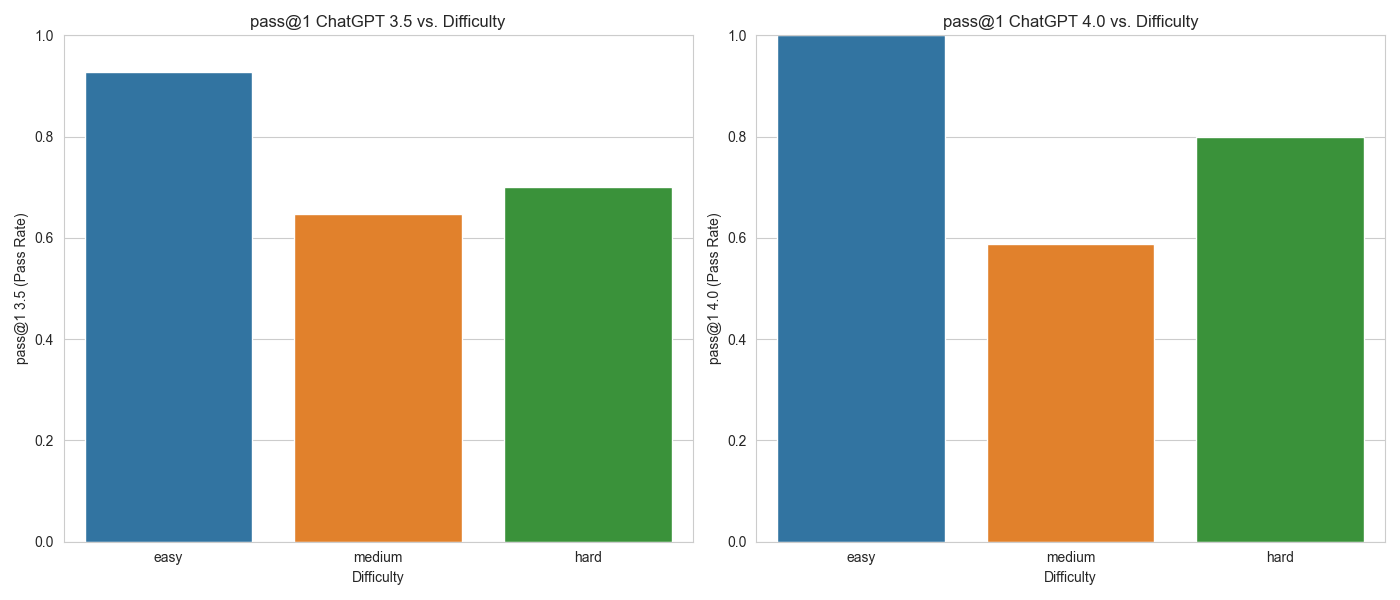
\includegraphics[width=\textwidth]{auswertung/passat1_difficulty}
        \caption{}
        \label{fig:1}
    \end{figure}

    Interessant ist allerdings zu sehen, dass ChatGPT 4.0 in der Kategorie "medium" sogar schlechtere Ergebnisse liefert als ChatGPT 3.5.

    Schaut man sich die Metrik "Anforderungen erfüllt" an und klammert die Programme aus, die grundsätzlich schon keinen korrekten Output liefern,
    zeigt sich, dass ChatGPT 3.5 in 6 von 32 Fällen die Anforderungen nicht erfüllt, wodurch tatsächlich nur noch 26 der 41 Aufgaben komplett richtig gelöst wurden.
    Das lässt sich vor allem auf die veralteten Daten zurückführen mit denen ChatGPT 3.5 trainiert wurde.
    In allen Fällen in denen ChatGPT 3.5 die Anforderungen nicht erfüllte aber eine richtige Ausgabe lieferte, handelte es sich um nicht
    verwendetes Pattern-Matching oder Datenklassen.
    Dass dennoch ein richtiger Output erzeugt wurde, liegt daran, dass ChatGPT 3.5 Pattern-Matching wie das vor dem
    Release dieser üblich war, mit if-, elif-, else-Verknüpfungen umsetzt.
    Betrachtet man die Lösungen von ChatGPT 4.0 unter denselben Bedingungen, kann man erkennen, dass ChatGPT 4.0 hier deutlich
    bessere Leistungen bringt als ChatGPT 3.5.
    Bei ChatGPT 4.0 erfüllen nämlich alle Programme, welche einen richtigen Output liefern auch die Anforderungen.
    Somit löst ChatGPT 4.0 mit 33 von 41 Aufgaben deutlich mehr Aufgaben korrekt als ChatGPT 3.5.
    Schaut man sich den Graphen aus Figure 4.1 nochmal an und bewertet die Programme nun anhand der Metrik "Anforderungen erfüllt" ergibt sich daraus der folgende Graph:
    \begin{figure}[H]
        \centering
        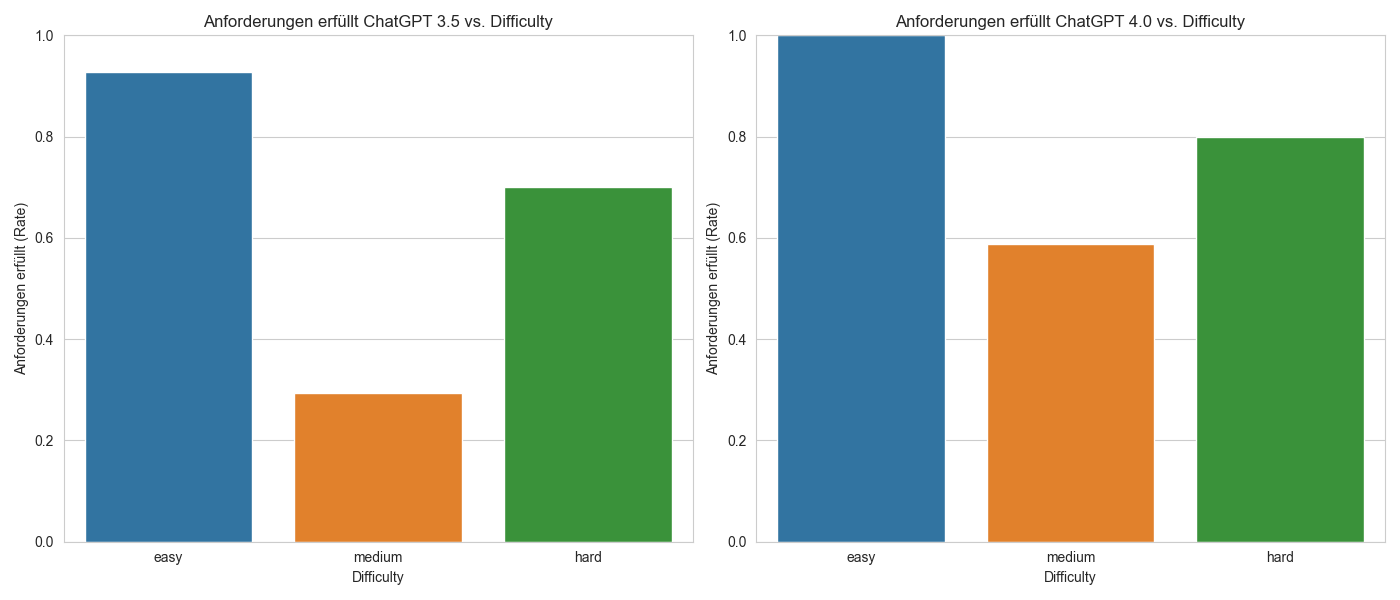
\includegraphics[width=\textwidth]{auswertung/req_met_difficulty}
        \caption{}
        \label{fig:2}
    \end{figure}


\section{Effizienz}
\label{sec:effizienz}
    Um die Effizienz der von ChatGPT generierten Programme zu bewerten ist es naheliegend sie mit den vom Lehrstuhl für
    Programmiersprachen bereitgestellten zu vergleichen.
    Die Metriken, die hierfür interessant sind, sind LOC$_{pars}$ und Cyclomatic Complexity, beziehungsweise McCabe Complexity.

    \subsection{LOC$_{pars}$}
    Vergleicht man die Zeilen an tatsächlichem Programmcode, also LOC$_{pars}$ mit denen von der jeweiligen Musterlösung,
    zeigt sich, dass ChatGPT 4.0 sogar etwas effizienter zu sein scheint als die Musterlösung, wärend ChatGPT 3.5 im Schnitt etwas weniger effizient ist.
    Wichtig zu beachten ist, dass die Fälle in denen ChatGPT 4.0 oder 3.5 jeweils nicht die Erwartungen erfüllt haben, nicht
    gewertet werden, da dies die Aussagekraft über die Effizienz anhand der Anzahl an Zeilen verfälschen würde.
    \begin{figure}[H]
        \centering
        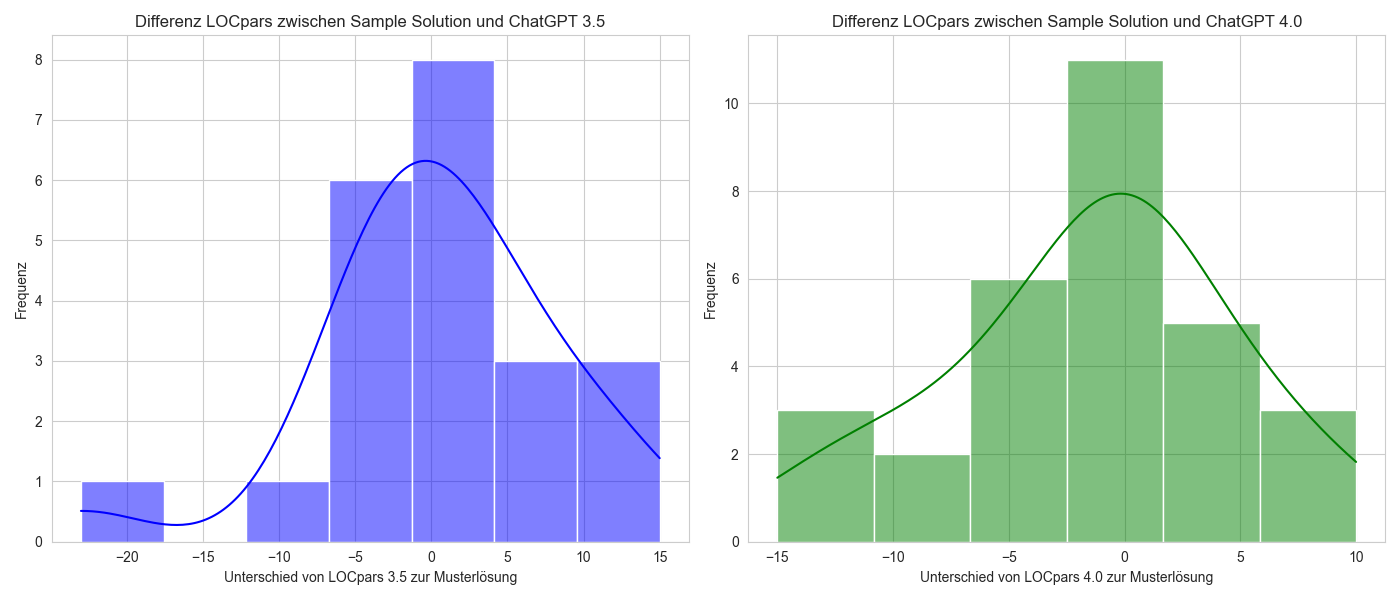
\includegraphics[width=\textwidth]{auswertung/locpars_vs_sample_solution}
        \caption{}
        \label{fig:3}
    \end{figure}
    Ist der Wert auf der x-Achse positiv, hat die jeweilige ChatGPT-Version mehr Zeilen gebraucht als die Musterlösung.
    Ist der Wert negativ, hat ChatGPT weniger LOC$_{pars}$ gebraucht um das Problem korrekt zu lösen.

    Im Groben lässt sich also sagen, dass ChatGPT gleich viele Zeilen braucht um die Aufgaben zu lösen wie die Musterlösung, wobei ChatGPT 4.0 sogar
    minimal weniger und ChatGPT 3.5 etwas mehr Zeilen braucht.
    Diese Metrik kann hilfreich sein, da Programme, die weniger Zeilen an Code haben, teils besser lesbar sind und weniger
    Leistung brauchen, es muss aber nicht zwangsweise heißen, dass ein Programm mit weniger Zeilen besser ist, als ein
    Programm für denselben Zweck mit mehr Zeilen.
    Dennoch ist es interessant die Zahlen gegenüberzustellen und zu vergleichen, da es durchaus im Interesse von Entwicklern ist,
    so wenig Code wie möglich zu schreiben.

    \subsection{Cyclomatic Comlexity}
    Bei der Cyclomatic Complexity handelt es sich, um ein sehr effizientes Mittel um die Effizienz eines Programms zu bewerten.
    Dadurch, dass mit jedem if, else, while usw. die Cyclomatic Complexity steigt, ist ein Programm, welches das gleiche
    Problem mit einer geringeren Cyclomatic Complexity lösen kann, als effizienter zu bewerten. Dies gilt nicht ausschließlich,
    lässt sich aber grob als Aussage treffen.

    Vergleicht man nun die Summe der Cyclomatic Complexity-Werte gruppiert nach der jeweiligen Schwierigkeit, fällt auf,
    fällt auf, dass sowohl ChatGPT 3.5 als auch ChatGPT 4.0 in der Summe weniger effiziente Programme schreiben.
    Nur beim Vergleich von ChatGPT 4.0 und der Musterlösung bei der Schwierigkeit hard, sind die Lösungen von ChatGPT 4.0
    etwas besser als die Musterlösung.
    \begin{figure}[H]
        \centering
        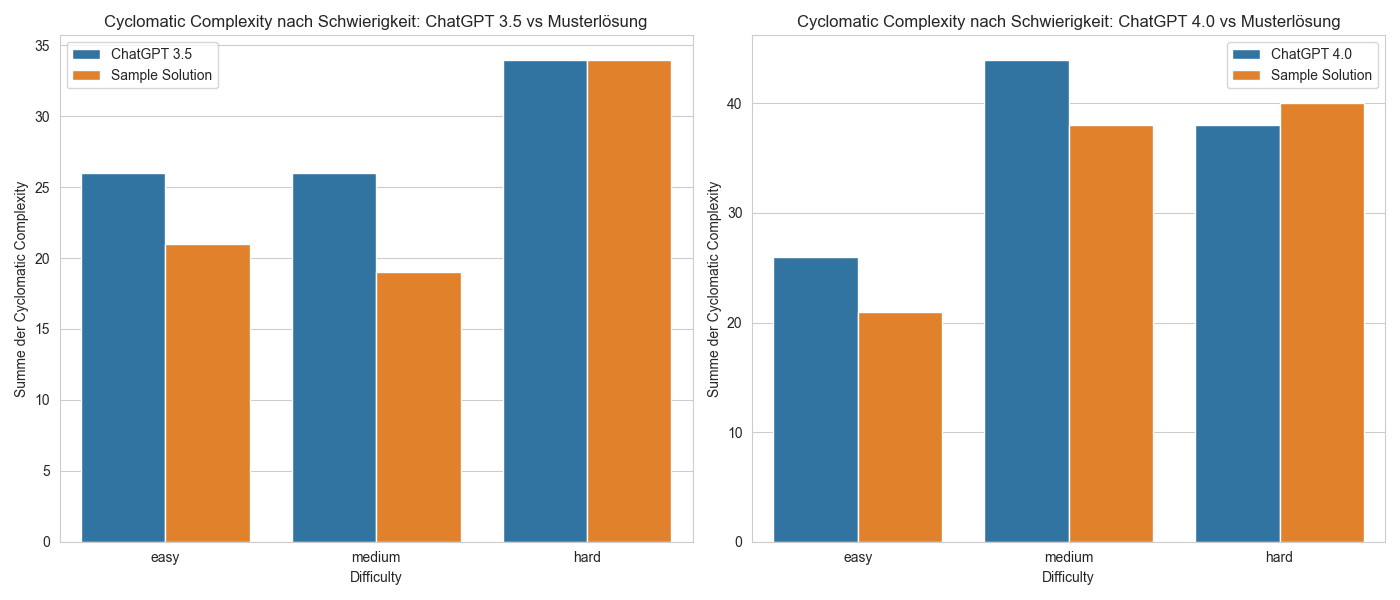
\includegraphics[width=\textwidth]{auswertung/cyclomatic_complexity}
        \caption{}
        \label{fig:4}
    \end{figure}
    Allerdings muss man auch sagen, dass der Abstand zur Musterlösung weder bei ChatGPT 3.5, noch bei ChatGPT 4.0 besonders
    hoch ist.
    Geht es allerdings darum die Programme besonders effizient zu gestalten, scheint ChatGPT nicht die beste Wahl zu sein.
    Das wird noch einmal deutlicher, wenn man berücksichtigt, dass die Musterlösungen des Lehrstuhls auch nicht darauf ausgelegt
    sind besonders effizient, sondern eher verständlich zu sein.
    Es ist also davon auszugehen, dass man die Probleme auch nochmal effizienter lösen könnte.

\ifstandalone
    \printglossary
    \printbibliography[heading=bibintoc]
\fi

\end{document}

    \documentclass[class=scrbook, crop=false]{standalone}
\usepackage[subpreambles=true]{standalone}
\ifstandalone
    % WARNING: Proceed with caution!

% -----------------------------------------------------------------------------------
% For package standalone
% -----------------------------------------------------------------------------------
\usepackage{import}

% -----------------------------------------------------------------------------------
% Language and typeset
% -----------------------------------------------------------------------------------
\usepackage[ngerman, english]{babel}

% Umlauts and other special characters (UTF-8)
% \usepackage[utf8]{inputenc}
\usepackage{fontspec}
\setsansfont{Arial}
% \usepackage[T1]{fontenc}  % Enable accented characters and umlauts
% LuaLatex doesn't need fontenc and uses UTF-8
% \usepackage{lmodern}  % Font face


% --------------------------------------------------------------------------------
% Page formatting
% --------------------------------------------------------------------------------
% Change the header/footer for chapter beginnings and normal pages
\usepackage[automark,headsepline]{scrlayer-scrpage}

% The package provides an easy and flexible user interface to customize the page
% layout, implementing auto-centering and auto-balancing mechanisms
% WARNING: WHEN CHANGING BCOR (Binding correction), the cover needs reworking!...
\newcommand{\theBCOR}{15mm}  % Define binding correction
\usepackage[
    bindingoffset=\theBCOR,
    % showframe, % Show boxes which indicate margins and paddings
    bottom = 3.5cm, % Margins
      left = 2.5cm,
     right = 2.5cm
] {geometry}

% The package 'float' provides a container for document objects which can not be
% broken over pages, such as tables and figures
% Needed for table and figure indexes  
\usepackage{float}

% support for landscape layout
\usepackage{lscape}

% support of \tablenotes command to add notes under table
\usepackage{threeparttable}

% To allow drawing more professional tables
\usepackage{booktabs}

% --------------------------------------------------------------------------------
% Contents
% --------------------------------------------------------------------------------
% Vector graphics (for Cover page)
\usepackage{tikz} 

% Allows additional parameters when including images
\usepackage{graphicx}

% Roman font family for all headings
\addtokomafont{disposition}{\rmfamily}

% Set the line spacing to 1.5
\usepackage[onehalfspacing]{setspace}

% Improves overall text spacing
% http://www.khirevich.com/latex/microtype/
\usepackage[stretch=10]{microtype}

% Math symbols like mu outside the math environment
\usepackage{textcomp}

% A comprehensive (SI) units package∗
% For defining SI units
\usepackage[
    range-units=single,         % Formatting ranges with single unit indication: 1 - 2 m
    range-phrase=-,             % Phrase for range: 1 - 2 m vs 1 to 2 m
    separate-uncertainty=true,  % sets +- between value and uncertainty 
    multi-part-units=repeat     % In expressions with multiple values (multi part numbers) 
                                % the unit is printed each time: 1 mm x 1 mm
] {siunitx}
% https://tex.stackexchange.com/questions/124488/multi-part-numbers-and-units-in-siunitx

% Allows Sourcecodes with highlighting 
\usepackage{listings}

% This package provides user control over the layout of the three basic list
% environments: enumerate, itemize and description
\usepackage{enumitem}
\setlist{nosep} % Remove the vertical space between \item elements in all lists

% ToDo Notes
% \setlength{\marginparwidth}{2cm}
\usepackage{todonotes}
\setuptodonotes{inline, inlinepar}
\reversemarginpar  % Put ToDo notes on the binding's side
% \usepackage{soul} % Colorful ToDo notes

% Check out colors here http://latexcolor.com/
\usepackage{xcolor}

\usepackage{amsmath}    % alignment of equations

% --------------------------------------------------------------------------------
% Other elements
% --------------------------------------------------------------------------------
% Blindtext: Organic looking text dummy
\usepackage{blindtext}

% Hyperlinks within the document (PDF)
% "hidelinks" hides visual highlighting of links
\usepackage[hidelinks]{hyperref}

% Package for Glossary and Index (Acronyms are listed in a separate list) 
\usepackage[acronym, nogroupskip]{glossaries} % groupskip: alphabetic grouping of entries

\usepackage{xltabular}   % <------- FOR glossaries

% Integration and management of bibliographies
\usepackage{csquotes}   % backend=biber in biblatex needs this package
\usepackage[
    style=ieee,   % style of the bibliography, entries are sorted in alphabetic order. "ieee" is another common style.
    backend=biber,      % based on package 'biber' 
    bibencoding=ascii   % ASCII Text encoding; may use "utf8" instead
] {biblatex}

% --------------------------------------------------------------------------------
%                               PATHS & FILES
% --------------------------------------------------------------------------------
% Fix paths for standalone compiling
\ifstandalone
    \def \home {..}
\else
    \def \home {.}
\fi

% Package: scrlayer-scrpage
% \def \stylePath {\home/settings+/style/page}
% Changing page style for header and footer
\automark{chapter}
\ihead{\leftmark}
\chead{}
\ohead{\thepage}
\ifoot*{}
\cfoot[\thepage]{}
\cfoot*{}
\ofoot*{}
\pagestyle{scrheadings}
  % Load page style

% Package: graphicx
\graphicspath{{\home/images/}}  % Set path to images

% Package: listings
% Change title for list of listings
\renewcommand\lstlistlistingname{\listoflistingstitle{}}

% Code highlighting for C++, you can also add others if needed
\lstset{
    language=C++,
    numbers=left,
    columns=fullflexible,
    aboveskip=5pt,
    belowskip=10pt,
    basicstyle=\small\ttfamily,
    backgroundcolor=\color{black!5},
    commentstyle=\color{darkgreen},
    keywordstyle=\color{blue},
    stringstyle=\color{gray},
    showspaces=false,
    showstringspaces=false,
    showtabs=false,
    xleftmargin=16pt,
    xrightmargin=0pt,
    framesep=5pt,
    framerule=3pt,
    frame=leftline,
    rulecolor=\color{steelblue},
    tabsize=2,
    breaklines=true,
    breakatwhitespace=true,
    prebreak={\mbox{$\hookleftarrow$}}
}
  % Set path to style file
\lstset{inputpath={\home/code/}} % Default path to code listings

% Package: glossaries

% NOT NEEDED? NO CHANGE???
% \glsenablehyper  % activates hyperlink from symbols and acronyms to glossary (symbols and acronyms list)




% Based on entry from Stackexchange
% https://tex.stackexchange.com/questions/269565/glossaries-how-to-customize-list-of-symbols-with-additional-column-for-units
%
% --------------------------------------------------------------------------------
% Style of the Symbols List
% --------------------------------------------------------------------------------
% Title of Symbols List
\newglossary[slg]{symbolslist}{syi}{syg}{\symbolslisttitle{}}

% Use addkey because we want three columns
% It's a mystery, but works 
\glsaddkey{unit}                    % new key
    {\glsentrytext{\glslabel}}      % entry text with default value
    {\glsentryunit}                 % commands which seem only to differ in the 
                                    % number of upper case letters
    {\GLsentryunit}
    {\glsunit}                      % command analogous to \glstext (function for 
                                    % link text (text produced by \gls{}), 
                                    % all lower case) 
    {\Glsunit}                      % command analogous to \Glstext (function for 
                                    % link text (text produced by \gls{}), 
                                    % first letter upper case)
    {\GLSunit}                      % command analogous to \GLStext (function for 
                                    % link text (text produced by \gls{}), all 
                                    % upper case)

\makeglossaries  % activate glossaries-package

\newglossarystyle{symbstyle} {
    \setglossarystyle{long3col}  % base this style on the list style
    \renewenvironment{theglossary} {
        % Change the table type --> 3 columns
        \xltabular{\linewidth}{p{0.2\textwidth}Xp{0.1\textwidth}}
    }{
        \endxltabular
    }

    %  Change the table header / footer
    \renewcommand*{\glossaryheader} {
        \bfseries \symbolslistname & \bfseries \symbolslistdescription & \bfseries \symbolslistunit \\
        \hline \endfirsthead
        \hline \endfoot
    }

    % Change the displayed items
    \renewcommand*{\glossentry}[2] {
        \glstarget{##1}{\glossentryname{##1}} & \glossentrydesc{##1} & \glsunit{##1} \\
        %               Symbol                      Description            Unit
    }
}  % Set path to symbols list style file
% Based on entry from Stackexchange
% https://tex.stackexchange.com/questions/269565/glossaries-how-to-customize-list-of-symbols-with-additional-column-for-units
%
% --------------------------------------------------------------------------------
% Style of the Acronyms List
% --------------------------------------------------------------------------------
\newglossarystyle{acrostyle} {
    %\setglossarystyle{long3col}   % base this style on the list style
    \renewenvironment{theglossary} {  % Change the table type --> 2 columns
        \xltabular{\linewidth}{p{0.2\textwidth}X}
    }{
        \endxltabular
    }

    % Change the table header
    \renewcommand*{\glossaryheader} {
        \bfseries \acronymstitle{} & \bfseries \acronymsdescription{} \\
        \hline
        \endfirsthead
        \hline\endfoot
    }

    % \renewcommand*{\glsgroupheading}[1]{}

    \renewcommand*{\glossaryentryfield}[5]{
        \glstarget{##1}{##2} & \glsentrydesc{##1}\\
    }

    % \renewcommand*{\glossarysubentryfield}[6]{ 
    %     &
    %     \glssubentryitem{##2} 
    %     \glstarget{##2}{\strut}##4 & ##6\\
    % }
 
    %*** GROUP SKIP *** 
    %\renewcommand*{\glsgroupskip}{&\\}% 
    %\renewcommand*{\glsgroupskip}{\addlinespace}% 
    %******************
}
  % Set path to acronym list style file
% -------------------------------------------------------------------------------
%               Listing of all Glossary and Acronym Entries 
%                           use as shown below
% -------------------------------------------------------------------------------

% ==== EXEMPLARY ENTRY FOR SYMBOLS LIST =========================================
\newglossaryentry{symb:Pi} {
    name=$\pi$,
    description=Geometrical value,
    unit=-,
    type=symbolslist
}

\newglossaryentry{symb:height} {
    name={$h$},
    description={Height},
    unit={\si{m}},
    type=symbolslist
}

\newglossaryentry{symb:energy} {
    name={$P$},
    description={Energy consumption},
    unit={\si{kW}},
    type={symbolslist}
}

\newglossaryentry{symb:A} {
    name=A,
    description=Geometrical value,
    unit=-,
    type=symbolslist
}

\newglossaryentry{symb:B} {
    name=B,
    description={Height},
    unit={\si{m}},
    type=symbolslist
}

\newglossaryentry{symb:C} {
    name=C,
    description={Energy consumption},
    unit={\si{kW}},
    type={symbolslist}
}

\newglossaryentry{symb:D} {
    name=D,
    description=Geometrical value,
    unit=-,
    type=symbolslist
}

\newglossaryentry{symb:E} {
    name=E,
    description={Height},
    unit={\si{m}},
    type=symbolslist
}

\newglossaryentry{symb:F} {
    name=F,
    description={Energy consumption},
    unit={\si{kW}},
    type={symbolslist}
}


\newglossaryentry{symb:G} {
    name=G,
    description=Geometrical value,
    unit=-,
    type=symbolslist
}

\newglossaryentry{symb:H} {
    name=H,
    description={Height},
    unit={\si{m}},
    type=symbolslist
}

\newglossaryentry{symb:I} {
    name=I,
    description={Energy consumption},
    unit={\si{kW}},
    type={symbolslist}
}

\newglossaryentry{symb:J} {
    name=J,
    description=Geometrical value,
    unit=-,
    type=symbolslist
}

\newglossaryentry{symb:K} {
    name=K,
    description={Height},
    unit={\si{m}},
    type=symbolslist
}

\newglossaryentry{symb:L} {
    name=L,
    description={Energy consumption},
    unit={\si{kW}},
    type={symbolslist}
}
\newglossaryentry{symb:M} {
    name=A,
    description=Geometrical value,
    unit=-,
    type=symbolslist
}

\newglossaryentry{symb:N} {
    name=B,
    description={Height},
    unit={\si{m}},
    type=symbolslist
}

\newglossaryentry{symb:O} {
    name=C,
    description={Energy consumption},
    unit={\si{kW}},
    type={symbolslist}
}

\newglossaryentry{symb:P} {
    name=D,
    description=Geometrical value,
    unit=-,
    type=symbolslist
}

\newglossaryentry{symb:Q} {
    name=E,
    description={Height},
    unit={\si{m}},
    type=symbolslist
}

\newglossaryentry{symb:R} {
    name=F,
    description={Energy consumption},
    unit={\si{kW}},
    type={symbolslist}
}


\newglossaryentry{symb:S} {
    name=G,
    description=Geometrical value,
    unit=-,
    type=symbolslist
}

\newglossaryentry{symb:T} {
    name=H,
    description={Height},
    unit={\si{m}},
    type=symbolslist
}

\newglossaryentry{symb:U} {
    name=I,
    description={Energy consumption},
    unit={\si{kW}},
    type={symbolslist}
}

\newglossaryentry{symb:V} {
    name=J,
    description=Geometrical value,
    unit=-,
    type=symbolslist
}

\newglossaryentry{symb:W} {
    name=K,
    description={Height},
    unit={\si{m}},
    type=symbolslist
}

\newglossaryentry{symb:X} {
    name=L,
    description={Energy consumption},
    unit={\si{kW}},
    type={symbolslist}
}

\newglossaryentry{symb:Y} {
    name=L,
    description={Energy consumption},
    unit={\si{kW}},
    type={symbolslist}
}

\newglossaryentry{symb:Z} {
    name=L,
    description={Energy consumption},
    unit={\si{kW}},
    type={symbolslist}
}

% ==== EXEMPLARY ENTRY FOR ACRONYMS LIST ========================================
% \newacronym{#label}{#acronym}{#long_form}

% define new command for custom arconym entry with only two arguments
% fabricates an easier way to use \newacronym 
\newcommand{\acroX}[2]{\newacronym{#1}{#1}{#2}}
% \acroX{label and arconym}{long name}
% \acroX{CD}               {Compact Disk}

\newcommand{\acroY}[3]{\newacronym{#1}{#2}{#3}}
% \arcoY{label}{acronym}{long name}
% \acroY{CD}   {cd}     {Compact Disk}
 
\newacronym{VRBD}  {VRBD}   {Violet-Red-Bile-Glucose-Agar}
\newacronym{lan}   {LAN}    {Local Area Network}
\newacronym{din}   {DIN}    {Deutsches Institut für Normung}
\newacronym{iso}   {ISO}    {Internationale Organisation für Normung}
\newacronym{sas}   {SAS}    {Serial Attached SCSI}
\newacronym{abbvz} {Abbvz.} {Abbildungsverzeichnis}
\newacronym{aA}    {VRBD}   {Violet-Red-Bile-Glucose-Agar}
\newacronym{aB}    {CD}     {Compact Disk}
\newacronym{aC}    {LAN}    {Local Area Network}
\newacronym{aD}    {DIN}    {Deutsches Institut für Normung}
\newacronym{aE}    {ISO}    {Internationale Organisation für Normung}
\newacronym{aF}    {SAS}    {Serial Attached SCSI}
\newacronym{aG}    {Abbvz.} {Abbildungsverzeichnis}
\newacronym{aH}    {VRBD}   {Violet-Red-Bile-Glucose-Agar}
\newacronym{aI}    {CD}     {Compact Disk}
\newacronym{aJ}    {LAN}    {Local Area Network}
\newacronym{aK}    {DIN}    {Deutsches Institut für Normung}
\newacronym{aL}    {ISO}    {Internationale Organisation für Normung}
\newacronym{aM}    {SAS}    {Serial Attached SCSI}
\newacronym{aN}    {Abbvz.} {Abbildungsverzeichnis}
\newacronym{aO}    {VRBD}   {Violet-Red-Bile-Glucose-Agar}
\newacronym{aP}    {CD}     {Compact Disk}
\newacronym{aQ}    {LAN}    {Local Area Network}
\newacronym{aR}    {DIN}    {Deutsches Institut für Normung}
\newacronym{aS}    {ISO}    {Internationale Organisation für Normung}
\newacronym{aT}    {SAS}    {Serial Attached SCSI}
\newacronym{aU}    {Abbvz.} {Abbildungsverzeichnis}
\newacronym{aV}    {CD}     {Compact Disk}
\newacronym{aW}    {LAN}    {Local Area Network}
\newacronym{aX}    {DIN}    {Deutsches Institut für Normung}
\newacronym{aY}    {ISO}    {Internationale Organisation für Normung}
\newacronym{aZ}    {SAS}    {Serial Attached SCSI}


% ==== EXEMPLARY ENTRY FOR MAIN GLOSSARY ========================================
    \newglossaryentry{Biofouling} {
        name=Biofouling,
        description={Some description}}
    
    \newglossaryentry{berlin} {
        name={Berlin},
        description={Berlin ist die Bundeshauptstadt der Bundesrepublik Deutschland und zugleich eines ihrer Länder. Die Stadt Berlin ist mit über 3,4 Millionen Einwohnern die bevölkerungsreichste und mit 892 Quadratkilometern die flächengrößte Gemeinde Deutschlands sowie nach Einwohnern die zweitgrößte der Europäischen Union. Sie bildet das Zentrum der Metropolregion Berlin/Brandenburg (6 Millionen Einw.) und der Agglomeration Berlin (4,4 Millionen Einw.). Der Stadtstaat unterteilt sich in zwölf Bezirke. Neben den Flüssen Spree und Havel befinden sich im Stadtgebiet kleinere Fließgewässer sowie zahlreiche Seen und Wälder}
        }
    \newglossaryentry{outsourcing} {
        name={Outsourcing},
        description={Outsourcing bzw. Auslagerung bezeichnet in der Ökonomie die Abgabe von Unternehmensaufgaben und -strukturen an externe oder interne Dienstleister. Es ist eine spezielle Form des Fremdbezugs von bisher intern erbrachter Leistung, wobei Verträge die Dauer und den Gegenstand der Leistung fixieren. Das grenzt Outsourcing von sonstigen Partnerschaften ab}
        }
    \newglossaryentry{asp} {
        name={Application Service Providing},
        description={Der Application Service Provider (Abkürzung ASP) bzw. Anwendungsdienstleister ist ein Dienstleister, der eine Anwendung (z. B. ein ERP-System) zum Informationsaustausch über ein öffentliches Netz (z. B. Internet) oder über ein privates Datennetz anbietet. Der ASP kümmert sich um die gesamte Administration, wie Datensicherung, das Einspielen von Patches usw. Anders als beim Applikations-Hosting ist Teil der ASP-Dienstleistung auch ein Service (z.B. Benutzerbetreuung) um die Anwendung herum}
        }
    % \newglossaryentry{policy}{name={Policy},description={Im geschäftlichen Bereich bezeichnet Policy eine interne Leit- bzw. Richtlinie, die formal durch das Unternehmen dokumentiert und über ihr Management verantwortet wird}}
    % \newglossaryentry{pcie}{name={PCI Express},description={PCI Express („Peripheral Component Interconnect Express“, abgekürzt PCIe oder PCI-E) ist ein Standard zur Verbindung von Peripheriegeräten mit dem Chipsatz eines Hauptprozessors. PCIe ist der Nachfolger von PCI, PCI-X und AGP und bietet im Vergleich zu seinen Vorgängern eine höhere Datenübertragungsrate pro Pin.}}
    % \newglossaryentry{realnumber}
  % Load glossary, symbol and acronyms list

% Package: biblatex
\addbibresource{\home/references/references.bib}  % Set path to bib resources

% Custom variables
\makeatletter
% ----------------------------------------------------------------------------
% Custom Colors (RGB 0-255, rgb 0-1)
% ----------------------------------------------------------------------------
\definecolor{dartmouthgreen}{rgb}{0.05, 0.5, 0.06}
\definecolor{myBlueFaded}{RGB}{80, 127, 186}
\definecolor{myBlue}{RGB}{42, 93, 156}

% Colors for code listings
\definecolor{darkgreen}{RGB}{0,100,0}
\definecolor{steelblue}{rgb}{0.27, 0.51, 0.71}

% ----------------------------------------------------------------------------
% Shorthands for custom colors and trademarks
% ----------------------------------------------------------------------------
\newcommand\red[1]{\textcolor{red}{\textbf{#1}}}
\newcommand\green[1]{\textcolor{dartmouthgreen}{#1}}
\newcommand\blue[1]{\textcolor{blue}{#1}}
\newcommand{\orange}[1]{{\color{orange}#1}}

% Quick access to business symbols via \TReg, \TCop and \TTra
\def\TReg{\textsuperscript{\tiny{\textregistered}}}
\def\TCop{\textsuperscript{\textcopyright}}
\def\TTra{\textsuperscript{\texttrademark}}

% ----------------------------------------------------------------------------
% Defining variables for cover pages and declaration of independence
% ----------------------------------------------------------------------------
% Author
\newcommand*{\matrikelnr}[1]{\gdef\@matrikelnr{#1}}

% University
\newcommand*{\uniEn}{University of Freiburg}
\newcommand*{\uni}{Albert-Ludwigs-Universität Freiburg}
\newcommand*{\institute}[1]{\gdef\@institute{#1}}
\newcommand*{\chair}[1]{\gdef\@chair{#1}}

% Thesis
\newcommand*{\thesisType}[1]{\gdef\@thesisType{#1}}
\newcommand*{\thesisTitle}[1]{\gdef\@thesisTitle{#1}}
\newcommand*{\submitDate}[1]{\gdef\@submitDate{#1}}
\newcommand*{\editingTime}[1]{\gdef\@editingTime{#1}}

% Examiners
\newcommand*{\firstExaminer}[1]{\gdef\@firstExaminer{#1}}
\newcommand*{\firstExaminerDepartment}[1]{\gdef\@firstExaminerDepartment{#1}}
\newcommand*{\firstExaminerChair}[1]{\gdef\@firstExaminerChair{#1}}
\newcommand*{\secondExaminer}[1]{\gdef\@secondExaminer{#1}}
\newcommand*{\secondExaminerDepartment}[1]{\gdef\@secondExaminerDepartment{#1}}
\newcommand*{\secondExaminerChair}[1]{\gdef\@secondExaminerChair{#1}}

% Supervisor
\newcommand*{\supervisor}[1]{\gdef\@supervisor{#1}}
\newcommand*{\supervisorDepartment}[1]{\gdef\@supervisorDepartment{#1}}
\newcommand*{\supervisorChair}[1]{\gdef\@supervisorChair{#1}}

% ----------------------------------------------------------------------------
% ToDo notes
% ----------------------------------------------------------------------------
% Let's fix up the ugly spacing of the 'todonotes' package
\renewcommand{\todo}[2][inline]{%
    \vspace{2mm}
    \@todo[#1]{#2}
    \vspace{-1mm}
}
\makeatother

% --------------------------------------------------------------------------------
%                                   OPTIONAL
% --------------------------------------------------------------------------------


% Simple arithmetic for LaTeX commands
% \usepackage{calc}

% Document Elements
% -------------------

% Index
% \usepackage{imakeidx}

% compact Lists
%\usepackage{paralist}

% visual improvements for citations
% \usepackage{epigraph}

% Create pseudo code
% https://www.overleaf.com/learn/latex/Algorithms
% \usepackage{algorithm}
% \usepackage{algorithmic}
%\usepackage[noend]{algpseudocode}

% Formatting
% -------------------
% Tweaks for scrbook, redefines commands of other packages
% \usepackage{scrhack}

% Intelligent space separator (nice for superscript?)
% \usepackage{xspace}

% Allows breaks within tables
%\usepackage{tabularx}

% Allows for page breaks in tables
% \usepackage{longtable}

% allows modifying of captions
% \usepackage{caption}

% Multiline comments
%\usepackage{verbatim}

% % Custom colors
% \definecolor{dartmouthgreen}{rgb}{0.05, 0.5, 0.06}

% IF you want to define unicode characters
% \DeclareUnicodeCharacter{0229}{\c{e}}
% \DeclareUnicodeCharacter{0306}{\u{Z}}


% Document elements
% ------------------------------------

% Table package
% \usepackage{booktabs}

% Pie diagram
% \usepackage{datapie}

% Side by Side images
% \usepackage{subcaption}

% For landscape tables
%\usepackage{pdflscape}
%\usepackage{afterpage}

% Graphics can be flow around by text
%\usepackage{wrapfig}

\fi

% ----------------------------------------------------------------------------
%                               Methods
% ----------------------------------------------------------------------------
\begin{document}

\chapter{Einschränkungen}
\label{ch:einschraenkungen}
    Diese Arbeit lässt auf jeden Fall Rückschlüsse darauf ziehen, wie gut ChatGPT in der jeweiligen Version im Generieren
    von Programmcode ist.
    Allerdings muss ganz klar darauf hingewiesen werden, dass der Datensatz mit 41 Aufgaben sehr klein ist und somit die Ergebnisse stark verfälscht sein können.
    Um noch präzisere Aussagen über die Effizienz und andere Metriken treffen zu können, braucht es einen Datensatz, der mindestens
    zehnmal so groß ist.
    Des Weiteren sind ein paar der Probleme die in den Aufgaben zu lösen waren klassische Programmierprobleme oder Aufgaben (zum Beispiel das Sierpinskidreieck).
    Bei diesen Aufgaben ist es durchaus möglich, dass ChatGPT bereits mit Lösungen zu Aufgaben dieser Art trainiert wurde
    und somit Aussagen darüber, wie gut ChatGPT im Allgemeinen im Programmieren ist, also auch im Bewältigen von neuen Aufgaben,
    zumindest mal mit vorsicht getroffen werden müssen.

\end{document}

    \documentclass[class=scrbook, crop=false]{standalone}
\usepackage[subpreambles=true]{standalone}
\ifstandalone
    % WARNING: Proceed with caution!

% -----------------------------------------------------------------------------------
% For package standalone
% -----------------------------------------------------------------------------------
\usepackage{import}

% -----------------------------------------------------------------------------------
% Language and typeset
% -----------------------------------------------------------------------------------
\usepackage[ngerman, english]{babel}

% Umlauts and other special characters (UTF-8)
% \usepackage[utf8]{inputenc}
\usepackage{fontspec}
\setsansfont{Arial}
% \usepackage[T1]{fontenc}  % Enable accented characters and umlauts
% LuaLatex doesn't need fontenc and uses UTF-8
% \usepackage{lmodern}  % Font face


% --------------------------------------------------------------------------------
% Page formatting
% --------------------------------------------------------------------------------
% Change the header/footer for chapter beginnings and normal pages
\usepackage[automark,headsepline]{scrlayer-scrpage}

% The package provides an easy and flexible user interface to customize the page
% layout, implementing auto-centering and auto-balancing mechanisms
% WARNING: WHEN CHANGING BCOR (Binding correction), the cover needs reworking!...
\newcommand{\theBCOR}{15mm}  % Define binding correction
\usepackage[
    bindingoffset=\theBCOR,
    % showframe, % Show boxes which indicate margins and paddings
    bottom = 3.5cm, % Margins
      left = 2.5cm,
     right = 2.5cm
] {geometry}

% The package 'float' provides a container for document objects which can not be
% broken over pages, such as tables and figures
% Needed for table and figure indexes  
\usepackage{float}

% support for landscape layout
\usepackage{lscape}

% support of \tablenotes command to add notes under table
\usepackage{threeparttable}

% To allow drawing more professional tables
\usepackage{booktabs}

% --------------------------------------------------------------------------------
% Contents
% --------------------------------------------------------------------------------
% Vector graphics (for Cover page)
\usepackage{tikz} 

% Allows additional parameters when including images
\usepackage{graphicx}

% Roman font family for all headings
\addtokomafont{disposition}{\rmfamily}

% Set the line spacing to 1.5
\usepackage[onehalfspacing]{setspace}

% Improves overall text spacing
% http://www.khirevich.com/latex/microtype/
\usepackage[stretch=10]{microtype}

% Math symbols like mu outside the math environment
\usepackage{textcomp}

% A comprehensive (SI) units package∗
% For defining SI units
\usepackage[
    range-units=single,         % Formatting ranges with single unit indication: 1 - 2 m
    range-phrase=-,             % Phrase for range: 1 - 2 m vs 1 to 2 m
    separate-uncertainty=true,  % sets +- between value and uncertainty 
    multi-part-units=repeat     % In expressions with multiple values (multi part numbers) 
                                % the unit is printed each time: 1 mm x 1 mm
] {siunitx}
% https://tex.stackexchange.com/questions/124488/multi-part-numbers-and-units-in-siunitx

% Allows Sourcecodes with highlighting 
\usepackage{listings}

% This package provides user control over the layout of the three basic list
% environments: enumerate, itemize and description
\usepackage{enumitem}
\setlist{nosep} % Remove the vertical space between \item elements in all lists

% ToDo Notes
% \setlength{\marginparwidth}{2cm}
\usepackage{todonotes}
\setuptodonotes{inline, inlinepar}
\reversemarginpar  % Put ToDo notes on the binding's side
% \usepackage{soul} % Colorful ToDo notes

% Check out colors here http://latexcolor.com/
\usepackage{xcolor}

\usepackage{amsmath}    % alignment of equations

% --------------------------------------------------------------------------------
% Other elements
% --------------------------------------------------------------------------------
% Blindtext: Organic looking text dummy
\usepackage{blindtext}

% Hyperlinks within the document (PDF)
% "hidelinks" hides visual highlighting of links
\usepackage[hidelinks]{hyperref}

% Package for Glossary and Index (Acronyms are listed in a separate list) 
\usepackage[acronym, nogroupskip]{glossaries} % groupskip: alphabetic grouping of entries

\usepackage{xltabular}   % <------- FOR glossaries

% Integration and management of bibliographies
\usepackage{csquotes}   % backend=biber in biblatex needs this package
\usepackage[
    style=ieee,   % style of the bibliography, entries are sorted in alphabetic order. "ieee" is another common style.
    backend=biber,      % based on package 'biber' 
    bibencoding=ascii   % ASCII Text encoding; may use "utf8" instead
] {biblatex}

% --------------------------------------------------------------------------------
%                               PATHS & FILES
% --------------------------------------------------------------------------------
% Fix paths for standalone compiling
\ifstandalone
    \def \home {..}
\else
    \def \home {.}
\fi

% Package: scrlayer-scrpage
% \def \stylePath {\home/settings+/style/page}
% Changing page style for header and footer
\automark{chapter}
\ihead{\leftmark}
\chead{}
\ohead{\thepage}
\ifoot*{}
\cfoot[\thepage]{}
\cfoot*{}
\ofoot*{}
\pagestyle{scrheadings}
  % Load page style

% Package: graphicx
\graphicspath{{\home/images/}}  % Set path to images

% Package: listings
% Change title for list of listings
\renewcommand\lstlistlistingname{\listoflistingstitle{}}

% Code highlighting for C++, you can also add others if needed
\lstset{
    language=C++,
    numbers=left,
    columns=fullflexible,
    aboveskip=5pt,
    belowskip=10pt,
    basicstyle=\small\ttfamily,
    backgroundcolor=\color{black!5},
    commentstyle=\color{darkgreen},
    keywordstyle=\color{blue},
    stringstyle=\color{gray},
    showspaces=false,
    showstringspaces=false,
    showtabs=false,
    xleftmargin=16pt,
    xrightmargin=0pt,
    framesep=5pt,
    framerule=3pt,
    frame=leftline,
    rulecolor=\color{steelblue},
    tabsize=2,
    breaklines=true,
    breakatwhitespace=true,
    prebreak={\mbox{$\hookleftarrow$}}
}
  % Set path to style file
\lstset{inputpath={\home/code/}} % Default path to code listings

% Package: glossaries

% NOT NEEDED? NO CHANGE???
% \glsenablehyper  % activates hyperlink from symbols and acronyms to glossary (symbols and acronyms list)




% Based on entry from Stackexchange
% https://tex.stackexchange.com/questions/269565/glossaries-how-to-customize-list-of-symbols-with-additional-column-for-units
%
% --------------------------------------------------------------------------------
% Style of the Symbols List
% --------------------------------------------------------------------------------
% Title of Symbols List
\newglossary[slg]{symbolslist}{syi}{syg}{\symbolslisttitle{}}

% Use addkey because we want three columns
% It's a mystery, but works 
\glsaddkey{unit}                    % new key
    {\glsentrytext{\glslabel}}      % entry text with default value
    {\glsentryunit}                 % commands which seem only to differ in the 
                                    % number of upper case letters
    {\GLsentryunit}
    {\glsunit}                      % command analogous to \glstext (function for 
                                    % link text (text produced by \gls{}), 
                                    % all lower case) 
    {\Glsunit}                      % command analogous to \Glstext (function for 
                                    % link text (text produced by \gls{}), 
                                    % first letter upper case)
    {\GLSunit}                      % command analogous to \GLStext (function for 
                                    % link text (text produced by \gls{}), all 
                                    % upper case)

\makeglossaries  % activate glossaries-package

\newglossarystyle{symbstyle} {
    \setglossarystyle{long3col}  % base this style on the list style
    \renewenvironment{theglossary} {
        % Change the table type --> 3 columns
        \xltabular{\linewidth}{p{0.2\textwidth}Xp{0.1\textwidth}}
    }{
        \endxltabular
    }

    %  Change the table header / footer
    \renewcommand*{\glossaryheader} {
        \bfseries \symbolslistname & \bfseries \symbolslistdescription & \bfseries \symbolslistunit \\
        \hline \endfirsthead
        \hline \endfoot
    }

    % Change the displayed items
    \renewcommand*{\glossentry}[2] {
        \glstarget{##1}{\glossentryname{##1}} & \glossentrydesc{##1} & \glsunit{##1} \\
        %               Symbol                      Description            Unit
    }
}  % Set path to symbols list style file
% Based on entry from Stackexchange
% https://tex.stackexchange.com/questions/269565/glossaries-how-to-customize-list-of-symbols-with-additional-column-for-units
%
% --------------------------------------------------------------------------------
% Style of the Acronyms List
% --------------------------------------------------------------------------------
\newglossarystyle{acrostyle} {
    %\setglossarystyle{long3col}   % base this style on the list style
    \renewenvironment{theglossary} {  % Change the table type --> 2 columns
        \xltabular{\linewidth}{p{0.2\textwidth}X}
    }{
        \endxltabular
    }

    % Change the table header
    \renewcommand*{\glossaryheader} {
        \bfseries \acronymstitle{} & \bfseries \acronymsdescription{} \\
        \hline
        \endfirsthead
        \hline\endfoot
    }

    % \renewcommand*{\glsgroupheading}[1]{}

    \renewcommand*{\glossaryentryfield}[5]{
        \glstarget{##1}{##2} & \glsentrydesc{##1}\\
    }

    % \renewcommand*{\glossarysubentryfield}[6]{ 
    %     &
    %     \glssubentryitem{##2} 
    %     \glstarget{##2}{\strut}##4 & ##6\\
    % }
 
    %*** GROUP SKIP *** 
    %\renewcommand*{\glsgroupskip}{&\\}% 
    %\renewcommand*{\glsgroupskip}{\addlinespace}% 
    %******************
}
  % Set path to acronym list style file
% -------------------------------------------------------------------------------
%               Listing of all Glossary and Acronym Entries 
%                           use as shown below
% -------------------------------------------------------------------------------

% ==== EXEMPLARY ENTRY FOR SYMBOLS LIST =========================================
\newglossaryentry{symb:Pi} {
    name=$\pi$,
    description=Geometrical value,
    unit=-,
    type=symbolslist
}

\newglossaryentry{symb:height} {
    name={$h$},
    description={Height},
    unit={\si{m}},
    type=symbolslist
}

\newglossaryentry{symb:energy} {
    name={$P$},
    description={Energy consumption},
    unit={\si{kW}},
    type={symbolslist}
}

\newglossaryentry{symb:A} {
    name=A,
    description=Geometrical value,
    unit=-,
    type=symbolslist
}

\newglossaryentry{symb:B} {
    name=B,
    description={Height},
    unit={\si{m}},
    type=symbolslist
}

\newglossaryentry{symb:C} {
    name=C,
    description={Energy consumption},
    unit={\si{kW}},
    type={symbolslist}
}

\newglossaryentry{symb:D} {
    name=D,
    description=Geometrical value,
    unit=-,
    type=symbolslist
}

\newglossaryentry{symb:E} {
    name=E,
    description={Height},
    unit={\si{m}},
    type=symbolslist
}

\newglossaryentry{symb:F} {
    name=F,
    description={Energy consumption},
    unit={\si{kW}},
    type={symbolslist}
}


\newglossaryentry{symb:G} {
    name=G,
    description=Geometrical value,
    unit=-,
    type=symbolslist
}

\newglossaryentry{symb:H} {
    name=H,
    description={Height},
    unit={\si{m}},
    type=symbolslist
}

\newglossaryentry{symb:I} {
    name=I,
    description={Energy consumption},
    unit={\si{kW}},
    type={symbolslist}
}

\newglossaryentry{symb:J} {
    name=J,
    description=Geometrical value,
    unit=-,
    type=symbolslist
}

\newglossaryentry{symb:K} {
    name=K,
    description={Height},
    unit={\si{m}},
    type=symbolslist
}

\newglossaryentry{symb:L} {
    name=L,
    description={Energy consumption},
    unit={\si{kW}},
    type={symbolslist}
}
\newglossaryentry{symb:M} {
    name=A,
    description=Geometrical value,
    unit=-,
    type=symbolslist
}

\newglossaryentry{symb:N} {
    name=B,
    description={Height},
    unit={\si{m}},
    type=symbolslist
}

\newglossaryentry{symb:O} {
    name=C,
    description={Energy consumption},
    unit={\si{kW}},
    type={symbolslist}
}

\newglossaryentry{symb:P} {
    name=D,
    description=Geometrical value,
    unit=-,
    type=symbolslist
}

\newglossaryentry{symb:Q} {
    name=E,
    description={Height},
    unit={\si{m}},
    type=symbolslist
}

\newglossaryentry{symb:R} {
    name=F,
    description={Energy consumption},
    unit={\si{kW}},
    type={symbolslist}
}


\newglossaryentry{symb:S} {
    name=G,
    description=Geometrical value,
    unit=-,
    type=symbolslist
}

\newglossaryentry{symb:T} {
    name=H,
    description={Height},
    unit={\si{m}},
    type=symbolslist
}

\newglossaryentry{symb:U} {
    name=I,
    description={Energy consumption},
    unit={\si{kW}},
    type={symbolslist}
}

\newglossaryentry{symb:V} {
    name=J,
    description=Geometrical value,
    unit=-,
    type=symbolslist
}

\newglossaryentry{symb:W} {
    name=K,
    description={Height},
    unit={\si{m}},
    type=symbolslist
}

\newglossaryentry{symb:X} {
    name=L,
    description={Energy consumption},
    unit={\si{kW}},
    type={symbolslist}
}

\newglossaryentry{symb:Y} {
    name=L,
    description={Energy consumption},
    unit={\si{kW}},
    type={symbolslist}
}

\newglossaryentry{symb:Z} {
    name=L,
    description={Energy consumption},
    unit={\si{kW}},
    type={symbolslist}
}

% ==== EXEMPLARY ENTRY FOR ACRONYMS LIST ========================================
% \newacronym{#label}{#acronym}{#long_form}

% define new command for custom arconym entry with only two arguments
% fabricates an easier way to use \newacronym 
\newcommand{\acroX}[2]{\newacronym{#1}{#1}{#2}}
% \acroX{label and arconym}{long name}
% \acroX{CD}               {Compact Disk}

\newcommand{\acroY}[3]{\newacronym{#1}{#2}{#3}}
% \arcoY{label}{acronym}{long name}
% \acroY{CD}   {cd}     {Compact Disk}
 
\newacronym{VRBD}  {VRBD}   {Violet-Red-Bile-Glucose-Agar}
\newacronym{lan}   {LAN}    {Local Area Network}
\newacronym{din}   {DIN}    {Deutsches Institut für Normung}
\newacronym{iso}   {ISO}    {Internationale Organisation für Normung}
\newacronym{sas}   {SAS}    {Serial Attached SCSI}
\newacronym{abbvz} {Abbvz.} {Abbildungsverzeichnis}
\newacronym{aA}    {VRBD}   {Violet-Red-Bile-Glucose-Agar}
\newacronym{aB}    {CD}     {Compact Disk}
\newacronym{aC}    {LAN}    {Local Area Network}
\newacronym{aD}    {DIN}    {Deutsches Institut für Normung}
\newacronym{aE}    {ISO}    {Internationale Organisation für Normung}
\newacronym{aF}    {SAS}    {Serial Attached SCSI}
\newacronym{aG}    {Abbvz.} {Abbildungsverzeichnis}
\newacronym{aH}    {VRBD}   {Violet-Red-Bile-Glucose-Agar}
\newacronym{aI}    {CD}     {Compact Disk}
\newacronym{aJ}    {LAN}    {Local Area Network}
\newacronym{aK}    {DIN}    {Deutsches Institut für Normung}
\newacronym{aL}    {ISO}    {Internationale Organisation für Normung}
\newacronym{aM}    {SAS}    {Serial Attached SCSI}
\newacronym{aN}    {Abbvz.} {Abbildungsverzeichnis}
\newacronym{aO}    {VRBD}   {Violet-Red-Bile-Glucose-Agar}
\newacronym{aP}    {CD}     {Compact Disk}
\newacronym{aQ}    {LAN}    {Local Area Network}
\newacronym{aR}    {DIN}    {Deutsches Institut für Normung}
\newacronym{aS}    {ISO}    {Internationale Organisation für Normung}
\newacronym{aT}    {SAS}    {Serial Attached SCSI}
\newacronym{aU}    {Abbvz.} {Abbildungsverzeichnis}
\newacronym{aV}    {CD}     {Compact Disk}
\newacronym{aW}    {LAN}    {Local Area Network}
\newacronym{aX}    {DIN}    {Deutsches Institut für Normung}
\newacronym{aY}    {ISO}    {Internationale Organisation für Normung}
\newacronym{aZ}    {SAS}    {Serial Attached SCSI}


% ==== EXEMPLARY ENTRY FOR MAIN GLOSSARY ========================================
    \newglossaryentry{Biofouling} {
        name=Biofouling,
        description={Some description}}
    
    \newglossaryentry{berlin} {
        name={Berlin},
        description={Berlin ist die Bundeshauptstadt der Bundesrepublik Deutschland und zugleich eines ihrer Länder. Die Stadt Berlin ist mit über 3,4 Millionen Einwohnern die bevölkerungsreichste und mit 892 Quadratkilometern die flächengrößte Gemeinde Deutschlands sowie nach Einwohnern die zweitgrößte der Europäischen Union. Sie bildet das Zentrum der Metropolregion Berlin/Brandenburg (6 Millionen Einw.) und der Agglomeration Berlin (4,4 Millionen Einw.). Der Stadtstaat unterteilt sich in zwölf Bezirke. Neben den Flüssen Spree und Havel befinden sich im Stadtgebiet kleinere Fließgewässer sowie zahlreiche Seen und Wälder}
        }
    \newglossaryentry{outsourcing} {
        name={Outsourcing},
        description={Outsourcing bzw. Auslagerung bezeichnet in der Ökonomie die Abgabe von Unternehmensaufgaben und -strukturen an externe oder interne Dienstleister. Es ist eine spezielle Form des Fremdbezugs von bisher intern erbrachter Leistung, wobei Verträge die Dauer und den Gegenstand der Leistung fixieren. Das grenzt Outsourcing von sonstigen Partnerschaften ab}
        }
    \newglossaryentry{asp} {
        name={Application Service Providing},
        description={Der Application Service Provider (Abkürzung ASP) bzw. Anwendungsdienstleister ist ein Dienstleister, der eine Anwendung (z. B. ein ERP-System) zum Informationsaustausch über ein öffentliches Netz (z. B. Internet) oder über ein privates Datennetz anbietet. Der ASP kümmert sich um die gesamte Administration, wie Datensicherung, das Einspielen von Patches usw. Anders als beim Applikations-Hosting ist Teil der ASP-Dienstleistung auch ein Service (z.B. Benutzerbetreuung) um die Anwendung herum}
        }
    % \newglossaryentry{policy}{name={Policy},description={Im geschäftlichen Bereich bezeichnet Policy eine interne Leit- bzw. Richtlinie, die formal durch das Unternehmen dokumentiert und über ihr Management verantwortet wird}}
    % \newglossaryentry{pcie}{name={PCI Express},description={PCI Express („Peripheral Component Interconnect Express“, abgekürzt PCIe oder PCI-E) ist ein Standard zur Verbindung von Peripheriegeräten mit dem Chipsatz eines Hauptprozessors. PCIe ist der Nachfolger von PCI, PCI-X und AGP und bietet im Vergleich zu seinen Vorgängern eine höhere Datenübertragungsrate pro Pin.}}
    % \newglossaryentry{realnumber}
  % Load glossary, symbol and acronyms list

% Package: biblatex
\addbibresource{\home/references/references.bib}  % Set path to bib resources

% Custom variables
\makeatletter
% ----------------------------------------------------------------------------
% Custom Colors (RGB 0-255, rgb 0-1)
% ----------------------------------------------------------------------------
\definecolor{dartmouthgreen}{rgb}{0.05, 0.5, 0.06}
\definecolor{myBlueFaded}{RGB}{80, 127, 186}
\definecolor{myBlue}{RGB}{42, 93, 156}

% Colors for code listings
\definecolor{darkgreen}{RGB}{0,100,0}
\definecolor{steelblue}{rgb}{0.27, 0.51, 0.71}

% ----------------------------------------------------------------------------
% Shorthands for custom colors and trademarks
% ----------------------------------------------------------------------------
\newcommand\red[1]{\textcolor{red}{\textbf{#1}}}
\newcommand\green[1]{\textcolor{dartmouthgreen}{#1}}
\newcommand\blue[1]{\textcolor{blue}{#1}}
\newcommand{\orange}[1]{{\color{orange}#1}}

% Quick access to business symbols via \TReg, \TCop and \TTra
\def\TReg{\textsuperscript{\tiny{\textregistered}}}
\def\TCop{\textsuperscript{\textcopyright}}
\def\TTra{\textsuperscript{\texttrademark}}

% ----------------------------------------------------------------------------
% Defining variables for cover pages and declaration of independence
% ----------------------------------------------------------------------------
% Author
\newcommand*{\matrikelnr}[1]{\gdef\@matrikelnr{#1}}

% University
\newcommand*{\uniEn}{University of Freiburg}
\newcommand*{\uni}{Albert-Ludwigs-Universität Freiburg}
\newcommand*{\institute}[1]{\gdef\@institute{#1}}
\newcommand*{\chair}[1]{\gdef\@chair{#1}}

% Thesis
\newcommand*{\thesisType}[1]{\gdef\@thesisType{#1}}
\newcommand*{\thesisTitle}[1]{\gdef\@thesisTitle{#1}}
\newcommand*{\submitDate}[1]{\gdef\@submitDate{#1}}
\newcommand*{\editingTime}[1]{\gdef\@editingTime{#1}}

% Examiners
\newcommand*{\firstExaminer}[1]{\gdef\@firstExaminer{#1}}
\newcommand*{\firstExaminerDepartment}[1]{\gdef\@firstExaminerDepartment{#1}}
\newcommand*{\firstExaminerChair}[1]{\gdef\@firstExaminerChair{#1}}
\newcommand*{\secondExaminer}[1]{\gdef\@secondExaminer{#1}}
\newcommand*{\secondExaminerDepartment}[1]{\gdef\@secondExaminerDepartment{#1}}
\newcommand*{\secondExaminerChair}[1]{\gdef\@secondExaminerChair{#1}}

% Supervisor
\newcommand*{\supervisor}[1]{\gdef\@supervisor{#1}}
\newcommand*{\supervisorDepartment}[1]{\gdef\@supervisorDepartment{#1}}
\newcommand*{\supervisorChair}[1]{\gdef\@supervisorChair{#1}}

% ----------------------------------------------------------------------------
% ToDo notes
% ----------------------------------------------------------------------------
% Let's fix up the ugly spacing of the 'todonotes' package
\renewcommand{\todo}[2][inline]{%
    \vspace{2mm}
    \@todo[#1]{#2}
    \vspace{-1mm}
}
\makeatother

% --------------------------------------------------------------------------------
%                                   OPTIONAL
% --------------------------------------------------------------------------------


% Simple arithmetic for LaTeX commands
% \usepackage{calc}

% Document Elements
% -------------------

% Index
% \usepackage{imakeidx}

% compact Lists
%\usepackage{paralist}

% visual improvements for citations
% \usepackage{epigraph}

% Create pseudo code
% https://www.overleaf.com/learn/latex/Algorithms
% \usepackage{algorithm}
% \usepackage{algorithmic}
%\usepackage[noend]{algpseudocode}

% Formatting
% -------------------
% Tweaks for scrbook, redefines commands of other packages
% \usepackage{scrhack}

% Intelligent space separator (nice for superscript?)
% \usepackage{xspace}

% Allows breaks within tables
%\usepackage{tabularx}

% Allows for page breaks in tables
% \usepackage{longtable}

% allows modifying of captions
% \usepackage{caption}

% Multiline comments
%\usepackage{verbatim}

% % Custom colors
% \definecolor{dartmouthgreen}{rgb}{0.05, 0.5, 0.06}

% IF you want to define unicode characters
% \DeclareUnicodeCharacter{0229}{\c{e}}
% \DeclareUnicodeCharacter{0306}{\u{Z}}


% Document elements
% ------------------------------------

% Table package
% \usepackage{booktabs}

% Pie diagram
% \usepackage{datapie}

% Side by Side images
% \usepackage{subcaption}

% For landscape tables
%\usepackage{pdflscape}
%\usepackage{afterpage}

% Graphics can be flow around by text
%\usepackage{wrapfig}

\fi

% ----------------------------------------------------------------------------
%                               Zusammenfassung
% ----------------------------------------------------------------------------
\begin{document}

\chapter{Zusammenfassung}
\label{ch:zusammenfassung}
    ChatGPT kann immer mehr und ist im Umgang mit Programmieraufgaben durchaus ein brauchbares Werkzeug.
    Allerdings ist ChatGPT zum aktuellen Stand noch nicht uneingeschränkt zum Programmieren nutzbar.
    Gerade, wenn man die kostenfreie Version nutzt, muss man sich darüber im Klaren sein, dass diese bestimmte Anforderungen einfach nicht erfüllen kann.
    Und auch im Allgemeinen zeigt sich, dass man derzeit nach wie vor über eigene Programmierfähigkeiten verfügen muss,
    wenn man ChatGPT zum Programmieren verwenden will.
    Der generierte Code ist nicht zwangsweise fehlerfrei und wenn man nicht gerade eine Musterlösung mit dem korrekten
    Output zur Hand hat, kann es durchaus vorkommen, dass Werte als vermeintlich richtig berechnet angesehen werden,
    obwohl sie das gar nicht sind.
    Das ist insbesondere bei sicherheitskritischen Programmen ein großes Problem, weshalb gerade hier ChatGPT definitv
    noch nicht eingesetzt werden kann.
    Auch wenn man besonders effizienten Programmcode erwartet, wird man bei ChatGPT nicht fündig werden und es mag sich
    mehr lohnen, sich an einen erfahrenen Entwickler zu wenden.
    Vergleicht man aber ChatGPT mit Informatik Studierenden im ersten Semester, so ist ChatGPT keineswegs ein schlechtes Werkzeug
    und kann durchaus mit Menschen mithalten.
    Wenn man berücksichtigt, was die Entwicklung von KI der letzten Jahre mit sich gebracht hat, ist da aber vermutlich
    noch viel Luft nach oben und das Potenzial ist noch lange nicht ausgeschöpft.
    Aus diesem Grund ist es auch interessant, Arbeiten wie diese in regelmäßigen Abständen zu wiederholen um, die
    Entwicklung von ChatGPT festhalten zu können.

\end{document}

    \documentclass[class=scrbook, crop=false]{standalone}
\usepackage{lstdoc}
\ifstandalone
    % WARNING: Proceed with caution!

% -----------------------------------------------------------------------------------
% For package standalone
% -----------------------------------------------------------------------------------
\usepackage{import}

% -----------------------------------------------------------------------------------
% Language and typeset
% -----------------------------------------------------------------------------------
\usepackage[ngerman, english]{babel}

% Umlauts and other special characters (UTF-8)
% \usepackage[utf8]{inputenc}
\usepackage{fontspec}
\setsansfont{Arial}
% \usepackage[T1]{fontenc}  % Enable accented characters and umlauts
% LuaLatex doesn't need fontenc and uses UTF-8
% \usepackage{lmodern}  % Font face


% --------------------------------------------------------------------------------
% Page formatting
% --------------------------------------------------------------------------------
% Change the header/footer for chapter beginnings and normal pages
\usepackage[automark,headsepline]{scrlayer-scrpage}

% The package provides an easy and flexible user interface to customize the page
% layout, implementing auto-centering and auto-balancing mechanisms
% WARNING: WHEN CHANGING BCOR (Binding correction), the cover needs reworking!...
\newcommand{\theBCOR}{15mm}  % Define binding correction
\usepackage[
    bindingoffset=\theBCOR,
    % showframe, % Show boxes which indicate margins and paddings
    bottom = 3.5cm, % Margins
      left = 2.5cm,
     right = 2.5cm
] {geometry}

% The package 'float' provides a container for document objects which can not be
% broken over pages, such as tables and figures
% Needed for table and figure indexes  
\usepackage{float}

% support for landscape layout
\usepackage{lscape}

% support of \tablenotes command to add notes under table
\usepackage{threeparttable}

% To allow drawing more professional tables
\usepackage{booktabs}

% --------------------------------------------------------------------------------
% Contents
% --------------------------------------------------------------------------------
% Vector graphics (for Cover page)
\usepackage{tikz} 

% Allows additional parameters when including images
\usepackage{graphicx}

% Roman font family for all headings
\addtokomafont{disposition}{\rmfamily}

% Set the line spacing to 1.5
\usepackage[onehalfspacing]{setspace}

% Improves overall text spacing
% http://www.khirevich.com/latex/microtype/
\usepackage[stretch=10]{microtype}

% Math symbols like mu outside the math environment
\usepackage{textcomp}

% A comprehensive (SI) units package∗
% For defining SI units
\usepackage[
    range-units=single,         % Formatting ranges with single unit indication: 1 - 2 m
    range-phrase=-,             % Phrase for range: 1 - 2 m vs 1 to 2 m
    separate-uncertainty=true,  % sets +- between value and uncertainty 
    multi-part-units=repeat     % In expressions with multiple values (multi part numbers) 
                                % the unit is printed each time: 1 mm x 1 mm
] {siunitx}
% https://tex.stackexchange.com/questions/124488/multi-part-numbers-and-units-in-siunitx

% Allows Sourcecodes with highlighting 
\usepackage{listings}

% This package provides user control over the layout of the three basic list
% environments: enumerate, itemize and description
\usepackage{enumitem}
\setlist{nosep} % Remove the vertical space between \item elements in all lists

% ToDo Notes
% \setlength{\marginparwidth}{2cm}
\usepackage{todonotes}
\setuptodonotes{inline, inlinepar}
\reversemarginpar  % Put ToDo notes on the binding's side
% \usepackage{soul} % Colorful ToDo notes

% Check out colors here http://latexcolor.com/
\usepackage{xcolor}

\usepackage{amsmath}    % alignment of equations

% --------------------------------------------------------------------------------
% Other elements
% --------------------------------------------------------------------------------
% Blindtext: Organic looking text dummy
\usepackage{blindtext}

% Hyperlinks within the document (PDF)
% "hidelinks" hides visual highlighting of links
\usepackage[hidelinks]{hyperref}

% Package for Glossary and Index (Acronyms are listed in a separate list) 
\usepackage[acronym, nogroupskip]{glossaries} % groupskip: alphabetic grouping of entries

\usepackage{xltabular}   % <------- FOR glossaries

% Integration and management of bibliographies
\usepackage{csquotes}   % backend=biber in biblatex needs this package
\usepackage[
    style=ieee,   % style of the bibliography, entries are sorted in alphabetic order. "ieee" is another common style.
    backend=biber,      % based on package 'biber' 
    bibencoding=ascii   % ASCII Text encoding; may use "utf8" instead
] {biblatex}

% --------------------------------------------------------------------------------
%                               PATHS & FILES
% --------------------------------------------------------------------------------
% Fix paths for standalone compiling
\ifstandalone
    \def \home {..}
\else
    \def \home {.}
\fi

% Package: scrlayer-scrpage
% \def \stylePath {\home/settings+/style/page}
% Changing page style for header and footer
\automark{chapter}
\ihead{\leftmark}
\chead{}
\ohead{\thepage}
\ifoot*{}
\cfoot[\thepage]{}
\cfoot*{}
\ofoot*{}
\pagestyle{scrheadings}
  % Load page style

% Package: graphicx
\graphicspath{{\home/images/}}  % Set path to images

% Package: listings
% Change title for list of listings
\renewcommand\lstlistlistingname{\listoflistingstitle{}}

% Code highlighting for C++, you can also add others if needed
\lstset{
    language=C++,
    numbers=left,
    columns=fullflexible,
    aboveskip=5pt,
    belowskip=10pt,
    basicstyle=\small\ttfamily,
    backgroundcolor=\color{black!5},
    commentstyle=\color{darkgreen},
    keywordstyle=\color{blue},
    stringstyle=\color{gray},
    showspaces=false,
    showstringspaces=false,
    showtabs=false,
    xleftmargin=16pt,
    xrightmargin=0pt,
    framesep=5pt,
    framerule=3pt,
    frame=leftline,
    rulecolor=\color{steelblue},
    tabsize=2,
    breaklines=true,
    breakatwhitespace=true,
    prebreak={\mbox{$\hookleftarrow$}}
}
  % Set path to style file
\lstset{inputpath={\home/code/}} % Default path to code listings

% Package: glossaries

% NOT NEEDED? NO CHANGE???
% \glsenablehyper  % activates hyperlink from symbols and acronyms to glossary (symbols and acronyms list)




% Based on entry from Stackexchange
% https://tex.stackexchange.com/questions/269565/glossaries-how-to-customize-list-of-symbols-with-additional-column-for-units
%
% --------------------------------------------------------------------------------
% Style of the Symbols List
% --------------------------------------------------------------------------------
% Title of Symbols List
\newglossary[slg]{symbolslist}{syi}{syg}{\symbolslisttitle{}}

% Use addkey because we want three columns
% It's a mystery, but works 
\glsaddkey{unit}                    % new key
    {\glsentrytext{\glslabel}}      % entry text with default value
    {\glsentryunit}                 % commands which seem only to differ in the 
                                    % number of upper case letters
    {\GLsentryunit}
    {\glsunit}                      % command analogous to \glstext (function for 
                                    % link text (text produced by \gls{}), 
                                    % all lower case) 
    {\Glsunit}                      % command analogous to \Glstext (function for 
                                    % link text (text produced by \gls{}), 
                                    % first letter upper case)
    {\GLSunit}                      % command analogous to \GLStext (function for 
                                    % link text (text produced by \gls{}), all 
                                    % upper case)

\makeglossaries  % activate glossaries-package

\newglossarystyle{symbstyle} {
    \setglossarystyle{long3col}  % base this style on the list style
    \renewenvironment{theglossary} {
        % Change the table type --> 3 columns
        \xltabular{\linewidth}{p{0.2\textwidth}Xp{0.1\textwidth}}
    }{
        \endxltabular
    }

    %  Change the table header / footer
    \renewcommand*{\glossaryheader} {
        \bfseries \symbolslistname & \bfseries \symbolslistdescription & \bfseries \symbolslistunit \\
        \hline \endfirsthead
        \hline \endfoot
    }

    % Change the displayed items
    \renewcommand*{\glossentry}[2] {
        \glstarget{##1}{\glossentryname{##1}} & \glossentrydesc{##1} & \glsunit{##1} \\
        %               Symbol                      Description            Unit
    }
}  % Set path to symbols list style file
% Based on entry from Stackexchange
% https://tex.stackexchange.com/questions/269565/glossaries-how-to-customize-list-of-symbols-with-additional-column-for-units
%
% --------------------------------------------------------------------------------
% Style of the Acronyms List
% --------------------------------------------------------------------------------
\newglossarystyle{acrostyle} {
    %\setglossarystyle{long3col}   % base this style on the list style
    \renewenvironment{theglossary} {  % Change the table type --> 2 columns
        \xltabular{\linewidth}{p{0.2\textwidth}X}
    }{
        \endxltabular
    }

    % Change the table header
    \renewcommand*{\glossaryheader} {
        \bfseries \acronymstitle{} & \bfseries \acronymsdescription{} \\
        \hline
        \endfirsthead
        \hline\endfoot
    }

    % \renewcommand*{\glsgroupheading}[1]{}

    \renewcommand*{\glossaryentryfield}[5]{
        \glstarget{##1}{##2} & \glsentrydesc{##1}\\
    }

    % \renewcommand*{\glossarysubentryfield}[6]{ 
    %     &
    %     \glssubentryitem{##2} 
    %     \glstarget{##2}{\strut}##4 & ##6\\
    % }
 
    %*** GROUP SKIP *** 
    %\renewcommand*{\glsgroupskip}{&\\}% 
    %\renewcommand*{\glsgroupskip}{\addlinespace}% 
    %******************
}
  % Set path to acronym list style file
% -------------------------------------------------------------------------------
%               Listing of all Glossary and Acronym Entries 
%                           use as shown below
% -------------------------------------------------------------------------------

% ==== EXEMPLARY ENTRY FOR SYMBOLS LIST =========================================
\newglossaryentry{symb:Pi} {
    name=$\pi$,
    description=Geometrical value,
    unit=-,
    type=symbolslist
}

\newglossaryentry{symb:height} {
    name={$h$},
    description={Height},
    unit={\si{m}},
    type=symbolslist
}

\newglossaryentry{symb:energy} {
    name={$P$},
    description={Energy consumption},
    unit={\si{kW}},
    type={symbolslist}
}

\newglossaryentry{symb:A} {
    name=A,
    description=Geometrical value,
    unit=-,
    type=symbolslist
}

\newglossaryentry{symb:B} {
    name=B,
    description={Height},
    unit={\si{m}},
    type=symbolslist
}

\newglossaryentry{symb:C} {
    name=C,
    description={Energy consumption},
    unit={\si{kW}},
    type={symbolslist}
}

\newglossaryentry{symb:D} {
    name=D,
    description=Geometrical value,
    unit=-,
    type=symbolslist
}

\newglossaryentry{symb:E} {
    name=E,
    description={Height},
    unit={\si{m}},
    type=symbolslist
}

\newglossaryentry{symb:F} {
    name=F,
    description={Energy consumption},
    unit={\si{kW}},
    type={symbolslist}
}


\newglossaryentry{symb:G} {
    name=G,
    description=Geometrical value,
    unit=-,
    type=symbolslist
}

\newglossaryentry{symb:H} {
    name=H,
    description={Height},
    unit={\si{m}},
    type=symbolslist
}

\newglossaryentry{symb:I} {
    name=I,
    description={Energy consumption},
    unit={\si{kW}},
    type={symbolslist}
}

\newglossaryentry{symb:J} {
    name=J,
    description=Geometrical value,
    unit=-,
    type=symbolslist
}

\newglossaryentry{symb:K} {
    name=K,
    description={Height},
    unit={\si{m}},
    type=symbolslist
}

\newglossaryentry{symb:L} {
    name=L,
    description={Energy consumption},
    unit={\si{kW}},
    type={symbolslist}
}
\newglossaryentry{symb:M} {
    name=A,
    description=Geometrical value,
    unit=-,
    type=symbolslist
}

\newglossaryentry{symb:N} {
    name=B,
    description={Height},
    unit={\si{m}},
    type=symbolslist
}

\newglossaryentry{symb:O} {
    name=C,
    description={Energy consumption},
    unit={\si{kW}},
    type={symbolslist}
}

\newglossaryentry{symb:P} {
    name=D,
    description=Geometrical value,
    unit=-,
    type=symbolslist
}

\newglossaryentry{symb:Q} {
    name=E,
    description={Height},
    unit={\si{m}},
    type=symbolslist
}

\newglossaryentry{symb:R} {
    name=F,
    description={Energy consumption},
    unit={\si{kW}},
    type={symbolslist}
}


\newglossaryentry{symb:S} {
    name=G,
    description=Geometrical value,
    unit=-,
    type=symbolslist
}

\newglossaryentry{symb:T} {
    name=H,
    description={Height},
    unit={\si{m}},
    type=symbolslist
}

\newglossaryentry{symb:U} {
    name=I,
    description={Energy consumption},
    unit={\si{kW}},
    type={symbolslist}
}

\newglossaryentry{symb:V} {
    name=J,
    description=Geometrical value,
    unit=-,
    type=symbolslist
}

\newglossaryentry{symb:W} {
    name=K,
    description={Height},
    unit={\si{m}},
    type=symbolslist
}

\newglossaryentry{symb:X} {
    name=L,
    description={Energy consumption},
    unit={\si{kW}},
    type={symbolslist}
}

\newglossaryentry{symb:Y} {
    name=L,
    description={Energy consumption},
    unit={\si{kW}},
    type={symbolslist}
}

\newglossaryentry{symb:Z} {
    name=L,
    description={Energy consumption},
    unit={\si{kW}},
    type={symbolslist}
}

% ==== EXEMPLARY ENTRY FOR ACRONYMS LIST ========================================
% \newacronym{#label}{#acronym}{#long_form}

% define new command for custom arconym entry with only two arguments
% fabricates an easier way to use \newacronym 
\newcommand{\acroX}[2]{\newacronym{#1}{#1}{#2}}
% \acroX{label and arconym}{long name}
% \acroX{CD}               {Compact Disk}

\newcommand{\acroY}[3]{\newacronym{#1}{#2}{#3}}
% \arcoY{label}{acronym}{long name}
% \acroY{CD}   {cd}     {Compact Disk}
 
\newacronym{VRBD}  {VRBD}   {Violet-Red-Bile-Glucose-Agar}
\newacronym{lan}   {LAN}    {Local Area Network}
\newacronym{din}   {DIN}    {Deutsches Institut für Normung}
\newacronym{iso}   {ISO}    {Internationale Organisation für Normung}
\newacronym{sas}   {SAS}    {Serial Attached SCSI}
\newacronym{abbvz} {Abbvz.} {Abbildungsverzeichnis}
\newacronym{aA}    {VRBD}   {Violet-Red-Bile-Glucose-Agar}
\newacronym{aB}    {CD}     {Compact Disk}
\newacronym{aC}    {LAN}    {Local Area Network}
\newacronym{aD}    {DIN}    {Deutsches Institut für Normung}
\newacronym{aE}    {ISO}    {Internationale Organisation für Normung}
\newacronym{aF}    {SAS}    {Serial Attached SCSI}
\newacronym{aG}    {Abbvz.} {Abbildungsverzeichnis}
\newacronym{aH}    {VRBD}   {Violet-Red-Bile-Glucose-Agar}
\newacronym{aI}    {CD}     {Compact Disk}
\newacronym{aJ}    {LAN}    {Local Area Network}
\newacronym{aK}    {DIN}    {Deutsches Institut für Normung}
\newacronym{aL}    {ISO}    {Internationale Organisation für Normung}
\newacronym{aM}    {SAS}    {Serial Attached SCSI}
\newacronym{aN}    {Abbvz.} {Abbildungsverzeichnis}
\newacronym{aO}    {VRBD}   {Violet-Red-Bile-Glucose-Agar}
\newacronym{aP}    {CD}     {Compact Disk}
\newacronym{aQ}    {LAN}    {Local Area Network}
\newacronym{aR}    {DIN}    {Deutsches Institut für Normung}
\newacronym{aS}    {ISO}    {Internationale Organisation für Normung}
\newacronym{aT}    {SAS}    {Serial Attached SCSI}
\newacronym{aU}    {Abbvz.} {Abbildungsverzeichnis}
\newacronym{aV}    {CD}     {Compact Disk}
\newacronym{aW}    {LAN}    {Local Area Network}
\newacronym{aX}    {DIN}    {Deutsches Institut für Normung}
\newacronym{aY}    {ISO}    {Internationale Organisation für Normung}
\newacronym{aZ}    {SAS}    {Serial Attached SCSI}


% ==== EXEMPLARY ENTRY FOR MAIN GLOSSARY ========================================
    \newglossaryentry{Biofouling} {
        name=Biofouling,
        description={Some description}}
    
    \newglossaryentry{berlin} {
        name={Berlin},
        description={Berlin ist die Bundeshauptstadt der Bundesrepublik Deutschland und zugleich eines ihrer Länder. Die Stadt Berlin ist mit über 3,4 Millionen Einwohnern die bevölkerungsreichste und mit 892 Quadratkilometern die flächengrößte Gemeinde Deutschlands sowie nach Einwohnern die zweitgrößte der Europäischen Union. Sie bildet das Zentrum der Metropolregion Berlin/Brandenburg (6 Millionen Einw.) und der Agglomeration Berlin (4,4 Millionen Einw.). Der Stadtstaat unterteilt sich in zwölf Bezirke. Neben den Flüssen Spree und Havel befinden sich im Stadtgebiet kleinere Fließgewässer sowie zahlreiche Seen und Wälder}
        }
    \newglossaryentry{outsourcing} {
        name={Outsourcing},
        description={Outsourcing bzw. Auslagerung bezeichnet in der Ökonomie die Abgabe von Unternehmensaufgaben und -strukturen an externe oder interne Dienstleister. Es ist eine spezielle Form des Fremdbezugs von bisher intern erbrachter Leistung, wobei Verträge die Dauer und den Gegenstand der Leistung fixieren. Das grenzt Outsourcing von sonstigen Partnerschaften ab}
        }
    \newglossaryentry{asp} {
        name={Application Service Providing},
        description={Der Application Service Provider (Abkürzung ASP) bzw. Anwendungsdienstleister ist ein Dienstleister, der eine Anwendung (z. B. ein ERP-System) zum Informationsaustausch über ein öffentliches Netz (z. B. Internet) oder über ein privates Datennetz anbietet. Der ASP kümmert sich um die gesamte Administration, wie Datensicherung, das Einspielen von Patches usw. Anders als beim Applikations-Hosting ist Teil der ASP-Dienstleistung auch ein Service (z.B. Benutzerbetreuung) um die Anwendung herum}
        }
    % \newglossaryentry{policy}{name={Policy},description={Im geschäftlichen Bereich bezeichnet Policy eine interne Leit- bzw. Richtlinie, die formal durch das Unternehmen dokumentiert und über ihr Management verantwortet wird}}
    % \newglossaryentry{pcie}{name={PCI Express},description={PCI Express („Peripheral Component Interconnect Express“, abgekürzt PCIe oder PCI-E) ist ein Standard zur Verbindung von Peripheriegeräten mit dem Chipsatz eines Hauptprozessors. PCIe ist der Nachfolger von PCI, PCI-X und AGP und bietet im Vergleich zu seinen Vorgängern eine höhere Datenübertragungsrate pro Pin.}}
    % \newglossaryentry{realnumber}
  % Load glossary, symbol and acronyms list

% Package: biblatex
\addbibresource{\home/references/references.bib}  % Set path to bib resources

% Custom variables
\makeatletter
% ----------------------------------------------------------------------------
% Custom Colors (RGB 0-255, rgb 0-1)
% ----------------------------------------------------------------------------
\definecolor{dartmouthgreen}{rgb}{0.05, 0.5, 0.06}
\definecolor{myBlueFaded}{RGB}{80, 127, 186}
\definecolor{myBlue}{RGB}{42, 93, 156}

% Colors for code listings
\definecolor{darkgreen}{RGB}{0,100,0}
\definecolor{steelblue}{rgb}{0.27, 0.51, 0.71}

% ----------------------------------------------------------------------------
% Shorthands for custom colors and trademarks
% ----------------------------------------------------------------------------
\newcommand\red[1]{\textcolor{red}{\textbf{#1}}}
\newcommand\green[1]{\textcolor{dartmouthgreen}{#1}}
\newcommand\blue[1]{\textcolor{blue}{#1}}
\newcommand{\orange}[1]{{\color{orange}#1}}

% Quick access to business symbols via \TReg, \TCop and \TTra
\def\TReg{\textsuperscript{\tiny{\textregistered}}}
\def\TCop{\textsuperscript{\textcopyright}}
\def\TTra{\textsuperscript{\texttrademark}}

% ----------------------------------------------------------------------------
% Defining variables for cover pages and declaration of independence
% ----------------------------------------------------------------------------
% Author
\newcommand*{\matrikelnr}[1]{\gdef\@matrikelnr{#1}}

% University
\newcommand*{\uniEn}{University of Freiburg}
\newcommand*{\uni}{Albert-Ludwigs-Universität Freiburg}
\newcommand*{\institute}[1]{\gdef\@institute{#1}}
\newcommand*{\chair}[1]{\gdef\@chair{#1}}

% Thesis
\newcommand*{\thesisType}[1]{\gdef\@thesisType{#1}}
\newcommand*{\thesisTitle}[1]{\gdef\@thesisTitle{#1}}
\newcommand*{\submitDate}[1]{\gdef\@submitDate{#1}}
\newcommand*{\editingTime}[1]{\gdef\@editingTime{#1}}

% Examiners
\newcommand*{\firstExaminer}[1]{\gdef\@firstExaminer{#1}}
\newcommand*{\firstExaminerDepartment}[1]{\gdef\@firstExaminerDepartment{#1}}
\newcommand*{\firstExaminerChair}[1]{\gdef\@firstExaminerChair{#1}}
\newcommand*{\secondExaminer}[1]{\gdef\@secondExaminer{#1}}
\newcommand*{\secondExaminerDepartment}[1]{\gdef\@secondExaminerDepartment{#1}}
\newcommand*{\secondExaminerChair}[1]{\gdef\@secondExaminerChair{#1}}

% Supervisor
\newcommand*{\supervisor}[1]{\gdef\@supervisor{#1}}
\newcommand*{\supervisorDepartment}[1]{\gdef\@supervisorDepartment{#1}}
\newcommand*{\supervisorChair}[1]{\gdef\@supervisorChair{#1}}

% ----------------------------------------------------------------------------
% ToDo notes
% ----------------------------------------------------------------------------
% Let's fix up the ugly spacing of the 'todonotes' package
\renewcommand{\todo}[2][inline]{%
    \vspace{2mm}
    \@todo[#1]{#2}
    \vspace{-1mm}
}
\makeatother

% --------------------------------------------------------------------------------
%                                   OPTIONAL
% --------------------------------------------------------------------------------


% Simple arithmetic for LaTeX commands
% \usepackage{calc}

% Document Elements
% -------------------

% Index
% \usepackage{imakeidx}

% compact Lists
%\usepackage{paralist}

% visual improvements for citations
% \usepackage{epigraph}

% Create pseudo code
% https://www.overleaf.com/learn/latex/Algorithms
% \usepackage{algorithm}
% \usepackage{algorithmic}
%\usepackage[noend]{algpseudocode}

% Formatting
% -------------------
% Tweaks for scrbook, redefines commands of other packages
% \usepackage{scrhack}

% Intelligent space separator (nice for superscript?)
% \usepackage{xspace}

% Allows breaks within tables
%\usepackage{tabularx}

% Allows for page breaks in tables
% \usepackage{longtable}

% allows modifying of captions
% \usepackage{caption}

% Multiline comments
%\usepackage{verbatim}

% % Custom colors
% \definecolor{dartmouthgreen}{rgb}{0.05, 0.5, 0.06}

% IF you want to define unicode characters
% \DeclareUnicodeCharacter{0229}{\c{e}}
% \DeclareUnicodeCharacter{0306}{\u{Z}}


% Document elements
% ------------------------------------

% Table package
% \usepackage{booktabs}

% Pie diagram
% \usepackage{datapie}

% Side by Side images
% \usepackage{subcaption}

% For landscape tables
%\usepackage{pdflscape}
%\usepackage{afterpage}

% Graphics can be flow around by text
%\usepackage{wrapfig}

\fi

% ----------------------------------------------------------------------------
%                                 Abstract
% ----------------------------------------------------------------------------
\begin{document}

\chapter*{Quellen}
\label{ch:quellen}
{

[Open AI Training von ChatGPT 3.5] \url{https://platform.openai.com/docs/models/gpt-3-5-turbo/}\newline
[Release Datum vom Python 3.10] \url{https://www.python.org/downloads/release/python-3100/}\newline
[LaTeX-Vorlage] \url{https://www.overleaf.com/latex/templates/emes-vorlage-abschlussarbeiten/cwjcytntgxtg}\newline
[Chat GPT] \url{https://chat.openai.com/}

}
\end{document}


    % -------------------------------------------------------------------------------
    % Appendix and Glossary
    % -------------------------------------------------------------------------------

    % Either print all entries or only used entries for all lists
    \glsaddallunused

\end{document}
